
\chapter{Introduction, Definitions and Notations}

\section{Abstract Algebras} % sec 1 

In this chapter we shall derive certain properties of groups and fix
certain notations. 

Let $E$ be any set and $\Omega$ a set of functions defined on the
\textit{Cartesian products} 
$$
E^o = \{\phi\}, E, E^2,  \ldots E^n,  \ldots
$$
with values in $E$, where $\phi$ denotes the empty set and 
$$
E^n = \left\{ (x_1,  \ldots,  x_n ) \big| x_i \varepsilon E, i=1, 
\ldots n \right\}. 
$$

The pair ($E$, $\Omega$) is called an \textit{algebraic system } or an
\textit{abstract algebra}. $E$ is called the \textit{carrier} of the
algebra ($E$, $\Omega$) and the elements of $\Omega$ are called
\textit{operators}. 

If $\omega \varepsilon \Omega$ is a function on $E^n$ with values in
$E$, we say that $\omega$ is in \textit{n-ary operator }. Thus if
$\omega$ is an n-ary operator, then 
$$
\omega (x_1, \ldots, x_n) \varepsilon E, \text{for all} (x_1,  \ldots
, x_n) \varepsilon E^n. 
$$

A \textit{nullary operator } is a function on the set $\{ \phi \}$
with value in $E$. Thus if $\omega$ is a nullary operator then it is a
function with the argument  $\phi$ and with value in $E$. We denote
this value by $\varepsilon \{~ \}$. 

We shall use the terms \textit{unary} and \textit{binary} operators
for 1-ary and 2-ary operators respectively. 

\section{Groups} % sec 2

We are here interested in a particular class of algebraic system
called groups. 
\begin{definition}
  A group ($G$, $\Omega$) in an algebraic system with $G$ as its
  carrier and $\Omega$ consisting of a nullary operator $\varepsilon$,
  an unary operator $L$ and a binary operator $\pi$, related by the
  following laws: 
  \begin{enumerate}[(1)]
  \item $\pi$ ($x$, $\pi$ ($y$, $z$)) $= \pi$ ($\pi$ ($x$, $y$), $z$),
    for every $x$, $y$, $z$, $\varepsilon G$ (Associative Law); 
  \item $\pi$ ($x$, $L (x)$) $= \varepsilon \{~ \}$, for every $x
    \varepsilon G$; 
  \item $\pi$ ($x$, $\varepsilon \{~\}$) $= x$, for every $x \varepsilon G$. 
  \end{enumerate}
\end{definition}

We shall for convenience write, 
\begin{align*}
  \pi (x, y) & = xy,\\
  L (x) &= x^{-1}, \\
  \varepsilon \{ \} & = 1.
\end{align*} 

In this notation, it is customary to call \textit{xy} the product
elements $x$ and $y$. The above three laws read as follows when
written multiplicatively. 
\begin{enumerate}[(1$'$)]
\item $x (yz) = (xy) z$, \quad (Associative law)
\item $xx^{-1} = 1$,
\item $x1 = x$.
\end{enumerate}

Because of $(3')$ we say that $1$ is a \textit{right neutral }
element. Similarly as suggested by $(2') x^{-1}$ is a \textit{right
  inverse} of $x$. For the sake of brevity we shall identify the group
($G$, $\Omega$) with its carrier $G$ and refer to $G$ as a group
through this chapter. 

If a group $G$ in addition to the above three laws satisfies 
\begin{enumerate}[(4)]
\item $\pi$ ($x$, $y$) $= \pi$ ($y$, $x$), for all $x$, $y \varepsilon
  G$ (Commutative law)  

  or
  
\item[(4$'$)] $xy= yx$ (in the multiplicative notation)
\end{enumerate}  
then $G$ is an \textit{abelian group} (or a \textit{Commutative group}).

For the abelian group it is sometimes convenient to use the following
additive notation 
\begin{align*}
  \pi (x,y) &= x+ y\\
  L (x) & = -x\\
  \varepsilon \{ ~\} & = 0.
\end{align*}

\section{Some elementary properties of groups} % sec 3.

\begin{enumerate}[(1)]
\item In the definition of a group the associative law is formulated
  for products of three elements of $G$. One can prove by induction on
  the number of factors that the corresponding law holds for products
  of any finite number of factors; in other words, the product will be
  independent of the way in which the breackets are inserted. The
  brackets are, therefore, irrelevant and will later on usually be
  omitted. The proof of the general associative law is straight
  forward and we omit it. 
\item The right nectural element $'1'$ is also a left neutral element;
  in other words,  
  $$
  1x = x, \text{for all} x G.
  $$
  
  \begin{proof}
    From law $(3')$, it follows that
    $$
    11 = 1, 
    $$
    then
    \begin{gather*}
      1 (xx^{-1}) = xx^{-1} \quad \text { from }(2'),\\
      (1x)x^{-1} = xx^{-1} \quad \text{from} (1').
    \end{gather*}
  \end{proof}
  
  Therefore,
  
  $((1x)x^{-1}) (x^{-1})^{-1} = (xx^{-1}) (x^{-1})^{-1}$, where
  $(x^{-1})^{-1}$ is the right inverse of $x^{-1}$.  

  An application of the associative law gives, 
  $$
  \displaylines{\hfill 
  (1x) (x^{-1} (x^{-1})^{-1}) = x(x^{-1} (x^{-1})^{-1}),\hfill \cr
    \text{and therefore}\hfill 
    (1x)1 = x1 =x.\hfill}
  $$

  Finally, by another application of the associative law, 
  $$
  1(x1)= 1x = x 
  $$

  This proves (2).
  
\item The right inverse $x^{-1}$ is also a left- inverse of $x$; in
  other words,  
  $$
  x^{-1}x=1,  \text{ for all } x \varepsilon G.
  $$
  \begin{proof}
    $(x^{-1} x) x^{-1} = x^{-1} (xx^{-1}) = x^{-1} 1 = x^{-1}$.
    
    Therefore,
    \begin{gather*}
      ((x^{-1} x) x^{-1})(x^{-1})^{-1}= x^{-1} (x^{-1})^{-1}= 1,\\
      (x^{-1}x) (x^{-1} (x^{-1})^{-1}) = x^{-1} (x^{-1})^{-1} =1.
    \end{gather*}

    Hence, $(x^{-1} x) 1=1$, 
    $$
    x^{-1} x = (x^{-1} x) 1=1.
    $$

    This proves (3).
  \end{proof}
  
  We say that $i$ is a (two-sided) neutral element or unit element, now
  that it is both left neutral and right neutral. Similarly $x^{-1}$ is
  an inverse of $x$. 
  
  
\item There is only one right neutral element ion $G$. For let $n$ be
  any right neutral element. An application of $(2)$ immediately gives 
  $$
  n = 1n = 1.
  $$
  
  This, in particular proves that $1$ is the only neutral element of $G$.
  
\item The equation $ax = b$, with $a$, $b$ $G$, has the unique
  solution $x = a^{-1}b$, in $G$. It is easy to verify that $a^{-1}b$
  is a solution of the above equation. Now if $x$ and $y$ are two
  solutions of the equation, we have 
  $$
  x = 1x = (a^{-1}a) x = a^{-1} (ax) = a^{-1} (ay) = (a^{-1} a)y = 1y = y.
  $$

  This proves the uniqueness. 
  
  Thus in a group the left cancellation law holds. Dually it follows
  that the right cancellation law also holds. As a consequence of
  $(5)$, $x^{-1}$ is the only inverse of $x$ and also $x$ is the
  inverse of $x^{-1}$ 
\end{enumerate}

\section{} % sec 4

We note that we have defined groups by postulates of the from ``for
all $x$, $y$, $z,\ldots, a$ certain equation is true". This does not
mean that we have made no existential assumptions; but all existential
assumptions have gone into the general algebraic frame work; that is
to say, they are of the form  ``there is a nullary operator
$\varepsilon, $ a unary operator $L$", and so on. A class of algebraic
systems that is singled out, like that of groups, by postulates of the
form ``for all $x,\ldots$,  the equation $\cdots$ holds" is said to be
\textit{equation-ally defined}, or a \textit{variety} of algebraic
systems. Thus groups, as we have defined them, form a variety. Not all
important and interesting classes of algebraic systems form varieties;
thus e.g. the class of fileds is not a variety. This will be shown
later. 

\section{The multiplication of subsets of groups and its relation to
  the lettice operations} % sec 5

Let ($E$, $\Omega$) be an algebraic system, $\omega \varepsilon
\Omega$, an n-ary operator, $X_1, \ldots,  X_n, n$ subsets of the
carrier $E$. We define the set 
\begin{gather*}
  \omega (X_1, \ldots,  X_n) \subseteq E ~~\text{by}\\
  \omega (X_1, \ldots,  X_n) = \left\{ \omega (X_1,  \ldots,  X_n)
  \big| x_i \varepsilon X_i, i=1, \ldots,  n \right\}. 
\end{gather*}

Let $G$ be a group, $D$, $E$ and $F$ subsets of $G$. Correspondingly we have
\begin{align*}
  EF & = \bigg\{ ef \big| e \varepsilon E, f \varepsilon F \bigg\}, \\
  E^{-1} & = \bigg\{e^{-1} \big | e \varepsilon E  \bigg\}.
\end{align*}

We denote the set $E \{ f \}$ by $Ef$ and similarly $\{ e \} F$ by
$eF$. Also we identify $\{ e \} \{ f \}$ with element $ef$. 

Using the associativity of the multiplication of the elements of $G$
it is easy to verify that the same holds for the multiplication of
sets. In other words, 
$$
D (EF) = (DF)F,  ~\text{for }~ D, E, F ~\text{ subsets  of }~ G.
$$

Let $F \subseteq G$, $\{ D_i \}_{i \varepsilon I}$ be a family of
subsets of $G$; then  
\begin{enumerate}[(1)]
\item $(\cup D_i )F = \cup D_i F$.
\end{enumerate}

\begin{proof}
  Let $g \varepsilon (\cup D_i ) F$; then
  $$
  g= df  \text{ with } d \varepsilon \cup D_i,  f \varepsilon F; \text{ now }
  $$
  $$
  d \varepsilon D_j  \text{ for some } j \varepsilon I; \text { hence }
  $$
  $$
  g = df \varepsilon D_j F \subseteq D_i F,
  $$
  and thus, as $g$ was arbitrary,
  $$
  (\cup D_1)F \subseteq \cup D_i F.
  $$
  
  Conversely, if $g \varepsilon \cup D_i F$, then
  $$
  \displaylines{\hfill 
  g \varepsilon D_j F ~\text{for some}~ j \varepsilon I;\hfill \cr
  \text{thus}\hfill 
  g = df ~~\text{with}~~ d \varepsilon D_j,  f \varepsilon F,\hfill }
  $$
  
  Hence $d \varepsilon \cup D_i$, and therefore
  $$
  g = df \varepsilon (\cup D_i) F, ~\text{and again as }~ g ~\text{was
    arbitrary},
  $$
  $$
  \cup D_i F \subseteq (\cup D_i ) F.
  $$

  Combining this with the above inclusion we have the required equality.
  
  In particular, we have
  $$
  (D \cup E) F = DF \cup EF, \text{for} D, E, F \subseteq G. 
  $$
\end{proof}

A similar straightforward verification shows that
\begin{enumerate}[(2)]
\item $(\cup D_i)F \subseteq \cap D_i F$.
\end{enumerate}

In particular, we have
$$
(D \cap E)F \subseteq DF \cap EF.
$$

The following example demonstrates that in general inclusion cannot be
replaced by equality in (2). 

Take $G$ to be the additive group of integer, and 
$$
\displaylines{\hfill 
  E = \{1\}, D = \{ -1 \}, F=G,  \text{then}\hfill \cr
  \hfill (D \cap E)F =,   \quad DF \cap EF = G.\hfill }
$$

\section{Subgroups} % sec 6

Let $S \subseteq G$, and
\begin{enumerate}[(1)]
\item $\varepsilon \{~ \} \varepsilon S$,
\item $L (s) S$, for every $s \varepsilon S$,
\item $\pi (s, t) S $, for every $s, t S$.
\end{enumerate}

It isobvious that $S$ is a group with the set of operators $\Omega =
\bigg\{ \varepsilon,  L,  \pi \bigg\}$. We call $S$, a
\textit{subgroup} of $G$. It should be noted that by definition a
subgroup is non-empty. If a subgroup $S$ of $G$ is a proper subset of
$G$, we call it a \textit{proper subgroup}. 

Hereafter the notation ``$A \leq G$''  will be used for ``$S$ is a
subgroup of $G$''. When $S$ is a proper subgroup of $G$, we shall
write ``$S < G$''. 

The definition of a subgroup is immediately seen to be equivalent to
the following conditions. 
\begin{enumerate}[(1$'$)]
\item $1 \varepsilon S$, 
\item $S^{-1} \subseteq S$,
\item $SS \subseteq S$.
\end{enumerate}

These three conditions can be replaced by the apparently weaker
condition given in the following simple theorem. 

\begin{Theorem} % them 1
  The subset $S$ of the group $G$ is a subgroup if, and only if 
  \begin{enumerate}[(i)]
  \item $S \neq \phi$, 
  \item $SS^{-1} \subseteq S$.
  \end{enumerate}
\end{Theorem}

 Condition $(ii)$ means that for any $s$, $t \varepsilon S$, the
 ``right quotient" $st^{-1} \varepsilon S $: we then say that $S$ is
 \textit{closed} under right  division. Similarly closure under  left
 division can be defined. 

\begin{proof}
  The `only if ' part of the theorem is trivial. We proceed to prove the
  `if ' part. Since $S \neq \phi $, there is an element $x \varepsilon
  S$, and therefore by hypothesis 
  $$
  xx^{-1} = 1 \varepsilon S.
  $$
  Now, for any $x \varepsilon S$, 
  $$
  1x^{-1} = x^{-1}\varepsilon S.
  $$
  
  Further, if $x$, $y$, $\varepsilon S$, then by what we have just proved
  $$
  \displaylines{\hfill y^{-1} S\hfill \cr
    \text{and therefore,} \hfill 
    xy = x(y^{-1})^{-1} \varepsilon S.\hfill }
  $$
  This proves that $S$ is a subgroup. 
\end{proof}

Also, by symmetry it follows that a non-empty subset of $G$, closed
under left division is a subgroup.  

In the above theorem instead of right or left division, we can also
take their transposes. In other words, a non-empty subset $S$ of $G$
is a subgroup if and only if it is closed under one of the following
four binary operations. 

\medskip
\begin{tabular}{llll}
  (1) & $\varphi$ ($x$, $y$) $= xy^{-1}$, &  (2) & $\varphi^{*}
  (x,y) o= y^{-1}x$,\\ 
  (3) & $\psi (x,y) = x^{-1}y$, & (4) & $\psi^{*} (x,y) = yx^{-1}$.
\end{tabular}
\medskip

Graham Higman (Higman and Neumnn, 1952) has suggested a more general
problem which stands unsolved in the case of non-abelian groups.  
\begin{problem}
  Let $\varphi$ be a binary operator (expressible in terms of $\in,  L
 ,  \pi$ and two variables) with the property that $S \subseteq G$ is
  a subgroup if only if 
  \begin{enumerate}[(1)]
  \item $S \neq \phi$
  \item $\varphi (x,y) \varepsilon S$, for all $x,y \varepsilon S$.
  \end{enumerate}
\end{problem}

What forms can $\varphi$ take?

In the case of abelian groups it is proved that the only possibilities
are the above four functions (which in this case reduce to only two
functions, right and left division). 

Nothing is known in the case of non-abelian groups.

\chapter{Generators and Relations} % chapter 2

\section{} % sec 1.

In this chapter we shall show how to construct the smallest subgroup
containing a given set of elements of group. The concept of relation
will also introduced.  

As an immediate consequence of the theorem of the theorem of the last
chapter, we have 

\setcounter{Theorem}{0}
\begin{Theorem} % then 1
  The intersection of an arbitrary family of subgroups of a groups is
  a subgroup. 
\end{Theorem} 
 
 Let $G$ be a group and $E$ a subset of $G$. The subgroup
 $$
 gp (E) = \bigcap_{E \subseteq S \subseteq G}S
 $$
 is the subgroup \textit{generated by $E$}. We call $E$ a set of
 \textit {generators} of $gp (E)$. Since a subgroup by definition is
 non-empty, it follows that 
 $$
 gp (\phi) = \{1 \}.
 $$ 
 
 We call $\{1 \}$ the \textit{trivial subgroup} of $G$.
 
 If $X$ is any set, we denote by $|X|$ its cardinal.
 
 If $E \subseteq G$ and $|E| < \chi$, then $gp(E)$ is
 \textit{finitely generated}. Similarly, $gp(E)$ is countably
 generated if $|E| \leq \chi$. 
 
 If $|E| = 1$, then $gp(E)$ is a \textit{cyclic group}.
 
 We shall now construct $gp(E)$, given $E \subseteq G$. We construct a
 non-decreasing sequence of sets inductively. Put $E_1 = E \cup
 \{1\}$. 

 Having defined $E_1, \ldots, E_n$ define $E_{n+1} = E_n E^{-1}_{n}$
 write $S = \bigcup\limits_{n=1}^{\infty} E_n$. It is immediately seen
 that 
 $$
 E_1 \subseteq S. 
 $$
 
 Also, if $T$ is an arbitrary subgroup of $G$ containing $E$, then 
 $$
 E_1 \subseteq T. 
 $$
 
 If $E_{n}  \subseteq T$, then also $E_{n+1} \subseteq T$.
 
 It follows that
\begin{equation}
  S \subseteq T  \tag{1}
\end{equation} 
$$
\displaylines{\text{and thus}\hfill 
  S \subseteq gp(E) = \bigcap_{E \subseteq T \leq G}T.\hfill}
$$
 
We now prove that $S$ is a subgroup. $S$ is non-empty and all the $E_n
's$ contain $1$. If $f \varepsilon E_n$, then 
$$
f. 1^{-1} = f \varepsilon E_{n+1}.
$$
 
Therefore $E_n \subseteq E_{n+1}$. Thus $\{E_n \}$ is a non-decreasing
sequence of sets. Let $x$, $y$, $\varepsilon S$; so that $x
\varepsilon E_m$, $y \varepsilon E_n$ for some $m,n$. Put $p = \max
(m,n)$. Then, $x \varepsilon E_p, y \varepsilon E_p$ and hence
$xy^{-1} \varepsilon E_{p+1} \subseteq S$. This proves that $S$ is
closed under right division. Therefore $S$ is a subgroup containing
$E$. Thus, $gp(E) \subseteq S$, and combining this with ($1$), we get  
$$
S= gp (E).
$$

\section{}% sec 2

The above construction shows that any element of $E$ has a
`representation' in terms of elements of $E$ as  
$$
w(e_1,\ldots, e_n) = e^{m_1}_1 e^{m_2}_2 \cdots e^{m_n}_n, m_i = \pm
1, e_i E, i = 1, \ldots,  n.  
$$

Such expressions are callec \textit{words}. It is not assumed that
differently indexed $e_i$ are different. Different words may represent
the same element. For example, $abb^{-1} c^{-1}$ and $ac^{-1}$ are
different words representing the same element $ac^{-1}$. The word
containing no $e$ at all is the \textit{empty word}. This represents
the unit element, and we therefore denote it (somewhat ambiguously) by
$1$. It is easy to see that any element of $G$ that can be represented
by a word in the elements of $E$ is in $gp (E)$. Thus we have,
\begin{Theorem}%them 2
  The subgroup $gp(E)$ consists of all the elements of $G$ represented
  by the `words' formed by the element of $E$. 
\end{Theorem}

\section{}% sec 3

Cyclic groups are the simplest types of groups which one comes
across. The theorem below gives the structure of subgroups of a cyclic
group. 
\begin{Theorem}%them 3.
  If $G$ is cyclic, all subgroups of $G$ are cyclic.
\end{Theorem}

\begin{proof}
  Let $\{ a \}$ be a generator of $G$. Then,
  $$
  gp(\{ a \}) = gp(a) = C.
  $$
\end{proof}

Let $S$ be a subgroup of $G$. If $= \{ 1 \}$, it is cyclic as
claimed. If $\{ 1 \} < S \leq G$, then there is an element $a^k
\varepsilon S$, $a^k \neq 1$; also, $a^{-k} \varepsilon S$. Let $N$ be
the set of positive integers defined by  
$$
N= \left\{ n \Big| a^n \varepsilon S \right\}
$$

Since $k \varepsilon N$ or $-k \varepsilon N$, $N \neq \phi$. Denote
by $m$ the least positive integer in $N$. We claim that $a_m$ is a
generator of $S$. 

Trivially, 
$$
gp(a_m) \leq S.
$$
If $c = a^\ell \varepsilon S$, then $|\ell |\geq m$. Write
$$
\ell = mq + r, 0 \leq r<m
$$
Then $a^r = a^\ell a^{-mq} \varepsilon S$, and therefore $r=0$. Hence
$c=a^{mq} \varepsilon gp(a^m)$. Thus, 
$$
S \geq gp(a^m)
$$

Combining this with the above inequality, we have 
$$
S= gp(a^m)
$$
and the theorem is proved.

\section{}% sec 4.

In this context, we ask the following question
\begin{problem}
  What groups can be subgroups of two-generator groups? 
\end{problem}
 
A partial answer to this problem will be given now. It will be
completely soled in the subsequent chapters.
\begin{Theorem}%them 4
  Countably generated groups are countable.
\end{Theorem}

Let $G = gp(E)$, where $E$ is countable. Let $E = \big\{ e_1,
e_2,\ldots \big\}$. We have seen that $gp(E)$ consists of all the
elements represented by 'words' in $e_1, \ldots$. 

If $g$ is an element of $G$ which can be represented by a word $w$ in
$e_1, \ldots$, then $g$ can be written in the form 
$$
g = w = e^{m_1}_{i_1} e^{m_2}_{i_2} \cdot e^{m_\ell}_{i_\ell},
$$
where the $i_j$ are positive integers and $m_i$ are integers,
positive, zero, for negative. Note that different $w' s$ can represent
the same element. Corresponding to each $m_i$, we define 
\begin{align*}
  m^+_i &= \max (m_i, 0),\\
  m^-_i &= \max (-m_i, 0).
\end{align*}

If $m_i \geq 0$, then $m^+_i = m_i$, $m^{-}_i = 0$. If $m_i < 0$, then
$m^+ _i = 0$, $m^{-}_i = -m_i$. Thus at most one of $m^+_i$, $m^-_i$
is non-zero. 

We now construct $a ~ 1-1$ mapping $\gamma$ of the set of all $w' s$
into the set of positive integers. This will prove that $sp(E)$ is
countable. 

We write $\gamma (1) = 1$. If $e^{m_1}_{i_1} ~ e^{m_2}_{i_2} \cdot
e^{m_\ell}_{i_\ell}$, then define $\gamma (~) = 2^{i_1} 3^{m^+_1}
5^{m^-_1} 7^{i_2}$ $11^{m^{-}_2} 13^{m^-}_2 \ldots p^{m^-_\ell}_{3\ell}$
where $p_n$ denotes the $n^{th}$ prime when the set of all positive
primes is arranged in increasing order. 

The numbers $\gamma (w)$ are called \textit{G\"{o}del numbers}. 

Since every positive integer can be written as a product of prime
powers uniquely, it follows that every positive integer is the
G\"{o}del number of \textit{at most one} word; hence $\gamma$ is
$1-1$. Therefore the set of words in $E$, and also $gp(E)$, is
countable. 

\begin{remark}
  This theorem can also be proved by making use of the construction we
  have given for $gp(E)$. That is to say, 
  $$
  gp(E) = \bigsqcup_{n=1}^\infty E_n,
  $$
  where $E_1 = E \cup \{ 1 \}$, $E_{n+1} = E_n E_{n}^{-1}$. If $E$ is
  countable, so is $E_1$. If $E_n$ is countable, so is $E_{n+1}$
  because $| E_{n+1}| \leq | E_n^{-1} | ~ | E_n^{-1}| = | E_n
  |^2$. Therefore all the $E_n's$ are countable, and so is their union
  $gp(E)$. 
\end{remark}

\begin{corollary}
  Necessary for a group to be embeddable in a two-generator group is
  that it be countable 
\end{corollary}

\section{}% sec 5.

Let $G = gp(E)$ be a group with $E$ as the set of generators. Then
every element of $G$ can be represented by a `word' formed of some
finite number of elements of $E$. We denote by $w(e_1, \ldots,  e_n)$
a word consisting of the `letters' $e_1, \ldots,  e_n$ only (not
necessarily all). Let $w(e_1. \ldots, e_n)$, $v(e_1^1, \ldots, 
e_m^1)$ be two words in $E$. We say that 
$$
w(e_1, \ldots, e_n) = v(e_1^1, \ldots,  e_m^1)
$$
is a \textit{relation} in $G$, if this equation holds when $w(e_1,
\ldots, e_n)$ and $v(e_1^{'}, \ldots$, $e_n')$ are considered as
elements of $G$. Without loss of generality we can write the above
relation in the form 
$$
w(e_1, \ldots, e_n) = v(e_1, \ldots, e_n).
$$
In the subsequent pages $\underbar{e}$ will stand for $(e_1, \ldots
,e_n)$. We say that  
$$
w(\underbar{e}) = u(\underbar{e})
$$
is a \textit{trivial relation} if it follows from the group exioms and
does not depend upon the particular group under consideration. For
example, 
$$
e_1 e_2 e_2^{-1} e_3 e_4 e_4^{-1} = e_1 e_3 e_5 e_5^{-1}
$$
is a trivial relation. A relation of the the type 
$$
e_1 e_2 = e_2 e_1,
$$
if valid, is a non-trivial relation. 

Let 
$$
\displaylines{\hfill~~ 
  w(e_1, \ldots, e_n) = e^{m_1}_1 e^{m_2}_2 \cdot e^{m_n}_n, m_i = \pm
  1, e_i E, i=1, \ldots, n\hfill\cr 
  \text{and} \hfill  
  v(f_1, \ldots, f_r) = f^{\ell_1}_1 f^{\ell_2}_2 \cdots f^{\ell_r}_r,
  f_i \varepsilon E, \ell_i = \pm 1, i=1,\ldots,  2 \hfill}
$$
be two words. By the \textit{product} of the words $w$ and $v$ (taken
in this order), we mean the word 
$$
v = w(e_1,\ldots, e_r) v (f_1,\ldots, f_r) = e_1^{m_1} e_2^{m_2}
\cdots e_n^{m_n} f_1^1,\ldots, f_r^r 
$$
similarly the \textit{inverse} of $w$ is defined to be the word
$$
w^{-1} = e_n^{-m_n} \cdots e_2^{-m_2} e_1^{-m_1}.
$$
We now state certain elementary properties of relations which are
immediate from the definitions given above. 
\begin{enumerate}[(1)]
\item $v(\underbar{e}) = v(\underbar{e})$ is a trivial relation.
\item If $u(\underbar{e}) = v(\underbar{e})$ is a relation, then so is
  $u(\underbar{e}) = u(\underbar{e})$. 
\item If $u(\underbar{e}) = v(\underbar{e})$ and $v(\underbar{e}) =
  w(\underbar{e})$ are relations, then so is $u(\underbar{e}) =
  w(\underbar{e})$. 
\item If $u(\underbar{e}) = v(\underbar{e})$ is a relation, then so is
  $u^{-1}(\underbar{e}) = v^{-1}(\underbar{e})$ 
\item If $u(\underbar{e}) = v(\underbar{e})$ and $u'(\underbar{e}) =
  v'(\underbar{e})$ are relations then so is
  $u(\underbar{e})u'(\underbar{e}) = v(\underbar{e})v'(\underbar{e})$ 
\item For any word $u(\underbar{e})$,
  $$
  u(\underbar{e}) u^{-1}= (\underbar{e}) = 1
  $$
  is a trivial relation.
\end{enumerate}

\section{}% sec 6.

In what follows, we shall abbreviate $v(\underbar{e})$ as $v$ for
convenience, when confusion is not possible. 

we say that a relation
$$
u^* = v^*
$$
follows from (or is a consequence of ) relations $u_1 v_1,\ldots, u_r
= v_r$, if it can be derived from these by a finite chain of
applications of $(1) - (3)$. We say that two relations $u = v$ and $u'
= v'$ are equivalent if each follows from the other in the above
sense. 

\begin{example}
  Every relation $u = v$ is equivalent to a relation of the form
  $$
  w = 1.
  $$
  We can in fact prove this with 
  $$
  w = u v^{-1}.
  $$
  Suppose that $u = v$ is true. Then by $(4)$, we have
  $$
  u^{-1} = v^{-1}
  $$
  An application of $(2)$ gives
  $$
  v^{-1} = u^{-1}
  $$
  Also by $(1)$,
  $$
  u = u
  $$
  is a relation.
\end{example}

Multiplying these two relations using $(5)$, we get 
$$
\displaylines{\hfill u v^{_1} = u u^{-1} \hfill \cr
  \text{By (6),} \hfill u u^{-1} = 1 \hspace{1.8cm}\hfill }
$$
is a relation. By the transitivity of relations $((3))$, we have 
$$
u v^{-1}= 1.
$$

Similarly we can prove that $u v^{-1} = 1$ implies that $u = v$. 

Let $G = gp(E)$ be a group. Consider the set of relations valid in
$G$. Let $R$ be a set relations in the elements of $E$ such that all
relations in the elements of $E$ follow from $R$. 

We then say that $R$ is a set of \textit{defining relations} of the
group with respect to the system to generators $E$. The group $G$ is
completely determined by $E$ and $R$. We write 
$$
G = gp(E ; R)
$$
We call $(E, R)$ a \textit{presentation} of $G$.

$G$ is \textit{finitely presented} if there is some presentation $(E;
R)$ of $G$ with $| E | < \mathcal{N}_0$ and $| R | <
\mathcal{N}_0$. Similarly a countably \textit{presented} group is
defined. 

It is easy to see that all finite groups are finitely presented. An
infinite cyclic group is also finitely presented. 

There exist groups which are finitely generated but not finitely
presented. Examples will be given later. 

The following problem about finitely presented groups is unsolved.
\begin{problem}
  What groups can be embedded in finitely presented groups
  ? \footnote{\textit{$^*$ note added November 1959.} A very
    significant advance towards a solution of this problem has
    recently been made by GRAHAM HIGMAN (unpublished). He has
    determined all finitely generated subgroups, and a large class of
    not finitely generated subgroups, of finitely presented groups.}  
\end{problem}
Not all countable groups can be embedded in finitely presented
groups. But I know of no example of a countable group of which it can
be proved that it cannot be embedded in a finitely presented group. 

\section{The Word Problem for groups}%sec 7

In this section we give a brief account of what is known as the ``Word
Problem". This problem arose with the development of mathematical
logic. A precise statement of the problem entirely depends upon a
precise definition of the concept of a ``procedure" (also,
``algorithm", ``rule", ``effective procedure", ``recurrive procedure",
``computational procedure" of ``process"), which was given by Church,
Turing, Kleene and Post (see Kleene (1952)). 

\section*{The Word Problem for groups}

Given a group presentation $(E ; R)$ of a group $G$, to give a
``procedure" to decide, for any two words $u^*, v^*$ in the elements
of $E$, whether
$$
u^*(e) = v^*(e)
$$
is a consiquence of the relations $R$. Here, roughtly speaking a
``procedure" is a set of rules or instructions that could be so
formulated as to be programmed for an automatic computer with the data
$E$, $R$ and $u^*$, $v^*$ (suitably coded) and the computer so
programmed as to answer by a somehow cased ``follows" or ``does not
follow". 

A similar problem can be formulated for other algebraic
systems. Markov and Post have proved the insolubility of the word
problem in associative systems. Turing (1950) proved the insolubility
of the word problem for semi-groups with concellations. (A semi-group
with cancellation is an algebraic system with an associative binary
operator, with the property) 
\begin{align*}
  ax &= bx \text{ implies } a = b, \quad \text{ and }\\
  ya &= yb \text{ implies } a = b, \quad \text{ for all } x, y, a,
  b,\varepsilon S ). 
\end{align*}

The solubility of the word problem for groups has been proved in
special cases. magnus (1932) has constructed a procedure to solve the
word problem for an arbitrary group with a single defining
relation. Similarly V. A. Tartakovski (1949) - (1952), H. Sheik (1956)
and J. L. Britton (1956), (1957) have given solutions for the word
problem in special classes of groups. However, the question of the
existence of a procedure for the solution of the word problem for
groups in general remained open until Novikov (1952), (1955), (1958)
proved that in general the word problem for groups is not
soluble. Later, Boone (1954) (1955) (1957) (1958) (1959) and Britton
(1958) gave different proofs for the insolubility of the word problem
for groups. 

We conclude this chapter with a precise statement of the insolubility
of the word problem for groups. 
\begin{theorem}[(Novikov, Boone, Britton)] 
  There is a finite presentation $(E ; R)$ such that the word problem
  is insoluble in the group 
  $$
  G = gp(E ; R),
  $$
  in the sense that to every effective procedure $M$ that purports to
  solve the word problem for $G$, there is a word $w_M (\underbar{e})$
  such that the equation 
  $$
  w_M (\underbar{e}) =1
  $$
  defeats the procedure.
\end{theorem}

\chapter{Homomorphisms of Groups} % chapter 3.

\section{}%sec 1.

We shall, in the this chapter introduce the concepts of homomorphism,
isomorphism and other important mappings of a group into another
group. 

Let $G$ and $H$ be any two groups. A mapping $\varphi$ if $G$ into $H$
is a \textit{homomorphism} if it preserves the group operations. On
the face of it $\varphi$ has to satisfy 
\begin{enumerate}[(i)]
\item $(\in \{ ~ \})^{\varphi} = \in \{ ~ \}$ 
\item $(\ell (g))^{\varphi} = \ell (g)^{\varphi}$, for every $g \varepsilon G$
\item $(\prod (g, g'))^{\varphi} = \prod (g^\varphi,  g{'}^\varphi)$,
  for all $g, g' \varepsilon G$. 
\end{enumerate}

To make the notation less clumsy, we have used the same symbols $\in, 
\ell,  \prod$ for the operators of the groups $G$ and $H$. These three
conditions written in the multiplicative notation read as follows.  
\begin{enumerate}[(a)]
\item $1^{\varphi} = 1$ (we use the same symbol `1' for the neutral
  elements of both $G$ and $H$) 
\item $(g^{-1})^{\varphi} = (g^\varphi)^{-1}$
\item $(gg')^\varphi = g^\varphi g{'}^\varphi$
\end{enumerate}

The definition of homomorphism given here is capable of
generalisation, and thus we can speak of a homomorphism of an
algebraic system into another. But, here we shall confine our
attention to groups. In the case of groups conditions $(a)$ and $(b)$
are contained in $(c)$. Thus we have 

\setcounter{Theorem}{0}
\begin{Theorem}%them 1.
  A mapping $\varphi$ of a group $G$ into a group $H$ is a
  homomorphism if and only if it satisfies $(c)$. 
\end{Theorem}

\begin{proof}
  If $\varphi$ is a homomorphism of $G$ into $H$, then trivially
  $\varphi$ satisfies ($c$). 
\end{proof}

Now, let $\varphi$ be a mapping of $G$ into $H$ satisfying $(c)$. We
first observe that in a group the natural element is the only
idempotent element. (An element $x$ is \textit{idempotent} if it
satisfies the equation $x^2 = x$.) For if $x$ is any idempotent
element of a group, then 
$$
\displaylines{\hfill xx = x = x1;\hfill \cr
\text{therefore,} \hfill x = 1.\hfill }
$$

Now,
$$
1^\varphi 1^\varphi = (11)^\varphi = 1^\varphi. 
$$
Therefore $1^\varphi$ is idempotent and hence the neutral element of
$H$. Similarly 
$$
\displaylines{\hfill 
  g^\varphi (g^{-1})^\varphi = (gg^1)^\varphi = 1^\varphi ;\hfill \cr
  \text{hence}(g^{-1})^\varphi = (g^\varphi)^{-1}.\hfill }
$$

Thus $\varphi$ is a homomorphism of $G$ into $H$.

Let $X, Y$ be any two sets and $\theta$ a mapping of $X$ into $Y$;
further let $E \subseteq X$, $F \subseteq Y$. We define 
\begin{align*}
  E^\theta & = \Big\{e^\theta \Big| e \varepsilon E \Big\}\\
  F^{\theta^{-1}} &= \Big\{e \Big| \varepsilon E, e^\theta \varepsilon F \Big\}
\end{align*}

The following two propositions are easy to verify.

Let $\varphi$ be a homomorphism of a group $G$ into another group $H$.
\begin{enumerate}[(A)]
\item If $S \leq G$, then $S^\varphi \leq H$
\item If $T \leq H$, then $T^{\varphi^{-1}} \leq G$.
\end{enumerate}

In particular,
$$
\big\{ 1 \big\}^{\varphi^{-1}} = N \leq G.
$$

The subgroup $N \leq G$ is uniquely de terminal by $\varphi$ and is
called the \textit{kernel} of the homomorphism. 

A homomorphism $\varphi$ or $G$ into $H$ is an \textit{apimorphism} if
it maps $G$ \textit{onto} $H$; in other words, if  
$$
G^\varphi = H.
$$

A homomorphism $\varphi$ of $G$ onto $H$ is a \textit{monomorphism} if
it is one-to-one (briefly $1-1$), i. e. $x^\varphi = y^\varphi$
implies $x = y$, for all $x, y \varepsilon G$. A homomorphism which is
both an epimorphism and monomorphism is an \textit{isomorphism}. 
\begin{enumerate}[(C)]
\item If $\varphi$ is an isomorphism of $G$ onto$H$, then the inverse
  mapping $\varphi^{-1}$ of $\varphi$ exists and is an isomorphism of
  $H$ onto $G$.  
\end{enumerate}

\begin{proof}
  The equation
  $$
  g^\varphi = h, \text{ with } g \varepsilon G, h \varepsilon H,
  $$
  has one and only one solution in $G$. We define
  $$
  h^{\varphi^{-1}} = g, \text{ if } g^\varphi = h.
  $$
  The mapping $\varphi^{-1}$ is `onto', because for any $g \varepsilon
  G$, we have  
  $$
  (g^\varphi)^{\varphi^{-1}} = g.
  $$

  Also, if
  \begin{align*}
    h^{\varphi^{-1}} & = h'^{\varphi^{-1}}, \text{ with } h, h'
    \varepsilon H, \text{ and }\\ 
    g^\varphi & = h, ~ g'^\varphi = h', \text{ then } \\
    g & = g', ~\text{ and therefore } \\
    h & = g^\varphi = g'^\varphi = h'.
  \end{align*}
  Hence $\varphi^{-1}$ is one-to-one.
\end{proof}

Now, let $h, h' \varepsilon H$, with $h = g^\varphi$, $h' =
g{'}^{\varphi}$, then $(hh')^{\varphi^{-1}} = (g^\varphi
g{'}^\varphi)^{\varphi^{-1}} = gg' = h^{\varphi^{-1}}
h{'}^{\varphi^{-1}}$. Hence $\varphi^{-1}$ is an isomorphism of $H$
onto $G$. It is easy to see that $\varphi^{-1}$ is the two-sided
inverse of $\varphi$, in other words; the composite mappings $\varphi
~ \varphi^{-1}$ and $\varphi^{-1} ~ \varphi$ are the identity mappings
of $G$ and $H$ respectively. 

We sat that two groups $G$ and $H$ are \textit{isomorphic} if there is
an isomorphism $\varphi$ of $G$ onto $H$. We then write 
$$
G \cong H. 
$$

Let $G, H$ and $K$ be any three groups and $\varphi$ and $\psi$ be
homomorphism of $G$ into $H$ and $H$ into $K$ respectively. Then we
have  
\begin{enumerate}[(D)]
\item The composite mapping $\varphi \psi$ of $G$ into $K$ is a homomorphism. 
\end{enumerate}

For let $g ~ g' \varepsilon G$; then
$$
(gg')^{\varphi \psi} = ((gg')\varphi)^\psi = (g^\varphi g{'}^\varphi
)^\psi = (g^\varphi)^\psi = (g{'}^\varphi )^\psi = g^{\varphi \psi} =
g^{\varphi \psi} 
$$

In $(D)$, if $\varphi$ and $\psi$ are isomorphisms then so is $\varphi
\psi$. This is easy to verify. 

It follows from the above considerations that isomorphism is an
equivalence relation on the class of all groups. Thus, we have  
\begin{enumerate}
\item[(R)] $G \cong G$;
\item[(S)] $G \cong H$ implies $H \cong G$;
\item[(T)] $G \cong G ~ \& ~ H \cong K$ implies $G \cong K$.
\end{enumerate}

Let $G$ be a group. A homomorphism of $G$ into itself is an
\textit{endomorphism}. An isomorphism of $G$ onto itself is an
\textit{automorphism}.  

The product of two homomorphism, or more generally, the product of two
mapping is defined only under certain restrictions, viz. that the
range of the first mapping is contained in the domain of the
second. This is, however, always the case for mapping of a set into
itself. 

By mere computation one can verify the associativity of the
multiplication of mapping whenever the multiplication is defined. 

Thus the set of all endomorphisms of a group $G$ is closed under an
associative binary operation and therefore forms an algebraic system
called \textit{semi-group}. 

Now consider the set of all automorphisms of a group $G$. Trivially
the identity mapping $\cup$ belongs to this set and under the
multiplication of automorphisms it acts as an unit element. By what we
have already proved automorphism possesses a right inverse (in fact it
is the two sided inverse) and the multiplication is associative. 

Thus we have,
\begin{Theorem}%them 2.
  The set of all automorphism of a group $G$ forms a group. 
\end{Theorem}

Let $\varphi$ be an endomorphism of $G$ possessing a left inverse
$\theta$ and a right inverse $\psi$. Then $\varphi$ is an automorphism
and $\theta = \psi$. For if, 
$$
\displaylines{\hfill 
  x^\varphi_1 = x^\varphi_2, \text{ with } x_1, x_2 \varepsilon G\hfill \cr
  \text{then,} \hfill  (x_1^\varphi)^\theta = (x_2^\theta)\hfill\cr
  \text{i.e.,}\hfill 
  x_1 = x_1^{\varphi \theta} = x_2^{\varphi \theta} = x_2.\hfill }
$$

Therefore $\varphi$ is $1-1$. Further for any $x \varepsilon G$, we
have  
$$
(x^\psi)^\varphi = x^{\psi \varphi} = x.
$$

Therefore, $\varphi$ is `onto' and hence an automorphism. This, in
turn, proves that $\theta = \psi$. 

Thus we have proved that the automorphisms of $G$ are precisely the
endomorphisms having a left inverse and right inverse. But an
endomorphism which is not an epimorphism may possess a left inverse
which is not a right inverse. Similarly an endomorphism which is not a
monomorphism can have a right inverse which not a left inverse. 

Let $X$ be any set. A mapping $\prod$ of $X$ into itself is a
\textit{permutation} if it is $1-1$ and `onto'. Thus every
automorphism of a group $G$ is a permutation of $G$. 

With the usual techniques, we can verify the following:
\begin{Theorem}%them 3.
  The set of all permutations on $X$ form a group with the composite
  of permutations as the binary operation. 
\end{Theorem}

\section{Equivalence relations and congruences} % sec 2.

Let $G$ and $H$ be any two sets, not necessarily groups, $\varphi$, a
mapping of $G$ into $H$. We introduce an equivalence relation `$\sim$'
as follows: 
$$
g \sim g' \text{ if and only if } g^\varphi = g{'}^\varphi.
$$

It is immediate that `$\sim$' satisfies the following conditions:
\begin{enumerate}
\item[(R)]  $g \sim g$;
\item[(S)]  $g \sim g'$ implies $g' \sim g$, for all $g, g' \varepsilon G$;
\item[(T)]  $g \sim g'$, $g' \sim g"$ implies $g \sim g"$, for all $g,
  g', g" \varepsilon G$. 
\end{enumerate}

Hence `$ \sim $' is an equivalence relation.

Now let $G$ and $H$ be groups and $\varphi$ a homomorphism of $G$ into
$H$. Then '$\sim$' in addition to $R, S, T$ also satisfies the
following condition: 
$$
\displaylines{\hfill 
  g \sim g_1, g' \sim g'_1 \text{ implies } gg' \sim g_1 g'_1.\hfill}
$$
For
$$  
g^\varphi = g^\varphi_1, g^\varphi = g^\varphi_1. 
$$

Therefore,
$$
(gg')^\varphi = g^\varphi ~ g^\varphi = g^\varphi_1 ~ g^\varphi_1 =
(g_1 ~ g_1')^\varphi. 
$$

Further 
$$
\displaylines{\hfill 
  g \sim g_1 ~\text{ implies }~ g^{-1} \sim g^{-1}_1 \hfill \cr
  \text{For}\hfill 
  g^\varphi = g^\varphi_1 \text{ implies } (g^{-1}) = (g^{-1}_1)^\varphi
  \hfill} 
$$

Such an equivalence relation is called a \textit{congruence}. 

\begin{definition}
  Let $G$ be a group and `$\sim$' an equivalence relation satisfying
  the condition. 
  $$
  g \sim g',  g_1 \sim g'_1 \text{ implies } gg_1 \sim g' g'_1
  $$

  Then we call `$\sim$' a congruence. Strictly speaking we should
  also demand that  
  $$
  g \sim g' \text{ implies } g^{-1} \sim g'^{-1}. 
  $$

  But in the case of groups our definition implies this. For if, 
  \begin{align*}
    & g \sim g', \text{ then }\\
    & g' \sim g
  \end{align*}

  Now, 
  $$
  \displaylines{\hfill g^{-1} \sim g^{-1}\hfill \cr 
    \text{and therefore} \hfill 
    g' ~ g^{-1} \sim gg^{-1} = 1. \hfill }
  $$
  
  Again, 
  $$
  g'^{-1} \sim g'^{-1}.
  $$
  
  Therefore
  $$
  g^{-1} = g'^{-1} (g' g^{-1}) \sim g'^{-1} 1 = g'^{-1}.
  $$
\end{definition}

Let $X$ be any set, $\varphi$ a mapping of $X$ into another set
$Y$. We have seen that $\varphi$ induces an equivalence relation
`$\sim$' in $X$. Every equivalence relation splits $X$ into disjoint
\textit{blocks}. Let `$\sim$' be any equivalence relation in
$X$. Define, for $g \varepsilon X$ 
$$
[ g ] = \Big\{x \varepsilon E \Big| x \varepsilon g \Big\}. 
$$

Then clearly either
$$
\displaylines{\hfill 
  [ g ] \cap [ g ] = \phi, \hfill \cr
  \text{or} \hfill [ g ] = [ h ].\hfill }
$$

Conversely every partition of $X$ into blocks gives rise to an
equivalence relation. To see this we have only to define ``$x \sim y$
if and only if $x, y$ belong to the same block". 

Now let $G$ be a group and `$\sim$' a congruence relation in $G$. That
is to say, 
$$
g \sim g_1, h \sim h_1 \text{ implies } gh \sim g_1 ~ h_1, \text{ for
} g, h, g_1, h_1 \varepsilon G. 
$$

In this case the block [$gh$] depends only on [$g$] and [$h$] and not
on the particular element $g$ and $h$. For if 
$$
\displaylines{\hfill 
  [ g ] = [ g' ] \hfill \cr
  \text{and}\hfill [ h ] = [ h' ] \hfill \cr
  \text{then } \hfill [ gh ] = [ g' h' ].\hfill }
$$

This follows easily from the definition of a congruence in a group. 

Now we shall prove that the product of [$g$] and [$h$] is again a
block. In other words, 
$$
[ g ] [ h ] = [ gh ] 
$$

Let, $p \varepsilon [ gh ]$, then $p \sim gh$.
But 
$$
g^{-1} \sim g^{-1}.
$$

Therefore 
$$
g^{-1} p \sim g^{-1} (gh) = h
$$

Thus
$$
p =g (g^{-1} p), \text{ with } g \varepsilon [g], g^{-1} p \varepsilon
[h]  
$$

Hence
$$
\displaylines{\hfill 
  p \varepsilon [g] [h] \hfill \cr
  \text{thus} \hfill 
       [gh] \subseteq [g] [h]. \hfill (1)}
$$

Conversely  if $ x =\varepsilon [g] [h]$, then
$$
x = g' h', \text { with } g' \varepsilon [g], h' \varepsilon [h]
$$

Hence
$$
\displaylines{\hfill 
  g' h' \sim gh, ~\text{ and } \hfill \cr
  \text{therefore}\hfill 
  x = g' h' \varepsilon [gh]. \hfill}
$$

This gives
\begin{equation}
  [g] [h] \subseteq gh. \tag{2}
\end{equation}

Combining this with $(1)$ we have
$$
[g] [h] = [gh]
$$

This multiplication of blocks turns the set of blocks into a group. We
have 
$$
[1] [g] = [1g] =[g]
$$

Similarly
\begin{align*}
  [g] [1] & = [g1]  = [g],\\
  [g][g^{-1}] & = [gg^{-1}]  = [1],\\
  [g^{-1}] [g] & = [g^{-1} g] =[1]
\end{align*}

The above equations prove the following theorem.
\begin{Theorem} % them 4
  The books associated with a congruence in a group $G$ from a group
\end{Theorem}

We denote this group by $G/sim$. The block [1] is the netural element
of this group and [$g^{-1}$] is the inverse of [$g$]. We call $G/
\sim$ the \textit{quotient group} (also the \textit{ factor group})
with respect of the congruence `$\sim$' 

The notion of congruence, as well as the notion of the quotient
algebra with respect to a congruence, can be defined much more
generally than for groups, namely for arbitrary algebraic systems.   

In the case of groups, the book [1] plays an important part. In fact
we shall see that it completely determines the congruence associated
with it. 

We one define an epimorphism $\theta$ of $G$ onto $G \sim$. Write
$$
g^\theta = [g]
$$

The equation
$$
[gh] = [g] [h]
$$
demonstrates that $\theta$ is a homorphism. Obviously $\theta$ is onto
$G / \sim$ and therefore $\theta$ is an epimorphis. 
 Consider now
$$
\{[1]\}\theta{^{-1}} = \bigg\{ x \varepsilon g \bigg| x^\theta =
  [1]\big\} = \bigg\{ x \varepsilon G \bigg| [x] = [1]\bigg\}. 
$$

We see from this that
$$
\{ [1]\}^\theta{^{-1}} = [1] ~\text{(considered as a set)}.
$$

Thus [1] is the kernel of $\theta$ and we denote it by $N$.
\begin{definition}
  Let $S \le G$; then the set $s_g$ is called a {\em right coset} of
  $S$. Similarly left cost coset is defined 
\end{definition}

We shall now prove that every block, with respect to a certain
congruence is a right coset of the kernel of the epimorphism induced
by the congruence under consideration. 

Let `$\sim$' be a congruence in $G$ and $\theta$ the corresponding
epimorphism of $G$ onto $G/ \sim$, and again 
$$
N = [1] = [1]^\theta{^{-1}}.
$$
Then 
$$
[g] = Ng; 
$$

  \text{for let} \hspace{1cm}  $x \varepsilon ~Ng$;  then 

$$
x = ng ~~\text { with }~~ n \varepsilon N.
$$

Now
$$
\displaylines{\hfill 
  n \sim 1, g \sim g,  ~\text{ give } \hfill \cr
  \hfill ng \sim 1g = g \hfill \cr
  \text{i.e.,} \hfill x = ng \varepsilon [g]\hfill }
$$

Therefore
$$
Ng \subseteq [g]
$$

Conversely if $x \varepsilon [g]$, then
\begin{gather*}
  x \sim g, g^{-1} \sim g^{-1} \text{ imply }\\
  xg^{-1} \sim gg^{-1} = 1
\end{gather*}
Therefore \qquad $x = (xg^{-1})g \varepsilon Ng$.

Thus
\begin{align*}
  [g] & \subseteq Ng, \text { and it follows that  } \\
  [g] &= Ng, \text{ as claimed}
\end{align*}

Similarly
$$
[g] = gN
$$

Hence 
$$
Ng = [g] = gN.
$$

Thus we have proved the following theorem.
\begin{Theorem} % them 5.
  Let `$\sim$' be a congruence in $G$. The mapping $\theta$ of $G$
  into $G/ \sim$ defined by 
  $$
  g^\theta = [g] \text{ with } g \varepsilon ^G
  $$
  is an epimorphism with kernel $N=[1]$. Further every element of $G /
  \sim$ is a right coset (left coset) of $N$. Also $N$ commutes with
  every elements of $G$.  
\end{Theorem}

Let $\mathbb{R}$ be the set of all congruences in $G$. Every $\sim
\varepsilon \mathbb{R}$ in a $1-1$ manner determines the associated
natural epimorphism. Let $\mathscr{M}$ denoted the set of all such
associated natural epimorphisms. Also every $\theta \varepsilon
\mathscr{M}$ determines uniquely a kernel $N$. Let $\mathscr{N}$ be
the of all such kernels. By the above theorem every $N \varepsilon
\mathscr{N}$ determines completely all the blocks and therefore
uniquely determines the associated congruences which in turn
determines the natural epimorphism. The consideration above prove the
following  theorem.  

\begin{Theorem} % them 6.
  There is a `natural' 1-1 correspondence between $\mathbb{R},
  \mathscr{M}$ and $\mathscr{N}$. 

  Because of the above theorem we shall write $G/N$ for $G / \sim$
  where $N$ is the kernel determined by $\sim$. 
\end{Theorem}

\section{Factorisation of a homomorphism} % sec 3.

We shall now show that every homomorphism of a group onto another can
be factorised  ``canonically". 
\begin{Theorem} % them 7.
  Let $G$ and $H$ be any two groups, $\varphi$ a homomorphism of $G$
  into $H$. Then $\varphi$ can be factorised in the from $\varphi =
  \theta \psi$, where $\theta$ is the {\em canonical epimorphism} (or
  natural epimorphism) of $G$onto $G/ \sim (= G/N)$, $\sim$ being the
  congruence determined by $\varphi$, and where $\psi$ is a
  monomorphism of $G/ \sim$ into $H$.  
\end{Theorem}

\begin{proof}
  Define $\psi$ on $G/ \sim$ with values in $H$ by 
  $$
  [g]^\psi = g ^\varphi
  $$
  Let 
  $$
  \displaylines{\hfill [g] = [g^1]\hspace{1.7cm}\hfill \cr
    \text{then} \hfill g \sim g' \hspace{2.3cm}\hfill \cr
    \text{and therefore}\hfill g^\varphi = g'^\varphi.\hspace{3.5cm} \hfill }
  $$
  
  This proves that $\psi$ is a defined mapping. Further, 
  \begin{align*}
    ([g] [h])^\psi &= ([gh])^\psi = (gh)^\varphi\\
    &=g^\varphi h^\varphi = [g]^\psi [h]^\psi,  \text { for all } g, h
    \varepsilon G. 
  \end{align*}
  
  Also $\psi$ is 1-1. For if
  \begin{align*}
    [g]^\psi & = [h]^\psi,  \text{ with } g,h \varepsilon G, \text { then }\\
    g^\varphi & = h^\varphi ; \text { that is }\\
    g & \sim h \text{ and }
  \end{align*}
  therefore
  $$
  [g] = [h]. 
  $$

  Thus $\psi$ is a monomorphism of $G/\sim$ into $H$. Now,
  $$
  g^{\theta \psi} = [g]^\psi = g^\varphi, \text{ for all } g \varepsilon
  G. 
  $$

  Therefore
  $$
  \varphi = \theta \psi
  $$
  
  Hence the theorem.
\end{proof}

\section{Normal subgroups.}%sec 4

We now proceed to characterise the kernels of the homomorphisms of a
group $G$. We have already seen that the kernel determined by a
congruence in $G$ commutes with all the elements of $G$. We shall
prove that the kernel of any homomorphism of $G$ has this
property. The following establishes this.    

\begin{Theorem} % them 8
  Let $G$ and $H$ be any two groups, $\varphi$ a homomorphism of $G$
  into $H$. Then the kernel of $\varphi$ is also kernel $N$ associated
  with the congruence `$\sim$' determined by $\varphi$. 
\end{Theorem}

\begin{proof}
  \begin{align*}
    \{ 1 \}^{p-1} & = \bigg\{ x \big| x^\varphi = 1\bigg\}\\
    & = \bigg\{ x \big| x^\varphi = 1^\varphi \bigg\} = \bigg\{ x
    \big| x \sim 1\bigg\}\\ 
    & = [1] = \bigg\{ 1\bigg\}^{\theta {^{-1}}} = N.
  \end{align*}
  Thus the kernel of any homorphism of the group $G$ into $H$ commutes
  with all the elements of $G$. 
\end{proof}

We now make the following definition.

\begin{definition}
  Let $N \le G$. Then is a {\em normal subgroup} (also self-conjugate
  or invariant) of $G$ (notation $N \triangle G$) if 
  $$
  Ng = gN \text { for all } g \in G.
  $$

  Thus the kernel of a homomorphism of $G$ into $H$ is a normal subgroup 
\end{definition}

Let $N \triangle G$. Define $x \sim y$ if and only if $xy^{-1}
\varepsilon N$. A straight forward verification shows that `$\sim$' is
a congruence relation in $G$. Further, 
$$
[1] = \bigg\{ x \big| x \sim 1\bigg\} =\bigg\{ x \big| x \varepsilon N
\bigg\} = N 
$$

Hence we have
\begin{Theorem} % them 9.
  Every normal subgroup $N \triangle G$ determines a congruence `$\sim$'
  in $G$ with 
  $$
  [1] = N.
  $$
\end{Theorem}

\begin{corollary}
  If $N \triangle G$, thane $N$ is the kernel of some homomorphism of $G$. 
\end{corollary}

\begin{proof}
  We have only to consider the natural epimorphism $\theta$ of $G$
  onto $G/ \sim = G/N$. Theorem $6$ and Theorem $9$ together imply 
\end{proof}

\begin{Theorem} % them 10
  Let $\mathscr{C}$ be the set of all congruences in $G, \mathscr{N}$
  the set of all normal subgroup of $G$. Then there is a $1-1$ mapping
  $\alpha$ of $\mathscr{C}$ {\em onto} $\mathscr{N}$, in a natural way 
\end{Theorem}

\begin{proof}
  Define $\alpha$ as
  $$
  \alpha (\sim) = \bigg\{ x \big| x \sim 1\bigg\} = [1] =N, \text{ for
    all } \sim \varepsilon \mathscr{C} 
  $$
  $\alpha$ serves our purpose.
\end{proof}

\section{The graph of a binary relation}%sec 5

Let $E$ be any set and `*' a binary relation in $E$. With every such
relation there is associated a set $R \subseteq E \times E$, namely 
$$
R = \bigg\{ (x,y) \big| x*y, x \varepsilon E, y \varepsilon E\bigg\}. 
$$

The subset $R$ is called the \text{ graph } of the binary
relation. Conversely to every $R \subseteq E \times E$ there is a
bimary whose graph is $R$; and this correspondence is $1-1$. We shall
usually identify the binary relation `*' with its graph and refer to
$R$ itself as the binary relation. In particular, with this
identification, an equivalance relation in $E$ will be subset of $E
\times E$. We shall now interpret the reflexive, symmetric and
transitric laws in terms of the subset of the product set $E \times
E$. We call the subset $\triangle \subseteq E \times E$, defined by     
$$
\triangle = \bigg\{ (x,x)\big | x \in E\bigg\}
$$
the \textit{ diagonal } of $E \times E$.

Let $R \subseteq E \times E$, $S \subseteq E \times E$ be two binary
relations in $E$. Then 
$$
R^{-1} = \bigg\{ (x,y) \bigg| (y,x) \varepsilon R\bigg\}
$$
is the inverse of the relation $R$. By the \textit{product} of the
relations $R$ and $S$ we mean the relation 
$$
RS = \bigg\{ (x,z) \big| \exists y,y \varepsilon E, (x,y) \varepsilon
R, (y,z) \varepsilon S\bigg\}. 
$$

Let $R$ be a binary relations in $E$. Then $R$ is reflexive if and
only in $\triangle \subseteq R$; also $R$ is symmetric if and if
$R^{-1} \subseteq R$; finally $R$ is transitive if and only if $R^2 (=
RR) \subseteq R$.Thus $R$ is equivalence relation if and only if it
has all three properties: 
\begin{enumerate}
\item [(R)] $\triangle \subseteq R$,
\item [(S)] $R^{-1} \subseteq R$,
\item [(T)] $R^2 \subseteq R$.
\end{enumerate}

It is immediate from the above definitions that
$$
R \triangle = \triangle R =R, \text { for all } R \subseteq E \times E.
$$

Further the symmetric and transitive laws are in the equivalent to $R
-R^{-1}$ and $R^2 = R$, respectively. The following fact is formally
analogous to Theorem $1$ of Chapter $1$; we omit the proof. 
\begin{Theorem} % them 11.
  $R \subseteq E \times E$ is an equivalence relation if and only if
  \begin{enumerate}
  \item [\quad (1)]  $R \neq \psi$
  \item [\quad (2)]  $RR^{-1} \subseteq R$.
  \end{enumerate}
\end{Theorem}

\section{The graph of a congruence in a group}%sec 6

Let $G$ be a group. Before considering the congruences in a group, we
shall introduce a group structure on the product set $G \times G$ in a
natural way. Define the unit element of $G \times G$ to be (1,1) with
$1 \varepsilon G$, the inverse of $(g,h)$ to be $g^{-1}$, $h^{-1}$ and
the product of $(g,h)$ and $g',h'$ to be  
$$
(g,h) (g,h) = (gg',hh'), \text { with } g,g', h,h' \varepsilon G.  
$$

It is easily seen that this turns $G \times G$ into a group. We call
this group \textit {the direct square} of $G$. In fact we can define
the direct product of any family of groups. We shall have occasion to
return to this topic later (See Chapter 6). 

Let $R \subseteq G \times G$ be a congruence in $G$. Since
$$
\displaylines{\hfill \triangle \subseteq R, \hfill \cr
  \text{it follows that} \hfill  
  (1,1) \varepsilon R.\hspace{2cm}\hfill \cr
  \text{If}\hfill (g,h) \varepsilon R \text{ and } (g', h')
  \varepsilon R \text{then}\hfill \cr  
  \hfill g \sim h \text{ and } g' \sim h'. \hfill }
$$

Therefore
\begin{gather*}
  gg' \sim hh' ; \text { that is}\\
  (gg', hh') \varepsilon R.
\end{gather*}

Thus 
$$
(g,h) (g', h') = (gg', hh') \varepsilon R.
$$

Further if $(g,h) \varepsilon R$, then
\begin{gather*}
  g \sim h \text{ and therefore}\\
  g^{-1} \sim h^{-1} ; \text { that is}\\
  (g^{-1}, h^{-1}) \varepsilon R.
\end{gather*}

Thus we have proved that $R$ is a subgroup of $G \times G$, that is in
symbols 
$$
R \le G \times G.
$$

Conversely reversing the above arguments we can prove that if $R$ is
an relation and $R \le G \times G$, then $R$ is a congruence in
$G$. Thus we have following theorem.  
\begin{Theorem} % them 12
  The equivalance relation $R \subseteq G \times G$ is a congruence in
  $G$ if and only if $ R \le G \times G$ 
\end{Theorem}

\section{ The lattice of congruences and normal subgroups.} % sec 7.

Let $R,S$ be two binary relations in $E$. By the \textit{intersection}
of relations $R$ and $S$, we mean the relation whose graph is $R
\bigcap S$. The following theorem is an immediate consequence of the
definition of an equivalence relation. 
\begin{Theorem} % them 13.
  The intersection of any family of equivalance relations in $E$ is an
  equivalance relation.  
\end{Theorem}

Let $S$ be any binary relation in $E$. Then

$R = R (S) \bigcap\limits_{S R_i} R_i$ is the equivalence relation
\textit{ generated by} $S$ where $R_i$ runs all the equivalance
relations containing $S$. In particular, 
$$
R (\phi) = \triangle
$$
is the \textit {identity relation}.

In general, the union of two equivalace relations need not be an
equivalace relation. We make the following definition. 
\begin{definition}
  Let $\{R_i\}_{i \varepsilon I}$ be a family of equivalance
  relations. the \textit {join} of $\{R_i\}_{i \varepsilon I}$ is the
  equivalance relation generated by $\bigcup _{R_i}$. 
\end{definition} 

The discussion above, leads to the following theorem. 
\begin{Theorem}% them 14.
  The set of all equivalence relation in $E$ is a lattice on $E\times
  E $ with ``$\subseteq \text{ in } E E$'' as the partial order. 
\end{Theorem} 
 
In this case, the `cap' and `cup' operations are the set intersection
and the `join' as we have defined above. 
 
Let us turn to groups. Let $G$ be a group. Similar to Theorem $13$, we
have for congruences the following theorem. 
\begin{Theorem} % them 15.
  The intersection of any family of congruences in $G$ is again a congruence.
\end{Theorem}

Thus we can now speak of \textit{the congruence generated by a binary
  relation}in $G$. As in the case of equivalance relations we can
similarly define the join  of a family of congruences in $G$. Note,
nowever, that ``join'' means different things according as we deal
with the lattices of equivalence or of congruences.  

Analogous to Theorem $14$ is the following theorem.
\begin{Theorem} % them 16.
  The set $R$ of all congruences in a group $G$ is a lattice on $G
  \times G$ with ``$ \subseteq \text { in} G \times G$'' as the
  partial order.  
\end{Theorem}  
 
Of course, the `cap' and the `cap' operations again are the set
intersection and the join. The lattice of congruences of a group have
important properties. But we shall not discuss them here. We only
mention that the lattice of congruence of a group $G$ is not a
sub-lattice of the lattice of equivalace relations.   

Let us now consider the set $\mathscr{N}$ of all normal subgroups of
$G$. We shall show that $\mathscr{N}$ is a lattice with set inclusion
as the partial order. For this we need to following theorem, the proof
of which is straight-forward; and we omit it.   

\begin{Theorem} % them 17.
  The intersection of a family $\{ N_i\}_{i \varepsilon I}$ of normal
  subgroups is a normal subgroup. 
\end{Theorem} 

We can now speak of the normal subgroup generated by a subset of
$G$. An an immediate consequence of this theorem we have 
 
\begin{Theorem} % them 18.
  The set $\mathscr{N}$ of all normal subgroups of $G$ is a lattice
  with inclusion as the partial order. 
\end{Theorem}

Here again the `cap' operations is the intersection and the `cap'
operation is the ``join'', where the join of a family of normal
subgroups is the normal subgroup generated by the union of the groups
of this family. 

We have already need (Theorem 10) that there is natural 1-1 mapping
$\lambda$ of the set of all congruences in $G$ onto $\mathscr{N}$. In
fact this mapping is a lattice isomorphism of $\mathbb{R}$ onto
$\mathscr{N}$. To prove this we have only to show that this mapping
$\lambda$ preserves the partial order. 
 
 Let $R \subseteq R'$ with $R, R' \varepsilon \mathbb{R}$, and
 $R^\lambda =N$, $R^\lambda = N'$. Then,  
 $$
 N= \bigg\{ x \big | (x,1) \varepsilon R \bigg\} \subseteq \bigg\{ x
 \big| (x,1) \varepsilon R'\bigg\} = N' 
 $$
 
Thus we have,
\begin{Theorem} % them 19.
  The lattice $\mathbb{R}$ and $\mathscr{N}$ are isomorphic.
\end{Theorem} 
 
 \section{Extension of a mapping of a set of generators of a group to
   a homomorphism.} % sec 8. 
 
 Let $G=gp(E)$ and $H = gp (F)$ be groups and $\varphi$ an arbitrary
 mapping of $E$ into $F$. Under that conditions can $\varphi$ be
 extended to a homomorphism of $G$ into $H$? In other words, when can
 a homomorphism $\psi$ of $G$ into $H$ exists, with   
 $$
 e^\psi = e^\varphi,  \text{ for all } e \varepsilon E ?
 $$
 
 Further if such a mapping $\psi$ exists, is it unique? The mapping
 $\varphi$ induces, in a natural way, a mapping $\varphi^*$ on the set
 of all words in $E$ with values in $H$; namely 
\begin{align*}
   (w (\underbar{e})) \varphi^* &= w (\underbar{e}^\varphi), \text{
     where }\\ 
   \underbar{e}^\varphi &= (e_1, \ldots, e_n)^\varphi = (e_1^\varphi, 
   \ldots, e_n^\varphi), e_i \varepsilon E, i= 1, \ldots,  n. 
\end{align*} 

In general $\varphi^*$ need not be a well define mapping of $G$. For
and elements of $G$ may have more than one word representation if and
it is bot always true that the images by $\varphi^*$ of all these
words are the same elements of $H$. Whenever $\varphi^*$ induces a
mapping on $G$, we shall denote the induced mapping also by
$\varphi^*$. 

Suppose now, that $\varphi$ can be extended to a homomorphism $\psi$
of $G$ into $H$. Let $g=w(\underline{e})\varepsilon G$. Then 
$$
g^\phi=w((\underline{e}))^\psi =w(\underline{e}^\varphi)
=w(\underline{e}^\varphi). 
$$

This shows that $\varphi^*$ induces a mapping on $G$ and that $\psi$
coincides with $\varphi^*$. Conversely let $\varphi^*$ induce  a
mapping on $G$. If $g=w(\bar{e})$, $h=u(\bar{e})$, then $\varphi^*=w
(\bar{e}^\varphi)$, $h \varphi^* =u(\bar{e}^\varphi)$; and
$(gh)^{\varphi^*}=(w(\bar{e})u(\bar{e}))^{\varphi^*}=w(\bar{e}^\varphi)u(\bar{e}^\varphi)=g^{\varphi^*}h^{\varphi^*}$. Hence
$\varphi^*$ is a homomorphism of $G$ into $H$. Thus we have proved the
following theorem. 
\begin{Theorem}%Them 20.
  The mapping $\varphi$ can be extended to a homorphism of $G$ into
  $H$ if and only if $\varphi^*$ induces a mapping on $G$. Further,
  there can be only one such extension and this then coincides with
  $\varphi^*$. 
\end{Theorem}

Let $\varphi$ be a meaning of $E$ into $H$ and $\varphi^*$ the mapping
induced by $\varphi$ on the set of all words in $E$. Suppose
$\varphi^*$ induces a mapping on $G$. Let 
$$
u(\bar{e})=v(\bar{e})
$$
be a relation in $G$. Suppose $\varphi^*$ induces a mapping on $G$, we have
$$
\displaylines{\hfill 
  (u(\bar{e}))^{\varphi^*}= (v(\bar{e}))^{\varphi^*};\hfill \cr 
  \text{ that is} \hfill 
  u(\bar{e}^\varphi)=v(\bar{e}^\varphi)\hspace{1.1cm}\hfill }
$$
is a relation valid in $H$.

Conversely suppose every relation
$$
u(\bar{e})=v(\bar{e})
$$
in $G$ leads to a valid relation
$$
u(\bar{e}^\varphi)=v(\bar{e}^\varphi) \text{ in } H.
$$

Now if $x$ is any element in $G$, say
$$
x=u(\bar{e}).
$$

Then 
$$
x^{\varphi^*}=(u(\bar{e}))^{\varphi^*}=u(\bar{e}^\varphi).
$$

If also 
$$
\displaylines{\hfill 
  x=v(\bar{e})\hspace{.8cm}\hfill \cr
  \text{then} \hfill  
  x^{\varphi^*}=(v(\bar{e}))^{\varphi^*}=v(\bar{e}^\varphi) \hfill }
$$

But
$$
u(\bar{e})=v(\bar{e}) \quad(=x)
$$
is a relation in $G$. Therefore
$$
u(\bar{e}^\varphi)=v(\bar{e}^\varphi) 
$$
is valid relation in $H$; that is $\varphi^*$ induces a well-define
mapping on $G$. Hence by Theorem 20, we have 
\begin{Theorem} % Them 21
  A mapping $\varphi$ of of $E$ into $H$ can be extended to a
  homomorphism of $G=gp(E)$ into $H$ if and only if every relation 
  $$
  u(\bar{e})=v(\bar{e}) \text{ in } G
  $$
  leads to a relation
  $$
  u(\bar{e}^\varphi)=v(\bar{e}^\varphi) \text{ in } H.
  $$

  Since every relation can be derived from the defining relations, we
  have the following corollary. 
\end{Theorem}

\begin{corollary}[(ven Dyck (1882))] 
  Let $G=gp(E)$ and $H=gp(F)$, and let $\varphi$ be a mapping of $E$
  into $F$. Then $\varphi$ can be extended to a homomorphism of $G$
  into $K$ if and only if every defining relation of the form 
  $$
  u(\bar{e})=v(\bar{e})
  $$
  turns into a valid relation
  $$
  u(\bar{e}^\varphi)= v(\bar{e}^\varphi)
  $$
  between the elements of $F$ upon applying.
\end{corollary}

\chapter{Free Groups} % chapter 4.

In this chapter we shall consider an important of groups called ``free
groups''. Let $E$ be a set of generation of a group $F$. We call $F$ a
free groups if $F=gp(E; \varphi)$. In other words, a free groups is
one which, in a particular set of generations, does not have any
defining relations and hence it is without non-trivial relations. An
infinite cyclic group is a free group with one generator. An immediate
consequence of Von Dyck's theorem is: 

\setcounter{Theorem}{0}
\begin{Theorem} % them 1.
  Every mapping of the generation set $E$ of a free group $F=gp(E;
  \varphi)$ onto a group $H$ can be extended to a homomorphism of $F$
  into $H$. 
\end{Theorem}

\section{Normal words} % sec 2.

We now proceed to find what the elements of a free group look like. We
make the following definition 
\begin{definition}
  \begin{enumerate}[(i)]
  \item The empty words `1' is a normal words
  \item the words $e^{m_1}_{i_1}e^{m_2}_{i_2}\cdots e^{m_ \lambda}_{i_
    \lambda}$ is a normal word if 
    \begin{enumerate}[(a)]
    \item $m_i= \pm 1$, $i=1, \ldots, \lambda$
    \item $i_j=i_{j+1}\Rightarrow m_j=m_{j+1}$.
    \end{enumerate}
  \end{enumerate}
\end{definition}

It is clear from this definition that a normal words is one which
cannot be ``cancelled down'' to a shorter word. The number of letter
in a word $w$ is the \textit{length} if the word $w$ and is denoted by
$\lambda(w)$. We put $\lambda(1)=0$. 

The following theorem shows that any word can be cancelled down to a
unique normal word. 

\begin{Theorem}% Them 2.
  Every word is trivially equal (i.e. equal by a trivial relation) to
  a normal word and this normal word is unique. 
\end{Theorem}

\begin{proof}
  We prove the first part of the theorem by induction on the
  length. Let $G=gp(E)$ be a group and let $w(e)$ be a word in $E$,
  with $\lambda(w)=n$. When $n=0$, by definition $w$ is the empty word
  and hence normal. Thus the theorem is true for $n=0$. Assume that
  everyword $v$, with $\lambda (v)<n$, is 'trivially equal' to a
  normal word. Let \footnote{We use $\equiv$ for equality of words,
    $=$ for equality of groups element}
  $w=e^{m_1}_{i_1}e^{m_2}_{i_2}\cdots e^{m_n}_{i_n}$ and thus $\lambda
  (w)=n$. 
\end{proof}

If $w$ is normal, there is nothing to prove. If $w$ is not normal,
then there is a positive integer $j$ such that
$i_j=i_{j+_1},m_j=m_{j+1}$. Put $e^{m_1}_{i_1}e^{m_2}_{i_2}\cdots$ 
$e^{m_{j+1}}_{i_{j-1}},u'=e^{m_{j+2}}_{i_{j-2}} \cdots
e^{m_n}_{i_n}$. Then $w \equiv
ue^{m_j}_{i_j}e^{m_{j+1}}_{i_{j-1}},u'$. It is immediate that $w
\equiv ue^{m_j}_{i_j}e^{m_{j+1}}_{i_{j-1}},u'=uu' \equiv v$ is a
trivial relation. But $\lambda (v)=n-2$. Therefore induction
hypothesis, there is a normal word $w'$ such that $v=w'$ is a trivial
relation. Since $w=v$ is also a trivial relation it follows by
transitivity that $w=s'$ is trivial relation. This proves the first
part of the theorem. 

We say that word $7$ is obtained from the word $u$ by an
\textit{`elementary reduction'} if there is a `letter' $e$ in $u$ such
that $u \equiv u'e^m e^{-m}u"$ and 
$$
v \equiv u' u",m= \pm 1.
$$

To prove the uniqueness we required the following two lemmas.

\begin{Lemma}%lemma 1.
  Two words $v,v'$ are trivially equal (i.e. $v=v'$ is a trivial
  relation) if and only if there is a finite sequence of words
  $v=v_0$, $v_1, \ldots, v_n=v'$, such that for every $i(1 \leq i \leq
  n)$, either $v_{i+1}$ is got from $v_i$ by elementary reduction or
  $v_i$ is got from $v_{i+1}$ is got from $v_i$ by  elementary
  reduction or $v_1$ is got from $v_{i+1}$ by elementary reduction. 
\end{Lemma}

\begin{Lemma}% lemma 2.
  (The ``Diamond Lemma''). If $u_1$ and $u_2$ are obtained from the
  same word $v$ by elementary reduction, then either $u_1 \equiv u_2$,
  or each can be reduced by an elementary reduction to one and the
  same word $V^*$.  
\end{Lemma}

\begin{proof}
  Let
  
  \noindent 
  \begin{minipage}[c]{6cm}
    \begin{align*}
      v & =e^{m_1}_{i_1}e^{m_2}_{i_2}\cdots e^{m_n}_{i_n},\\
      i_j &=i_{j+1},m_j =-m_{j+1},\\
      i_k &= i_{k+1},m_k=-m_{k+1},
    \end{align*}
    and $u_1$ obtained by omitting $e^{m_1}_{i_1}e^{m_{j+1}}_{i_{j+1}}$
    from $v$, and $u_2$ by omitting $e^{m_1}_{i_1}e^{m_{k+1}}_{i_{k+1}}$,
    where we may without loss of generality suppose that $j \leq k$.  
  \end{minipage}
  \begin{minipage}[c]{4cm}
    \begin{figure}[H]
      \centering{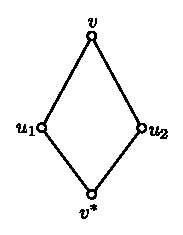
\includegraphics{vol21-figures/fig21-1.eps}}
    \end{figure}
  \end{minipage}

  Then if $j=K$, then $u_1 \equiv u_2$ (trivially).
\end{proof}

If $j=K-1$, then $e^{m_1}_{i_1}e^{m_{k+1}}_{i_{k+1}}=e^m$, say, and 
$$
u_1 \equiv e^{m_1}_{i_1}\cdots
e^{m_{j-1}}_{i_{j-1}}e^{m_{k+2}}_{i_{k+2}}\cdots e^{m_n}_{i_n}\equiv
u_2. 
$$

Finally, if $j <k-1$, put
$$
v^*=e^{m_1}_{i_1}\cdots e^{m_{j-1}}_{i_{j-1}}e^{m_{j+2}}_{i_{j+2}}
\cdots e^{m_{k-1}}_{i_{k-1}} e^{m_{k+2}}_{i_{k+2}} \cdots
e^{m_n}_{i_n}. 
$$

Then $v^*$ is obtained from $u_1$ by the elementary reduction that
deletes $e^{m_k}_{i_k}e^{m_{k+1}}_{i_{k+1}}$ and from $u_2$ by
similarly deleting $e^{m_j}_{i_j} e^{m_{j+1}}_{i_{j+1}}$. 

We now give an intuitive argument to show that if two normal words are
trivially equal, then they are identical. Let $w,w'$ be two words such
that $w = w'$ is a trivial relation. By lemma 1, there exists words
$w=v_0,v_1, \ldots, v_n=w'$ such that either $v_{i+1}$ is obtained
from $v_i$ by elementary reduction or vice versa, for $i=0,1, \ldots
,n$. In the following figure we write $v_{i+1}$ above $v_i$ and
connect it to $v_i$ if $v_{i+1}$ is obtained from $v_i$ by elementary
reduction. 

\begin{figure}[H]
  \centering{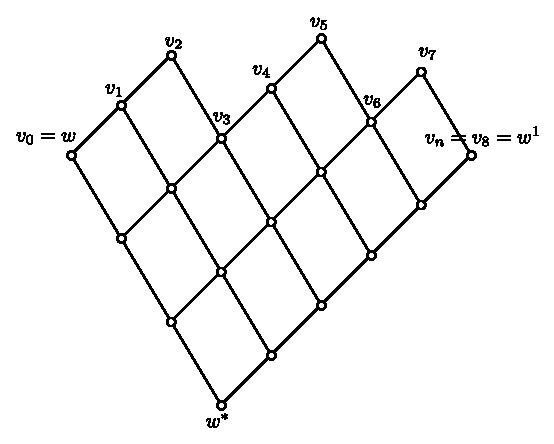
\includegraphics{vol21-figures/fig21-2.eps}}
\end{figure}
a glace at the above figure shows that by several applications of the
diamond lemma, we descend down to a word $w^*$, which is trivially
equal to $w$ and $w'$, or $w$ and $w'$ are identical. Now if $w$ and
$w'$ are normal words which are trivially equal, then they have to be
identical as further descent is not possible. 

A formal proof of the above lemma can be found in M.H.A Newman (1942).
\begin{corollary}
  If $G=gp(E)$, then every element $g \in G$ has a representation
  $g=w(\underbar{e})$ where $w$ is normal. 
\end{corollary}

In particular in a free group, every element is representative by one
and only one normal word. This follows from the fact that in a free
group there are no non-trivial relations. 

\section {}% sec 3

Let $G$ be any group with $G=gp(E; R)$ and $F=gp(E^0, \varphi)$ a free
group such that $|E^0|=|E|$. There is a mapping $\varphi$ of $E^0$
onto $E$ which is one-one. By Von Dyck's theorem $\varphi$ can be
extended to an epimorphism $\varphi^*$ of $F$ onto $G$. 

Let $N=\{ 1 \}^{\varphi *^{-1}}$ be the kernel of $\varphi^*$. Then $N
\Delta F$. Let $f \in F$. Then $f=w(\underbar{e}^0)$. Without loss of
generality we can assume that $w$ is a normal word. We have 
$$
\displaylines{\hfill 
  f^{\varphi^*}=w(\underbar{e})=g \in G \hfill \cr
  \text{where}\hfill e^0=(e^0_1, \ldots, e^0_n)\hspace{1cm}\hfill }
$$
$$
  e^0=(e_1, \ldots, e_n) \text{ and } e_i=e^{0^?}_i.
$$

Now $f \in N$ if and only if $g=1$; i.e., $f \in N$ if only if
$w(\underbar{e})=1$ is a relation in $G$. Fine any relation of $G$ can
be written in the form $w=1$, it follows that $N$ completely
determines the relation in $G$. Hence $N$ is called the
\textit{relation group} of $G$. 

Further
$$
g \cong F/N.
$$
Thus we have the following theorem.

\begin{Theorem}%Thm 3
  Every group is an epimorphis image of a free group and hence in
  isomorphic to a quotient group of a free group. 
\end{Theorem}

If a set of defining relation $R$ of $G$ is given we can say something
more about the structure of $N$. Let $R=\{ f_i \equiv w_i
(\underbar{e})=1 \bigg| i \in I \}$ be a set of defining relation of
$G$. Without loss of generality we can assume that all $w_i
(\underbar{e})$ are normal words. We claim that $N$ is the normal
closure in $F$ of $\{ f'_i\}_{i \in I}$, where
$f'_1=w_i(\underline{e^0})$. That is to say $N$ is the normal subgroup
of $F$ containing $\{ f'_1 \}_{i \in I}$. In other words, if $R'=\{
f'_1 \}_{i \in I}$, then 
$$
N=\bigcap_{R' \subset M \Delta F} M
$$

Since $R' \subset M \Delta F$, we have $N' \subset N$, where $N'$
denotes the normal closure of $R'$. Consider now the quotient
$F/N'$. All the defining relation $w_i=1,i \in I$ of $G$, are
satisfied in $F/N'$ as $R' \subset N'$. Hence any relation $w=1$
satisfied in $G$ is also satisfied in $F/N'$. Let $f \equiv w(e^0)\in
N$. Then $w(e)=1$ is a relation in $G$ and therefore
$w(e^0)N'=N'$. i.e., $w(e^0)\in N'$. Hence $N \subset N'$.  

In virtue of the reversed inclusion which we already have, this proves
that $M=N'$. 

The following theorem gives a method of construction for $N'$.
\begin{Theorem}% Them 4
  Let $G$ be any group, $S \subset G$. Then the normal closure $T$ of
  $S$ in $G$ is the totality of all elements $t$ of the form 
  $$
  t=g^{-1}_1 s^{m_1}_1 g_1 g^{-1}_1 s_2^{m_2}g_2 \cdots g^{-1}_
  \lambda s_ \lambda^m g_ \lambda,
  $$
  where $m_i=\pm1, \lambda$ arbitrary, $g_1,s_i$ are arbitrary
  elements of $G$ and $S$ respectively. 
\end{Theorem}

\begin{proof}
  Let $T$ denote the totality of such elements. Trivially $T$ is
  contained in the normal closure of $S$. To complete the proof of the
  theorem, we have only to show that $T \Delta G$. That $T$ is closed
  under right division is easy to verify, so that $T \leq G$. If $g
  \in G$, then  
  \begin{align*}
    g^{-1}tg &=g^{-1}g^{-1}_1g_1g^{-1}_1 s^{m_2}_2 g_2 \cdots g^{-1}_
    \lambda s_ \lambda ^m g_ \lambda g\\ 
    &= (g_1 g)^{-1}s^{m_1}_1 (g_1 g)(g_1
    g)(g_2g)^{-1}s_2^{m_2}(g_2g)\cdots (g_ \lambda g)^{-1}s^{m} (g_
    \lambda g)\in T 
  \end{align*}
  for arbitrary  $t \in T$. Therefore $T \Delta G$. Hence the theorem.
  Determining to our $N$, we see that $N$ consists of all elements of
  the form 
  $$
  t^{-1}_1 w^{\pm 1}_{i_1}t_1t_2^{-1}w^{\pm 1}_{i_2} t_2 \cdots t_
  \lambda^{-1}w^{\pm 1}_{i_\lambda}, \text{ where } 
  $$
  $t_ \lambda 's$ are arbitrary and $w_{i_k}\in R'$.
\end{proof}

\section{Dual property of free groups} % sec 4.

\begin{Theorem}% Them 5.
  If a group $G$ is epimorphically mapped on a free group $F$, then
  $G$ contains a free subgroup isomorphic to $F$, and in fact mapped
  isomorphically onto $F$ by the restriction to it of the epimorphism
  of $G$. 
\end{Theorem}

\begin{proof}
  Let $\varphi$ be an epirophism of $G$ onto $F$. Let
  $F=gp(E,\varphi)$. Then $e^{\varphi^{-1}}$ is a non-empty every $e
  \in E$. Choose and $e_1$ from $e^{\varphi^{-1}}$. Denote by $E_1$
  the set of all such $e_1's$. Let $F_1=gp(E_1)$. We claim that the
  restriction $\varphi_1$ of $\varphi$ to $F_1$ onto $F$. That the
  mapping $\varphi_1$ is an epimorphism is obvious, by our choice of
  $e_1's$. Now if $g \in F$, let $w(\underbar{e})$ ne a normal word
  representing $g$. Then
  $g^{\varphi_1}=(w(\underbar{e}))^{\varphi_1}=(w(\underbar{e}))^{\varphi}=(w(\underbar{e}^\varphi
  _1))=w(\underbar{e})=1$ if and only if $w$ is the empty word, as $F$
  is a free group. Hence the kernel of $\varphi _1$ consists of the
  netral elements along and therefore $\varphi_1$ is an
  isomorphism. Since any group isomorphic to a free group is also
  free, our theorem follows. 
\end{proof}

\begin{Theorem}%THEM 6.
  Free groups generated by sets of the same cardinality are isomorphic.
\end{Theorem}

\begin{proof}
  Let $E$ and $E^0$ be two sets such that $|E|=|E^0|$, $F=gp(E,\phi)$
  and $F^0=gp(E^0, \phi)$. Let $\psi$ be a one-one mapping of $E^0$
  onto $E$. Extend it to an epimorphism of $F^0$ onto $F$. We shall
  also denote this extended mapping by $\psi$. 
\end{proof}

Now $(w(c^0))^\psi=w(e)=1$ if and only if $w$ is an empty word. This
follows because we can without loss of generality take $w$ to be a
normal word. hence $w(e^0)=1$. Therefore $\psi$ is an isomorphism of
$F^0$ onto $F$. 

This shows that the structure of a free group depends only on the
cardinality of its set of generator. We shall $|E|$ the rank of the
free group $gp(E, \phi)$. A free of rank zero is the trivial group $\{
1 \}$. Free groups of rank $1$ are finite cyclic groups. 

It is natural to ask if free groups of defferent ranks are in fact
defferent. The following theorem answer this question. 
\begin{Theorem} %Them 7
  Free groups of different ranks are not isomorphic.
\end{Theorem}

To prove this theorem we need the following lemma, the proof of which
we shall give later. 
\begin{lemma}
  To every cardinal number $n$ there is group $G_n$ that can be
  generated by a set of cardinal $n$ elements, but by no set of
  strictly smaller cardinal. 
\end{lemma}

\begin{proof of the theorem}
  Let 
  \begin{align*} 
    F_n &= gp(E_n, \phi), |E_n| =n,\\ 
    F_m &=gp(E_m, \phi), |E_m| =m 
  \end{align*}
  where $n$ and $m$ may be infinite cardinals. Choose $G_n$ of the
  above lemma. Then there is a epimorphism $\psi$ of $F_n$ onto
  $G_n$. Assume that there is an isomorphism of $F_m$ onto
  $G_n$. $\varphi$ of $F_m$ onto $F_n$. Then $\varphi \psi$ is an
  epimorphism of $F_m$ onto $G_n$.  Therefore $E_m^{\varphi \psi}$
  generates the group $G_n$. Hence we have $m=|E_m|\geq |E_m^{\varphi
    \psi}|\geq n$ using the isomorphism $\varphi^{-1}$, we similarly
  if $m \neq n$. Hence the theorem.  
\end{proof of the theorem}
 
\begin{proof of lemma}
  For every cardinal $n$, we shall construct a $G_n$ with the desire
  property. Let $M$ be any set with $|M|=m$. Consider the set $G$ of
  all finite subsets of $M$. We turn $G$ into a group by defining the
  binary operation as the symmetric difference. That is to say, for
  every $S,T \varepsilon G$. 
  $$
  ST=(S-T)\bigcup (T-S)
  $$
  We take the empty set $\phi$ as the unit element and each $S$ as its
  own inverse. For we have 
  $$
  S \phi=\phi S=S \text{ and }SS=\phi, \text{ for every } S \varepsilon G.
  $$

  The verification of the associativity of this multiplication is easy
  and therefore we omit it. Hence the multiplication defined in $G$,
  make $G$ a group. We  claim that this group $G$ is generated by the
  set of one-element subset of $M$, $E= \bigg \{ \{ x\} \bigg | x \in
  M \bigg \}$. For if $S=\bigg \{ a_1,a_2, \ldots, a_k \bigg \}$, it
  is easily seen that $S=\{ a_1\} \{ a_2\} \cdots \{ a_k \}$. Further
  for every $S$, $T \varepsilon G$, we have $ST=TS$. Therefore $G$ sin
  commutative. We shall show that no set of cardinal $<m$ generates
  $G$. Let $E^0$ be a set of generators of $G$ with $E^0=n$, say. Then
  every elements $x \varepsilon G$ can be written as 
  $$
  x=s^{m_1}_1 S^{m_2}_2 \cdots S^{m_k}_k \text{ with } m_i=\pm1, S_i
  \varepsilon E^0, i=1,\ldots, k. 
  $$

  But in $G$, we have $S=S^{-1}$, for every $S \varepsilon
  G$. Therefore every $x \varepsilon G$, can be written as 
  $$
  x=S_1S_2 \cdots S_k \text{ with district generators } S_i \varepsilon E^0.
  $$
  
  Further, since $G$ is commutative it follows that every finite
  subset of $E^0$ determines only one element of $G$. Thus to every
  element $x \varepsilon G$, we can associated a finite subset of
  $E^0$. This shows that $G|\leq$ cardinal of the set of all finite
  subsets of $E^0$. But we know that if $X$ is any set and $F$ the set
  of all finite sebset of $X$. Then 

\noindent $\begin{aligned}
    & |F|= 2^X \text{ if }|X|< \mathcal{N}_0\\
    \text{ and } \hspace{3cm} &|F|= X \text{ if }|X|\geq \mathcal{N}_0
  \end{aligned}
$

  Thus if $m$ is finite, we have, from the above inequality, that $2^m
  \geq 2^n$, and therefore $m \leq n$. If $m$ is infinite and $n$ is
  finite, we have $m \leq 2^n$, which is impossible. Hence if $m$ is
  infinite, $n$ must also be infinite, and again conclude that $m \leq
  n$. Hence the group $G$ cannot be generated by a set of cardinals
  strictly smaller than $m$. This establishes the lemma. 
\end{proof of lemma}

\chapter{Identical Relations and Varieties of Groups.} % chapter 5.

\section{} % sec 1.

In the preceding chapter we have seen that an arbitrary mapping from a
set generators of a free group into any other group can be extended to
a homomorphism. In fact this property completely characterises the
free groups. In order to generalise this notion of being ``free", we
introduce certain classes of groups called \textit{vareties} of groups  

While proving that the free groups of different ranks are not
isomorphic we have come across an example of a group $G$ in which the
equation $x^2 =1$ holds for all $x$ in $G$. Such equations are called
\textit{identical relations} or \textit{laws}. 
\begin{definition}
  A law or identical relation is a relation of the form
  $$
  u (\underbar{X}) = v(\underbar{X})
  $$
  where $u$ and $v$ are words in $\underbar{X} = (X_1, \ldots, 
  X_n)$. We say that the law $u (\underbar{X}) = v(\underbar{X})$
  holds in a group $G$ if the equation $u (\mathfrak{f} =
  v(\mathfrak{f}))$ holds when we substitute arbitrary elements $g_1,
  \ldots,  g_n$ of $G$ for the ``variables" $X_1, \ldots,  X_n$. For
  instance if $u(\underbar{X}) = X_1 X_2$ and $v (\underbar{X})= X_2
  X_1$, then in an abelian group the law $u (\underbar{X}) =
  v(\underbar{X})$ holds.  
  
  The following fundamental relations can be easily verified 
  \begin{enumerate}[\rm (1)]
  \item If $u \equiv v$, then $u = v$ is a law.
  \item If $u = v$, is a law then so is $v= u$.
  \item If $u = v$ and $v = w$ are laws, then so is $u = w$.
  \item If $u = v$ and $u' = v'$ are laws, then $uu' = vv'$ is a law.
  \item $XX^{-1} = 1$ and $X^{-1}X =1$ are laws.
  \item If $u (\underbar{X}) \equiv u (X_1, \ldots,  X_n) = v(X_1,
    \ldots,  X_n) \equiv v(\underbar{X}) $ is a law and $Y_1
    (\underbar{Z})$, $\ldots Y_n (\underbar{Z})$ are words in variables
    $Z_1, \ldots,  Z_p$ then $u (Y_1(\underbar{Z}) \ldots Y_n
    (\underbar{Z})) = v (Y_1(\underbar{Z}), \ldots,  Y_n
    (\underbar{Z}) )$ is a law. 
  \end{enumerate}
\end{definition}

The rule $(7)$ is a called the \textit{substitution rule}.

[If we assume $XX^{-1} =1$ and $(7)$ we can derive the law $X^{-1}X =
  1$. For put $Y = X^{-1}$. Then $YY^{-1} =1$ is a law. i.e. $X^{-1}
  (X^{-1})^{-1}= X^{-1} X=1$ is a law.] 

These rules can be used can be used to derive from given laws that are
valid in a group further laws that ``follow" from the given laws. 

\begin{example}
  If $X^2 = 1$ is a law in a group, then so is
  $$
  XY = YX
  $$
\end{example}

\begin{proof}
  The law $XY = YX$ is equivalent to $X^{-1} Y^{-1} XY = 1$. Now 
  \begin{align*}
    X^{-1} Y^{-1} XY & = X^{-1}Y^{-1} XX^{-1} Y^{-1}XX^{-1}X^{-1} XYXY\\
    & = (X^{-1} Y^{-1}X)^2 (X^{-1})^2 (XY)^2
  \end{align*}
  Applying $(5)$ and $(7)$ we have $X^{-1}Y^{-1}XY = 1$, i.e. $XY =
  YX$ is a law.  
\end{proof}

It is easily seen (as for relations) that every law $u(\underbar{X}) =
v(\underbar{X})$ is equivalent to a law $w (\underbar{X}) = 1$; and it
is often convenient to write all laws in this from. 

\section{Varieties} % sec 2.

Throughout this chapter we shall assume that the set of variables 
$\bigg\{ X_1, X_2$, $\ldots \bigg\}$ is countable. This is just for
convenience and not a real restriction. 

Let $L$ be a set of laws invariables $\bigg\{ X_1, X_2, \ldots
\bigg\}$. The class of all groups satisfying the laws of $L$ is called
\textit{variety}. We call this the variety \textit{defined} by $L$ and
denote it by $V_{=L}$ as it clearly depends on $L$. For example if $L$
consists of the single law $X^{-1}_1 X^{-1}_2  X_1 X_2 =1$, then
$V_{=L}$ is the class of all abelian groups. 

A variety may be defined by different sets of laws. For instance if $L
= \bigg\{ X^2_1 = 1\bigg\}, L' = \bigg\{ X^2_1 = 1, X^{-1}_1X^{-1}_2
X_1 X_2 = 1\bigg\}$, then $V_{=L}= V_{=L'}$. 

It is easily seen that if $L \subseteq L'$, then $V_{=L'} \subseteq
V_{=L}$. We say that a variety $\underset{=}V$ is \textit{finitely
  based} if there exists a finite set of laws defining
$\underset{=}V$.  

In this context there are still some undecided questions. 

\begin{problem}
  Are all varieties of groups finitely based?
\end{problem}
 
Let $\underset{=}C$ be a class of groups, and consider the ``least
variety" to which all groups of  $\underset{=}C$ belong: thus is the
variety defined by all those laws that are (simultaneously ) valid in
all groups in $\underset{=}C$. We can take, as the simplest case
$\underset{=}C$ to consist of just a single group $G$. 

\begin{problem}
  If $\underset{=}V$ is the least variety to which the finite group
  $G$ belongs, is $\underset{=}V$ necessarily finitely based?   
\end{problem}
 
Even this problem is not solved in general; only if $G$ is further
assumed to be nllpotent is the answer known to be positive
[R.C. Lyndon $1952$]; of. also $p.163$. 

Let $V_{= L}$ be a variety, without loss of generality we can assume
that all laws in $L$ are of the form $w=1$, where $w$ is a normal word
in the variables $X_1,X_2,\ldots $. Let $E$ be any set with
$|E|=n$. Let $RF$ be the set of all relations of the form
$w(e_1,\ldots,e_m)=1$ with $e_i$ arbitrary elements of $E$ and $w(X_1,
\ldots, X_m)=1$ a law in $L$ and $m \leq n$. Consider the group $F_L =
gp(E;R)$. Now, if $G$ is a group in the variety $V_{=L}$, then any
mapping $\varphi$ of $E$ into $G$ is extendable to a homomorphism
$\varepsilon^*$ of $F_L$ into $G$. For if $w(e_1,\ldots,e_n)=1$ is a
relation in $R$, then $w(X_1,\ldots,X_n)=1$ is a law in $L$; and
therefore, since $G \varepsilon V_{=L}, w(e^\varphi_1,
\ldots,e^\varepsilon_n)=1$ is a relation in $G$. Thus the set $R$ of
defining relations in $F_L$ go over to relations in $G$ upon applying
$\varphi$ 

Therefore, by von Dyck's theroem the mapping $\varphi$ is extendable
to a homomorphism $\varphi^*$ of $F_L$ into $G$. Thus in a way, this
is a generalisation of free groups, We call $F_L$ a \textit{free group
  of} $V_{=L}$ (reduced free or relatively free) of rank $n$. It is
easy to see that $F_L$ itself is a member of $V_{=L}$ and it depends
upon $n$. In particular if $L$ is the empty set we get the free group
in the ordinary sense (in this context called \textit{absolutely free
  groups)}. 

\section{Burnside conjectures}%Sec 3.

Let $L$ be the set consisting of the single law $X^n=1$. We denote the
corresponding $V_{=L}$ by $B_{=n}$. Group of $B_{=n}$ are called
groups of \textit{exponent} $n$. We call $B_n$ the \textit{Burside
  variety} after $W$.  
Burnside (1852-1927). There is a problem connected with this known as
the Burnside conjectures (Burnside $W.1902$). We first state the
original conjecture, now known as the Full Barnside Conjecture; and
afterwards a weaker from, the so-called Restricted Burnside
Conjecture. \textit{Full Burnside Conjecture}. Every finitely
generated group in $B_{=n}$, that is of finite exponent $n$, is
finite. Let $B_{d, n}$. denote a $d$ generator free group of
$B_{=n}$. The Full Burnside Conjecture is equivalent to saying that $|
B_{d, n}| < \mathscr{N}_\circ$, for every positive integer $d$ for
every group with $d$ generators and exponent $n$ is an epimorphic
image of $B_{d, n}$. 

The following problem is weaker than the above conjecture.

\noindent
 {\bf Restricted Burnside Conjecture.}

There is a bound $\beta(d, n)$ such that every finite $d$ generator
group of exponent $n$ has order $\leq \beta(d, n)$. This conjecture is
an easy consequence of the full Burnside conjecture. For if the full
conjecture is true, then $B_{d, n}$ is finite and we can take
$\beta(d, n) = |B_{d, n}|$. The present state of knowledge of the
Burnside conjecture is for from complete. The following are the
results so far obtained in this direction. In the following $d$
denotes the number of generators, $n$ the exponent. We abbreviate the
Restricted Burnside  

Conjecture and the full Burnside conjecture $RBC$ and $FBC$
respectively. 

\noindent 
\begin{tabular}{cccccp{4.5cm}}
\hline
\hline
d & n & RBC & FBC & &REMARKS \\
\hline
all & $2$ & & true & &Trivial. In fact $|B_{d,2}|=2^d$.\\
all & $3$ & & true & &Burnside (1902). The order of $B_{d,2}$ was given
by Levi and van der Waerden (1933).
 $|B_{d,3}|=3^{\binom{d}{1}+\binom{d}{2}+\binom{d}{3}}$. \\
all & 4 & & true & &Sanov(1940). The irder of $B_{d,4}$ is not known.\\
$2$ & $5$ & true & unsolved & &Kostrikin (1955). \\
all & $5$ & true & unsolved & &G.Higman (1956). \\
all & $6$ & true & &  &P. Hall and G. Higman (1956). \\
all & $6$ &  & true &   &M. Hall, Jr. (1959).\\
all & $12$ & true & unsolved & &P. Hall and G. Higman (1956). \\
all & all prime & p true & - & &Kostrikin(1959).\\
all & \multicolumn{1}{p{1.3cm}}{$pq$  ($p, q$ different primes)} &
true & unsolved  &   {\Bpara{-8}{-15}{180}{30}}&
      \raisebox{-.2cm}{\multirow{3}{4.5cm}{follows form a  conination of Kostrikind (1959),
      Hall and Higman(1956)}}\\
all &  \multicolumn{1}{p{1.3cm}}{4p (p, a prime)}&  true & unsolved&&   \\
$2$ & $\geq $ & $72$ &  not true & &Novikov(1959).\\
\hline
\end{tabular}

\section{A consequences of the result of Novikov (1959) and Kostrikin
  (1959).}%4 

using the result of Novikov and Kostrikin, we shall derive an
interesting consequences. As the Burnside conjecture is not true for
$d=2, n \geq 73$, it follows that $B_{2,73}$, the $2$ generator free
group of $B_{=73}$, is infinite. But $73$ is a prime, and therefore by
Kostrikin's result, there exists a maximal finite $2$ generator group
of exponent $73$. Let us denote this group $B^*_{2,73}$. We know that
$B^*_{2,73}$ is an ipimorphic image of $B_{2,73}$ and therefore is
isomorphic to a quotient group of $B_{2,73}$. Thus $B^*_{2,73} \cong
B_{2,73}/N, N \Delta B_{2,73}$. Therefore $N$ is an infinite normal
subgroup of finite index in $B_{2,73}$. We now state the following
theorem without proof. 

\begin{theorem}
  (0, Schreier (1972); see Kurosh (1956) pp.36-37). A subgroup
  of finite index of a finitely generated group is finitely
  generated. 
\end{theorem}

By this theorem $N$ is finitely generated. Now, it is known that a
finitely generated group contains a maximal normal
subgroup. (B.H. Neumann $1937^b$). Let $M$ be a maximal normal
subgroup in $N$. 
Then it is easily seen that $N/M$ is simple; that is to say, $N/M$
does not contain any proper non-trivial normal subgroup. We assert
that the group $N/M$ is infinite. To prove this we quote another
theorem with out proof. 

\begin{theorem}[R. Baer $1953$]
  If a finitely generated group contains a proper subgroup of finite
  index it also contains a characteristic (for definition see section
  $6$ of this chapter) proper subgroup of finite index. 
\end{theorem}

If $N/M$ is finite, by the above theorem, there exists a
characteristic proper subgroup $K$ of finite index in $N$. It follows
that $K$ is a normal subgroup of $B_{2,73/K}$ and is of finite index
in $B_{2,73}$. Therefore $B_{2,73/K}$ is a finite group of exponent
$73$, whose order exceeds that of $B^*_{2,73}$. This is
impossible. Therefore $N/M$ is infinite. Thus we arrive at in infinite
group $N/M$ which is simple, finitely generated and of exponent 73. 

\section{}% 5

We return to the considerations of section $2$. Let $V_{=L}$ be a
variety determined by a set of laws $L$. Without loss of generality we
can assume that every law of $L$ is of the form $w(X_1,\ldots,X_n)=1$
where $w(X_1,\ldots,X_n)$ is a normal word in the variables $X_1,
X_2,\ldots$. We denote by $F_n$ the free group generated by the
variables $X_1, X_2, \ldots,X_n$ and by $F$ the free group generated
by all the variables $X_1, X_2,\ldots$. That is to say, 
$$
F_n =gp\left(\bigg \{X_1,\ldots, X_n \bigg \}, \phi\right),~F_\omega = gp
\left(\bigg\{X_1, X_2,\ldots \bigg\}, \phi\right) 
$$

By $F$ we shall mean either $F_n$ or $F_\omega$. With every $V_{=L}$
we associate a subgroup $W$ of $F$ in the following way. Define 
\begin{equation*}
  \left\{
  W=
  w(X_1,\ldots,X_m) \Bigg|
  \begin{aligned}
    & w(X_1,\ldots,X_m)=1 \\
    & w(X_1,\ldots,X_m) \varepsilon^F
  \end{aligned}
  \text{ valid in all group } of ~V=L
  \right\}
\end{equation*}
That $W$ is a group is easy to verify.

Now let $F_L$ be a free group of $V_{=L}$ with $E$ as the set of
generators and of the same rank as $F$. Consider some one-one mapping
$\varphi$ of $X$ onto $E$, where $X$ denotes the set of generators of
$F$. We can extend $\varphi$ to an epimorphism $\varphi^*$ of $F$ onto
$F_L$. The kernel of $\varphi^*$, by the definition of $F_L$, is
precisely the group $W$ we have defined above. Therefore $W$ is a
normal subgroup of $F$ and $F_L$ is isomorphic to $F/W$. The
substitution rule which we have for laws in a group gives some more
information about $W$. If $w(x_1, X_2, \ldots, X_m)\varepsilon W$, and
$Y_1(\underbar{X}),\ldots,Y_m(\underbar{X}) \varepsilon F$, then also
$w(Y_1(\underbar{X}),\ldots,Y_m(\underbar{X})) \varepsilon W$.  
 
We make the following definition.

\begin{definition}
  Let $E$ be any set, $S \subseteq E$ and $\eta$ a mapping of $E \to
  E$. We say that the subset $S$ admits the mapping $\eta$ if $S^\eta
  \subseteq S$. 
\end{definition}
 
\setcounter{Theorem}{0}
\begin{Theorem}%Thm 1
  The subgroup $W \leq F$ admits all endomorphisms of $F$.
\end{Theorem} 
 
\begin{proof}
  Let $\eta$ be any endomorphism of $F$ and $X^\eta_i =
  Y_i(\underbar{X})$. If $w(X_1,\ldots, X_m)$ is in $W$, then 
  \begin{align*}
    \bigg ( w(X_1,X_2,\ldots, X_m) \bigg) ^\eta & = w (X^\eta_1,\ldots
   , X^\eta_m)\\
    & = w(Y_1(X),\ldots, Y_m(X)) \varepsilon W.
  \end{align*}
  Therefore $W^\eta \subseteq W$. This proved the theorem.
 \end{proof} 
 
Let $G$ be any group. For every $t \varepsilon G$, we define the
mapping $\varepsilon_t$ of $G$ onto itself such that 
$$
x^{\varepsilon_t} = t^{-1} xt \text{ for all } x \varepsilon G.
$$
now $(xy)^{\varphi_t}=t^{-1} x y t = (t^{-1}x t) (t^{-1} y
t)=(x)^{\varphi_t} y^{\varphi_t}$ for all $x$ and $y$ in
$G$. Therefore $\varphi_t$ is an endomorphism of $G$. But 
$$
x^{\varphi_t \varphi_{t-1}} = (t^{-1}x t)^{\varphi_t} = t(t^{-1} x
t)t^{-1} = x = x^{\varphi_t -1 \varphi_t}. 
$$
Thus $\varphi_t \varphi_t -1 = \ell = \varphi_t -1 \varphi_t$; in
other every $\varphi_t$ has a two sided inverse. Thus $\varphi_t$ is
an automorphism of $G$. We call $\varphi_t$ an \textit{inner
  automorphism} of $G$. An automorphism which is not an inner
automorphism is called an \textit {outer automorphism}. 
  
 Let us denote by $A_I$ the set of all inner automorphisms of $G$. It
 is easy to see that $A_I$ is a group. There is a natural mapping
 $\varphi$ of $G$ onto $A_I$ defined by $s^\varphi = \varphi_s$ for
 all $s$ in $G$. This mapping $\varphi$ is easily seen to be an
 epimorphism. Then kernel $Z$ of $\varphi$ consists precisely of those
 elements of $G$ which commute with every element of $G$. [For proofs
   see Kurosh ($1955$), Ch. $4$, $\S 12$]. We call $Z$ the center of
 $G$. By the definition of inner automorphisms it follows that $N
 \Delta G$ if and only if $N$ admits all inner automorphisms of $G$. 
 
A subgroup $H \leq G$ is \textit{characteristic} in $G$ if it admits
all automorphisms of $G$. Similarly a subgroup $H$ ~$G$ is
\textit{fully invariant} in $G$ if it admits all endomorphisms of
$G$. By the definition of full invariance it follows that the subgroup
$W$ in Theorem $1$ is fully invariant in $F$. Every fully invariant
subgroup of $G$ is trivially characteristic in $G$ and every
characteristic subgroup of $G$ is normal in $G$. We remark that the
centre $z$ of a group $G$ is a characteristic subgroup. For if a $a
\varepsilon Z$, then $ax = xa$ for every $x$ in $G$. Therefore 
$$
a^\top x^\top = (ax)^\top = (xn)^\top = x^\top a^\top
$$
for every automorphism $\top$ of $G$. Now since $x^\top$ runs through
all the elements of $G$ it follows that $a^\top$ is in $Z$ and
therefore $Z$ is a characteristic subgroup of $G$. In general the
centre of a group is not a fully invariant subgroup. [See Kurosh
(1955), ch. 4 ~15]. 
 
One can easily verify that the intersection of an arbitrary family of
characteristic (fully invariant) subgroups of a group is a
characteristic (fully invariant) subgroup. Thus we can talk of
characteristic (fully invariant subgroup generated by a set of
elements and also of the lattice of characteristic (fully invariant)
subgroups of a group. 
 
In general a characteristic subgroup is not a fully invariant
subgroup. ;[See Neumann and Neumann (1951)]. The following is an
unsolved problem in this direction. 
 
\begin{unsolved problem}
  Is there a charactercristic subgroup of a free group $F$ of infinite
  rank which is NOT fully invariant in $F$? 
\end{unsolved problem} 
 
\begin{Theorem}
  The relation "characteristic" and "fully invariant" are transitive;
  that is to say, if $K \leq H \leq G$ with $K$ characteristic (fully
  invariant) in $H$ and $H$ characteristic (fully invariant) in $G$
  then $K$ is characteristic (fully invariant) in $G$. 
\end{Theorem} 
 
\begin{proof}
  Let $\alpha$ be an automorphism of $G$;~ $\alpha'$ the restriction
  of to $H$. Then, because $H$ is characteristic in $G, H^\alpha \leq
  H$. Applying the automorphism $\alpha^{-1}$ to $H$, we have
  $H^{\alpha-1} \leq H$. Therefore $H=(H^{\alpha-1})^\alpha \leq
  H^\alpha$. Hence we have $H^\alpha = H$. i.e. $H \quad =H$.Therfore
  $\alpha'$ is an automorphism of $H$. Now since $K$ is characteristic
  in $H$, we have $K^\alpha = K^\alpha \leq K$. hence $K$ is
  characteristic in $G$. 
\end{proof} 
 
The proof in the case of full invariance is similar and actually even
easier and we omit it. 
 
The transitivity is not true for the relation "normal". In other words
if $K \Delta H \Delta g$, in general it is not true that $K \Delta
G$. For example take for $G$ the symmetric group $S_4$ of permutations
on four letters or the alernating group $A_4$. Let 
\begin{align*}
  H & = V_4 = \bigg\{ 1, (12)(34), (13)(24), (14)(23)\bigg \} ~~\text{ and } \\
  K & = \bigg \{1, (12) (34)\bigg \}.
\end{align*} 
 We know that $H \Delta G$, and $K \Delta H$. Now $(123) \varepsilon
 A_4$. $(123)^{-1} = (132)$ and $(123)^{-1}K(123) = \bigg \{1, (14)
 (23)\bigg \} \neq K$. 
 
We say that $H \leq G$ is \textit{accessible} (or \textit{subnormal})
in $G$ (notation $H \Delta \Delta G)$ if there exists subgroups $H_0 =
H, H_1,\ldots, H_n = G$, such that $H_0 \Delta H_1 \Delta H_2 \cdots
\Delta H_n $. 
 
The accessible subgroups of finite group were introduced by
H. Wielandt ($1939$) and further studied by H. Wielandt and recently
by B. Huppert. It is easy to verify that the intersection of two and
hence the intersection of a finite number of accossible subgroups is
an accessible subgroup. The intersection of an infinite number of
accessible subgroups need not be an accessible subgroup. 
 
If a group $G$ has a composition series [Kurosh (1955), $CH. 5, \S
  16$] then the join of any two accessible groups is again an
accessible group (Wielandt (1939)). The following is an unsolved
problem. 
 
\begin{unsolved problem}
  Is the join of two accessible subgroup of an infinite group (without
  composition series) accessible? 
\end{unsolved problem} 
 
\section{Verbal Subgroups}%Sec 6
 
Let $L$ be any set of words \footnote{This is a slight change of
  notation - earlier $L$ stood for a set of laws $=1$, now only for
  the set of their left-hand sides.} in the variables $X_1, X_2,\ldots
$ and $G$ a group. Consider the set, 
 $$
 S= \Bigg \{w(g_1,\ldots,g_n) \bigg | w(x_1,\ldots,x_n)\varepsilon L, 
 g_i \varepsilon G i=1,2,\ldots n \Bigg\} 
 $$
 This is not in general a subgroup of $G$. We call $H=gp(S) \leq G$,
 the word \textit{subgroup} or a \textit{verbal subgroup} defined by
 $L$. 
 
\begin{Theorem}%Thm 3
  Every verbal subgroup $H$ of a group $G$ is fully invariant.
\end{Theorem}
 
\begin{proof}
  Let $\eta$ be an endomorphism of $G$ and the verbal subgroup $H$ be
  defined by $L$. It is enough to prove that $S^\eta \subseteq S$, for
  every endomorphism $\eta $ of $G$, where $S$ is the set of
  generators of $H$ as defined above. Now if $w(g_1,\ldots 
 ,  g_n) \varepsilon S, w(X_1,\ldots,X_n)\varepsilon L_\eta
  $, then $\bigg\{w(g_1,\ldots,g_n)\bigg \}^\eta = w(g^\eta
  _1,\ldots$, $g^\eta_n) \varepsilon S$. Therfore $S^\eta \subseteq S$;
  this is true of every endomorphism of $G$. Hence $H$ is fully
  invariant in $G$. The converse of this theorem is not true in
  general; but happens to be in the case of free group. 
\end{proof}  
 
\begin{Theorem}%Thm 4
  Every fully invariant subgroup of a free group is verbal.
\end{Theorem} 
 
\begin{proof}
  Let $W$ Be a fully invariant subgroup of a free group $F$. Let $L$
  be the set of all normal words that occur in $W$. If
  $Y_1(\underbar{X}),  \ldots,Y_n (\underbar{X}) \varepsilon F$, where
  $\underbar{X}=(x_1,\ldots,X_n)$ and $X_i \varepsilon X$, and where
  $X$ denotes the set of variables as well as the set of generators of
  $F$, then the mapping defined by 
  $$
  X^\eta_i = Y_i (\underbar{X}), ~ i = 1,\ldots,n,
  $$
  can be extended to an endomorphism of $F$ which also we denote by
  $\eta$. 
  Now if $w(X_1,\ldots,X_n) \varepsilon L$, then
  $w(X_1,\ldots,X_n)^\eta =
  w(Y_1(\underbar{X}),\ldots,Y_n(\underbar{X}))\varepsilon W$ as $W$
  is fully invarient in $F$. Therfore  
  $$
  S= \Bigg \{w(Y_1(Y_1(\underbar{X}),\ldots,Y_n (\underbar{X})) \bigg |
  w(X_1,\ldots,X_n)\varepsilon L,   
  Y_i (\underbar{X}) \varepsilon F,  i=1,2,\ldots n \Bigg\}
  $$
  is contained in $W$. But clearly also $W \subseteq S$. Thus $S=W$, and
  also $gp(S)=W$. Hence the theorem. 
\end{proof}

It follows that the intersection of any arbitrary family of verbal
subgroup of a free group is a verbal subgroup. In general in an
arbitrary group this is not true [B.M. Neumann $(1937^a)$]. It is easy
to verify that the join of two verbal subgroup of a group is a verbal
subgroup. 

\section{}%7.

We shall now give an important example of a verbal subgroup. Let $G$ be
any group. Let $L$ consist of the single word $X^{-1}_1 X^{-1}_2 X_1
X_2 = [X_1, X_2]$. The verbal subgroup $G'$ of $G$ defined by $L$ is
called the \textit{commutator subgroup} or \textit{derived subgroup}
of $G$. 
  
Evidently the commutator subgroup of an abelian group is the trivial
group. For any group it is easily seen that the quitient group $G/G'$
is ableian [Kurosh (1955)]. 
  
\begin{Theorem}%Thm 5
  Let $W$ be a verbal subgroup, defined by a set $L$ of words, of the
  free group $F$. Then the quotient group $F/W$ is the free group of
  the varisety $V_{=L}$ defined by the laws $w(\underbar{X})1$, for
  all $w(\underbar{X}) \varepsilon L$ and it has the same rank as
  $F$. 
\end{Theorem}  
  
\begin{proof}
  Now $F_L$, the corresponding free group of the variety $V_{=L}$, is
  isomorphic to $F/W^*$, where $W^*$ consists of all $w(X_1, \ldots,
  X_n)$ such that $W^*$ is fully invariant in $F$. If $w(X_1,\ldots,
  X_n)$ is in $L$, then $w(Y_1(\underbar{X}), \ldots,(\underbar{X}))
  \varepsilon W^*$ for arbitrary $Y_i (\underbar{X}) \varepsilon
  F$. Therefore $W \leq W^*$. Now $F/W \varepsilon V_{=L}$. Therefore,
  if $w(X_1, \ldots, X_n) \varepsilon W^*$ then the law $w(X_1,\ldots
 ,  X_n)=1$ holds in $F/W$. In other words $w(X_1,\ldots,X_n)
  \varepsilon W$. Therefore $W^* \leq W$; we get $W = W^*$. Hence the
  theorem. 
\end{proof}  
  
\begin{Theorem}%Thm 6
  Every verbal subgroup $W$ of a free group $F$ is the fully invariant
  closure of the set $L$ (i.e. the fully invariant subgroup generated
  by $L$) of words consisting of either one or no word of the from
  $X^k_1$ and apart from that "commutator words" i.e. words contained
  in the drived group $F'$. 
\end{Theorem}  
  
\begin{proof}
  We have already remarked that the quotient group $F/F'$ is
  abelian. Therfore every $w \varepsilon W$ can be written as
  $w=X^{k_1}_1 \cdot X^{k_n}_n w'$ with $w' \varepsilon F'$. Let
  $\eta$ be the endomorphism of $F$ defined by $X^\eta_1 = X_1,
  X^\eta_i = 1$ for $i \neq 1$. Since $W$ is fully invariant in $F$ it
  follows that $w^\eta = X^{k_1}_1 w'^{\eta}=X^{k_1}_1$. Similarly
  $\eta_i$ defined by $X^{\eta_i}_i = X_1$ and $X^{\eta_i}_j = 1$ for
  $j \neq i$, generates an endomorphism of $F$ and therefore
  $w^{\eta_i}=w'^{\eta_i}= X^{k_i}_1$, since $w'^{\eta_i}=1$. Let
  $gp(X^k_1) = gp(X_1) \cap W$. Then $k/k_i$ for $i=1,2,\ldots n$. If
  $\Pi_i$ is the endomorphism defined by $X^{\Pi_i}_1 = X_i,
  X^{\Pi_i}_j = 1$ for $i \neq j$, then $(X^k)^{\Pi_i} = X^k_i \varphi
  W$. Let $L$ be the set consisting of $X^k_1$ and all the $w's$ that
  occur when each $w \varepsilon W$ is written as $w = X^{k_1}_1
  \cdots X^{k_n}_n w'$. It is easily seen that any invariant subgroup
  of $F$ that contains $L$ also contains $W$. But $W$ itself is fully
  invariant in $F$. Hence $W$ is the fullyinvariant closure of
  $L$. When $k=0$, $L$ is a subset of $W'$. 
\end{proof}  
  
\begin{corollary}[B.M. Neumann, $1937^1$]. 
  If $k \neq 1$, then the reduced free groups of the variety are
  non-isomorphic for different ranks. [If $k=1$, the free groups of
    the variety are all the trivial groups.] 
\end{corollary}  

\chapter{Group-theoretical Constructions}%Chap VI

\section{The Cartesian product and the direct product of a family of
  groups.}%Sec 1 

Let $\bigg \{G_i\bigg\}_{i \varepsilon I}$ be a family of group
indexed by a non-empty set $I$. Let $T$ denote the set of all
functions on $I$ with values in $G_i$. Consider the set $P$ defined by  
$$
P = \Bigg \{ f \varepsilon T \bigg | f(i) \varepsilon G_i \text{ for
  all } i \varepsilon I \Bigg \}. 
$$
We turn $P$ into a group by introducing the following multiplication:
If $f, g \varepsilon P$. Then 
$$
fg = h, \text{ where } h(i) = f(i) g(i), \text{ for all } i \varepsilon I.
$$
It is easy to see that $h \varepsilon P$. We take the function $e
\varepsilon P$, defined by  
$$
e(i) = 1_i \text{ for every } i \varepsilon I
$$
(where $1_i$ is the unit element of $G_i$) as the unit element. For, 
$$
ef = fe = f, \text{ for all } f \varepsilon P.
$$
For every $f \varepsilon P$, we take the function $f^{-1}$ defined by 
$$
f^{-1}(i) = (f(i))^{-1}, \text{ for every } i \varepsilon I,
$$
as the inverse of $f$. It is easy to verify that $f^{-1} \varepsilon
P$ and $ff^{-1} = f^{-1} f = e$, for every $f \varepsilon P$. We have
only to verify the associative law. let $f, g, h \varepsilon P$. We
have 
\begin{gather*}
  ((fg)h)(i) = (fg)(i)h(i) = (f(i)g(i))h(i) = f(i)(g(i)h(i)) \\
  = f(i)(gh)(i) = (f(gh))i,
\end{gather*}
for every $i \varepsilon I$. Therfore for all $f, g, h, \varepsilon P$,
$$
(fg)h = f(gh).
$$
This proves that $P$ is a group. We call $P$ the \textit{Cartesian
  product} (unrestricted, full, or strong direct product) of
$\bigg\{G_i\bigg \}_{i \varepsilon I}$. 

Consider now the set $P^*$ defined by
$$
P^* = \Bigg \{ f \Bigg | f \varepsilon P \text{ and }\bigg|\bigg\{ i
\bigg| f(i) \neq 1_i \bigg\} \bigg | < \chi_0\Bigg\}. 
$$

That is to say, $P^*$ consists precisely of all $f \varepsilon P$ with
$f(i)=1_i$ except for a finite number of indices $i$. It is easy to
see that $P^*$ is a subgroup of $P$. The subgroup $P^*$ is known as
the \textit{direct product} (restricted or weak direct product) of
$\bigg\{G_i\bigg\}_{i \varepsilon I}$. If $| I | < \chi_0$, then $P =
P^*$; that is to say, the concepts of the Cartesian product and the
direct product coincide when the index set is finite. The two products
we have just defined are important, and they occur frequently in the
group theory. 

Hereafter, we shall denote all the unit elements that occur by $1$;
unless is a possibility of confusion. 

Consider now, for every $i \varepsilon I$, the set
$$
H_i = \left\{ f \bigg | f  \varepsilon P \text{ and } f(j) =1 \text{
  for all } j \neq i \right\}. 
$$
We claim that $H_i \Delta P$ and that $H_i \cong G_i$. Let $f, g
\varepsilon H_i$. Then $f(j) =1, g(j) =1$, for $j \neq i$. Therefore,
$f^{-1}g(j)= f^{-1}(j) g(j)= )(f(j))^{-1} g(j) = 1^{-1}=1$, for all $j
\neq i$. Hence $f^{-1}g \varepsilon H_i$, and therefore $H_i \le
P$. In fact $H_i \le P^* \le P$. Now, let $f \varepsilon P, h
\varepsilon H_i$. Then  
$$
(f^{-1}hf)(j) = (f(j))^{-1} h(j) f(j) =(f(j))^{-1} 1f(j) =1, \text{
  for } j \neq i. 
$$ 

Therefore $H_i \Delta P$. Consider now the mapping $\prod_i$ of $P$
onto $G_i$ defined by  
$$
f^{\prod_i}= f(i), \text{ for every} f \varepsilon P.
$$

We have, for arbitrary $f, g \varepsilon P$,
$$
(fg)^{\prod i}= (fg)(i) = f(i) = f(i) g(i) =  f^{\prod_i}g^{\prod_i}.
$$

Therefore $\prod_i$ is a homomorphism and in fact, clearly, an
epimorphism. We call $\prod_i$ the projection of $P$ onto $G_i$. Let
us now restrict $\prod_i$ to the subgroup $H_i$ we shall denote this
restricted mapping also by $\prod_i$. We claim that $\prod_i$ is an
isomorphism of $H_i$ onto $G_i$.  To check that this mapping is
`onto', we have only to observe that for every $a \in G_i$, the
function $h_a \varepsilon H_i$ defined by  
$$
h_a (j) =1 \text{ for } j \neq i,  \text{ and } h_a (i) =a
$$
is mapped on a by $\prod_i$. Obviously, the kernal of $\prod_i$ in $H_i$ is
trivial, and therefore 
$$
H_i  \cong G_i,  \text{ for all } i \varepsilon I. 
$$

Thus we have in $P$ isomorphic copies of the groups $G_i$. The group
$P$ is something called the \textit{internal Cartesian product} of $\{
H_i \}_{i \varepsilon I}$, and the \textit{external Cartesian product}
of $\{ G_i\}_{ i \varepsilon I}$. 

It is easy to see that for $i \neq j$, every element of $H_i$ commutes
with every element of $H_j$. 

We have already seen that $H_i \Delta P^*$, for all $i \varepsilon
I$. We assert now that $P^*$ is the subgroup generated by $\{ H_i
\}_{i \varepsilon I}$ in $P$. Trivially 
$$
gp( \{ H_i \}_{i \varepsilon I}) \le P^*.
$$

Let now $f^* \varepsilon P^*$ with $F^*(i_j)= a_j \neq 1, j=1,  \ldots
, n$ and $F^*(i)=1$ for $i \neq i_1,  \ldots,  i_n$. Define $h_{i_j}
\varepsilon H_{i_j}. j=1, \ldots,  n$ as follows: 
$$
h_{i_j} (i_j) = a_j, h_{i_j}(i)=1 \text{ for } i \neq i_j. 
$$

Then
$$
f^* = h_{i_1} h_{i_2} \cdots h_{i_n} \varepsilon ~gp ( \{ H_i \}_{i \varepsilon I}).
$$

Therefore, $P^*= gp ( \{ H_i\}_{i \varepsilon I})$.

The following, theorem and the example we give show that certain
properties of the $G_i$ are retained in the direct product, but not in
the Cartesian product. 

We call a group \textit{ periodic } if all of its elements are of finite order
\setcounter{Theorem}{0}
\begin{Theorem} % Thm 1
  The direct product of periodic groups is periodic.
\end{Theorem}

\begin{proof}
  Let $f \varepsilon P^*$. Let 
  $$
  \left\{ i \bigg| i \varepsilon I, f(i) \neq 1 \right\}= \bigg\{ i_1,
  \ldots,  i_n \bigg\}. 
  $$

  If $m$ is the least common multiple of the orders of $f(i_1), \ldots, 
  f(i_n)$, then $f^m=1$. This proves the theorem. 
\end{proof}

In general this is not true for Cartesian products $P$. For example,
let $G_i= gp(a_i : a^{i+1}_i =1), i=1, 2, 3, \ldots $; that is to say,
$G_i$ is a cyclic of order $i+1$, generated by $a_i$. Condsider $f_0
\varepsilon P$ defined by   
$$
f_o(i) = a_i, i = 1,2,3, \ldots
$$

For any positive integer $m$, we have 
$$
f^m_0(m)= a_m^m \neq 1,
$$
therefore $f_o$ is of infinite order.

Let $\{ G_i \}_{i \varepsilon I}$ be a countable family of countable
groups. Then $P^* = gp( \{ H_i\}_{i \varepsilon I})$ is countably
generated, since each $H_i$, being isomorphic to $G_i$, is
countable. On the other hand, the Cartesian product of a sountably
infinite family of non-trivial countable groups has the cadinal of the
continuum. For it is easily seen that  
$$
2^ {\mathscr{N}_o} \le |P| \le  \mathscr{N}_o^{\mathscr{N}_o}=
2{\mathscr{N}_o}.  
$$

We have already remarked that the Cartesian product and the direct
product of a family of groups are equal if the index set $I$ is
finite. (The convese is also true if there are no trivial groups in
the family.) If $I= \{ 1,2, \ldots,  n\}$, we denote this product by   
$$
P = P^* = G_1 \times G_2 \times \cdots \times G_n
$$

(Note that the same notation is used for the set produuct of the
$G_i$; but there is little danger of confusion.) 

The following thorems are easy to prove. We shall state them here
without proof. 

\begin{Theorem} % thm 2
  If $\{ G_i\}_{i \varepsilon I}$ and $\{G'_i\}_{i \varepsilon I}$ are
  two families of groups indexed by the same set $I$, and  
  $$
  G_i \cong G'_i \text{ for every } i \varepsilon I,
  $$
  then $P \cong P'$ and $P^* \cong P'^*$ where $P, P'$ denote the
  Cartesian products of $\{G_i\}_{i \varepsilon I}$ and $\{ G'_i\}_{i
    \varepsilon I}$ respectively, and $P^*, P'^*$ the corresponding
  direct products. 
\end{Theorem}

\begin{Theorem} % thm 3
  If $\{ I_j \}_{j \varepsilon J}$ is a partition of the index set
  $I$, and $P_j, P^*_j$ are the Cartesian product and direct product
  of the family  $\{G_i \}_{i \varepsilon I_j}$, then the Cartesian
  product (direct product) of  $\{ P_j\}_{j \varepsilon J} (\{
  P^*_j\}_{j \varepsilon J})$ is isomorphic to the Cartesian product
  (direct product of  $\{ G_i\}_{i \varepsilon I}$.  
\end{Theorem}

In particular, if $I= \{ 1, 2, 3 \}$, we have
$$
G_1 \times (G_2 \times G_3) \cong (G_1 \times G_2) \times G_3. 
$$

If the $G_i$ are all isomophic to  a group $G$, then we call $P$ the
\textit{ Cartesian power} of $G$, and $P^*$ the \textit{direct power}
of $G$. By Theorem $2$, we may replace all the $G_i$ by $G$. Then $P$
will be the set of all functions on $I$ with values in $G$. We denote
this set by $G^I$. If $f, g \varepsilon G^I$, then $fg(i)= f(i)
g(i)$. The unit element is the function $e \varepsilon G^I$ such that
$e(i) =1$ for all $i \varepsilon I$. The inverse of $f \varepsilon
G^I$ is the function $f^{-1}$ such that $f^{-1}(i) =(f(i))^{-1}$ for
all $i \varepsilon I$. 

When $I$ is a finite set, say $I= 1, 2, \ldots,  n$, we write $G^n$ for $G^I$.

The Cartesian or direct power of a group $G$ does not depend on the
index set $I$, but only on the cardinal of $I$ (See Kuroshm  $1955$,
$\S 17$). 

\section{The splitting extension.}% \sec 2

In this section we shall give a group-theoretical construction which
is more general then the direct product. This construction will be
later used in proving certain embedding theorems. 

Let $G$ be any group, and $A \Delta G$, with $G/A \cong B$. We call
$G$ an \textit{extension} of $A$ by $B$. We now pose the following
question. Given two groups $A$ and $B$, does there exist an extension
of $A$ by $B$?  We assert that the direct product of $A$ and $B$ is
one such extension. For, let $G= A \chi B$ be the direct product of
$A$ and $B$. According  to our definition of the direct product an
element of $G$ is a function $f$ on the set  $\{ 1,2\}$ with values in
$A \cup B$, such that $f(1) \varepsilon A$, and $f(2)\varepsilon
B$. We shall denote this function by the pair $(f(1), f(2));$ in other
words $(a, b) \varepsilon A \chi B$ is the function on $\{ 1, 2 \}$
such that $f(1) = a, f(2) =b$. Further, if $(a, b), (a', b')
\varepsilon A \chi B$, then  
$$
(a, b)(a', b') = (aa', bb') ;
$$ 
the unit element of $A$ $B$ is $(1, 1)$ and $(a^{-1}, b^{-1})$ is the
inverse of $(a, b)$ in our new notation. We have seen in the last
section that the projection $\prod_2$ of $G$ onto $B$ is an
epimorphism with the set $\left\{ (a,1) \bigg| a \varepsilon A
\right\}$ as the karnel. Clearllly, the kernell is isomorphic to $A$
in a natural way. If we identify this set with $A$, we have  
$$
G/A \cong B.
$$

We shall now give another method of constructing an extension of $A$
by $B$. Let $\alpha$ be a homomorphism of $B$ into the group of
automorphisms of $A$; this is to say $\alpha (b)$ for any $b
\varepsilon B$ is an automorphism of $A$, and further $\alpha(bb') =
\alpha (b) \alpha(b')$ for all $ b, b' \varepsilon B$: this is the
homomorphism property of $\alpha$. We take the product \textit{set}  
$$
G=B \chi A= \left\{ (b,a) \bigg| b \varepsilon B, A \varepsilon A \right\},
$$
and make it a group by introducing the following multiplication: 
$$
(b, a)(b', a')= (bb', a^{\alpha(b')}a'), \text{ for } b, b'
\varepsilon B, \text{ and } a, a' \varepsilon A. 
$$

We take $(1, 1)$ as the unit elements of $G$. (The unit elements of
both $A$ and $P$ are denoted by $1$. ) For 
$$
(1, 1)(b, a) = (1b,1^{\alpha(b)}a) = (b,a)
$$
as $\alpha (b)$, being an automorphism of $A$, must map $1$ on $1$; and 
$$
(b, a)(1,1) =(b1, a^{\alpha (1)}1) = (b, a), 
$$ 
since $\alpha$ is a homomorphism and thus $\alpha (1)$ must be the
unit be the unit element of the group of automorphisms of $A$, that is
the identity automorphism. The inverse of $(b, a)$ we take as  
$$
(b, a)^{-1}= (b^{-1},(a^{\alpha(b^{-1})})^{-1})
$$
For,  
$$
(b,a)(b^{-1},(a^{\alpha(b^{-1})})^{-1}) = (bb^{-1},
a^{\alpha(b^{-1})}((a^{\alpha(b^{-1})})^{-1}) =(1,1).
$$ 
Similarly, 
$$
b^{-1},(a^{\alpha(b^{-1})})^{-1})(b,a)
=(b^{-1}b,((a^{\alpha(b^{-1})})^{-1})^{\alpha (b)}a).
$$ 
But 
\begin{multline*}
  ((a^{\alpha(b^{-1})})^{-1})^{\alpha (b)} =
  ((a^{\alpha(b^{-1})})^{\alpha (b)})^{-1}\\ 
  =(a^{\alpha(b^{-1}) \alpha
    (b)})^{-1}= ((a^{\alpha(b^{-1})})^{-1} = (a^{\alpha (1)})^{-1}=
  a^{-1}.
\end{multline*}

Therefore, $(b^{-1}, (a^{\alpha(b-1)})^{-1})(b, a) =(1, 1)$. We have
now only to verify the associative law. Let $(b, a), (b', a')$ and
$(b'', a'') \varepsilon B \times A$. Then  
\begin{align*}
((b, a)(b', a'))(b'', a'') &=(ba, a ^{\alpha(b')}a')(b'', a'') \\
  &=((bb')b'', (a^{\alpha (b')}a')^{\alpha (b'')}a '') \\
  &= (b(b'b''), (a^{\alpha (b') \alpha (b'') }a'^{\alpha (b'')}) a'') \\
  &=(b(b'b''),  a^{\alpha (b' b'')}a'^{(b'')} a'') \\
  &=(b,a)(b'b'', a'^{(b'')} a'') \\
  &= (b,a) ((b',a')(b'',a'')). 
\end{align*}

Thus  $B \times A$ is a group with the multiplication we have defined.

To show that $G$ is an extension of  $A$ by $B$, we have first to
identify $A$ with some subgroup of $G$. In other words we have to fine
a suitable monomorphic image of $A$ in $G$. Consider the mapping
$\prod_1$ of $A$ into $G$ defined by 
$$
a^{\prod_1} = (a,a) \text{ for all } a \varepsilon A.
$$

Now,
$$
(aa')^{\prod_1}= (1,aa') = (11,a^{\alpha(1) a'}) = (1,a)(1,a') =
A^{\prod_1} {a'}^{\prod_1} 
$$
and $a^{\prod_1}= (1, 1)$ if and only if $a=1$. Therefore $\prod_1$ is
a monomorphism of $A$ into $G$, the monomorphic image the subgroup
$\left\{ (1, a) \bigg | a \varepsilon A \right\} \le G$. We identity
$A$ with this monomorphic image; in other words we write a for $(1,
a)$, for all $a \varepsilon A$. 

Similarly, consider the mapping the mapping $\prod_2$ of $B$ into $G$
defined by 
$$
b^{\prod _2} = (b,a), \text{ for all } b \varepsilon B.
$$

We have 
$$
(bb')^{\prod_2} = (Bb',1) = (bb',a^{\alpha (b')}1) = (b,1)(b',1)=
b^{\prod_2} {b'}^{\prod_2} 
$$

Further $b^{\prod_2}= (1, 1)$ if and only if $b=1$. Therfore $\prod_2$
is a monomorphism of $B$ into $G$, and  
$$
B^{\prod_2}= \left\{ (b,a) \bigg| b^* \varepsilon B \right\} \le G.
$$

We identity $B$ with $B^{\prod_2}$ and write $b$ for $(b, a)$, for all
$b \varepsilon B$. 

Now, 
$$
ba= (b, a) (1, a)= (b1,1^{\alpha (1)}a) = (b, a).
$$ 

Therefore every element $(b,a)$ of $G$ can be written as 
$$
(b, a)= ba, \text{ with } b \varepsilon B, a  \varepsilon A.
$$

By the identification we have made, it is easily seen that $A \cap B=
\{ 1 \}$. We claim that the representation of a pair $(b, a)$ as a
product ba is unique. For if  
$$
ba= b' a', \text{ with } b,b' \varepsilon \varepsilon B, a,a' \varepsilon A,
$$
then ${b'^{-1}}b=a' a^{-1}$. But $A \cap B = \{ 1\}$. Hence,
$$
{b'}^{-1}b =a' a^{-1}=1, \text{ i.e }, a= a', b=b'. 
$$

Consider now the mapping $\prod$ of $G$ onto $B$ defined by
$$
(ba)^{\prod}=b.
$$
(Note that the uniqueness of the reperesentation ba ensure that
$\prod$ is a mapping. ) We assert that $\prod$ is an epimorphism of
$G$ onto $B$ with $A$ as kernal, For, 
$$
((ba)(b'a'))^{\prod} = (bb'a^{\alpha (b')}a')^{\prod} = bb'
=(ba)^{\prod} (b'a')^{\prod} 
$$
for all $b, b' \varepsilon B, A, a' \varepsilon A$.It is easy to see
that the kernal of $\prod$ is $A$ and therefore  
$$
A \Delta G,  G/A \cong B.
$$

Hence $G$ is an extension of $A$ by $B$. We call  $G$ a
\text{splitting extension}(split extension or semi-direct product) of
$A$ by $B$. 

By the above construction it follows that $G$ depends on the
homomorphism $\alpha$ also. In particular, if we take for $\alpha$ the
trivial homorphism, that is, the mapping which maps every element of
$B$ onto the identity automophism of $A$, it is easy to see that the
correspoding splitting extension is the direct product of $A$ and
$B$. 

If $\alpha$ is an isomorphism of $B$ onto the group of automorphisms
of $A$, then corresponding splitting extension is known as the
\textit{holomorph} of $A$. 

We note that in a splitting extension of $A$ by $B$, 
$$
b^{-1} ab=a^{\alpha (b)} \text{ for all } a \varepsilon A ;
$$
that is to say, all the automorphism $\alpha (b)$ of $A$ are induced
by inner automorphisms of the splitting extension.  In particular when
$G$ is the holomorph of $A$, all the automorphisms of $A$ are induced
by the inner auromorphisms of $G$. 

Not all extensions of $A$ by $B$ are necessarilly splitting
extension. Consider the group $Q$ generated by two elements $i, j$
with the defining relations  
$$
1^{-1}ji = j^{-1}, j^{-1}ij =i^{-1}.
$$

This group is known as the \textit{quaterion} group (see Coxeter and
Moser, $1957$). It is not deficult to prove the order of $Q$ is $8$,
the element $i$ is four, and the only subgroup of order $2$ in $Q$ is
$\{ 1, i^2 \}$. Let now $A= gp(i)$. Then the subgroup $A$ being of
index $2$ in $Q$ is a normal subgroup of $Q$. Thus $Q$ is an extension
of $A$ by a cyclic group of order $2$. But the only subgroup of order
$2$ of $Q$ is $gp(i^2)$, which  is contained in $A$. Therefore $Q$ is
not a splitting extension of $A$. The subgroup $gp(i^2)$ is also
normal in $Q$, as it is the only subgroup of order $2$ of $Q$. But  
$$
Q/gp(i^2) \cong V_4 = gp(a,b: a^2= b^2 =1).
$$

However, $Q$ contains only one subgroup of order $2$, hence cannot
contain any subgroup isomorphic to $V_4$. Therefore $Q$ is not a
splitting extension of $gp(i^2)$. 

\section{} % Sec 3

The quaternion group $Q$ is a finite group which is presented by two
generators and two relations.  Let $G$ be a group generated by a
minimal set of generators consisting of $d$ elements, and let  the
number of defining relations in these generators be $e$. It is not
difficult to prove that if $e < d$, then the group $G$ is finite. Thus
for finite groups, one necessarily has $e \ge d$. Obviously the finite
cyclic group are examples of finite  groups with $e = d=1$. Some
examples of finite groups with $e = d =2$ can be found in B.H.Naumann
$(1956)$. 

H.Mennicke (Kiel, Germany now Glasgow ) has shown that the following
group is finite: 
$$
G= gp \left(a, b, c: a^b, b^3, b^c=b^3, c^a= c^3\right).
$$ 

It is not difficult to verify  that $G$ cannot be generated by
generated by fewer than three elements; thus $G$ is an example of a
finite group with $e= d=3$. Later Mennicke and $I. P$. Macdonald
(Manchester) independently have given an finite sequence if finite
groups  with $e= d =3$. (The results of Mennick and Macdonald are to
be published in Arch. Math. and Canod J.math., respectively. This
suggests the following 

\begin{unsolved problem}
  Are there finite groups with $e = d =4$ that cannot be generated by
  fewer than $4$ elements? 
\end{unsolved problem} 

\section{}%Sec 4

Let $G$ be a group, and $A, B$ subgroups of $G$ satisfying the
following conditions: 

(i)~ $G= AB$,  \qquad (ii)~ $A \cap B = \{ 1\}$


We call $G$ the \textit{general product} of the subgroups  $A$ and
$B*$ \footnote{*Note:- In the recent literature it is also often
  called the Zappa-Szep-Redei product}. 

If $G$ is the general product of its subgroups $A$ and $B$, then it
can also be written as $G=AB$. For, 
$$
G=G^{-1} = (AB)^{-1} = B^{-1}A^{-1} = BA.
$$

Every $g \varepsilon G$ can be represented as the product of an
element of $A$ and an element of $B$. Moreover, this representation is
unique. For, if $g= ab= a'b'$ with $a, a' \varepsilon A, b,b'
\varepsilon B$, then  
$$
{a'}^{-1} = b' b^{-1} \varepsilon A \cap B = \{ 1 \}
$$ 

Hence ${a'}^{-1} a=1= b' b^{-1}$, i.e, $a=a', b=b'$.

We have seen (section $2$ of this chapter) that if $G$ is a splitting
extension of its subgroup $A$ by a subgroup $B$, then  

(i)~ $G= BA$, \quad (ii)~ $B \cap A= \{ 1\}$~  and ~ (iii)~  $A \Delta
G$. 

We claim that conditions (i), (ii) and (iii) are sufficient in
order that $G$ be a splitting extension of $A$ by $B$. To prove this,
we define $\alpha$ of $B$ into the group of automorphisms of $A$ as
follows: for every $b \varepsilon B$, 
$$
a^{\alpha (b)}= b^{-1} ab \text{ for all } a \varepsilon A.
$$ 

Since $A \Delta G$, it admits all inner automorphisms of $G$, and
hence $\alpha (b)$ is an automorphism of $A$. We assert that $\alpha$
is a homomorphism of $B$ into the group of automorphisms of $A$. For, 
\begin{align*}
  a^\alpha(bb') & =(bb')^{-1} a(bb') = b'^{-1}(b^{-1} ab)b' =
  b'^{-1}a^{\alpha (b)}b' \\ 
  &= (a^{\alpha(b)}) \alpha (b') = a^{\alpha (b) \alpha (b')}
\end{align*}
for every $a \varepsilon A$ and all $b, b' \varepsilon B$. Hence 
$$
\alpha(bb') = \alpha (b) \alpha(b') \text{ for all } b,b' \varepsilon B;
$$
that is, $\alpha$ is a homomorphism.

The condition (ii) immediately gives $ba=b' a'$ is and only if $b=b',
a=a'$. Now, $(ba)(b' a')= bb' b'^{-1} ab' a' = bb' a^{\alpha
  (b')}a'$. This proves that $G$ is a splitting extension of $A$ by
$B$. 

If, desides conditions $(i)$, $(ii)$ and $(iii)$, $G$ also satisfies
$(iv)$ $B \Delta G$, then $G$ is the direct product of $A$ and $B$. For,
$$
a^{\alpha (b)}= b^{-1} ab= a a^{-1} b^{-1} ab =a [a,b]
$$
for all $a \varepsilon A, b \varepsilon B$. And since $A \Delta G, B
\Delta G$, we have  
$$
\displaylines{\hfill 
  [a, b] =  (a^{-1}b^{-1 }a) b = a^{-1} (b^{-1}ab) A \cap = \{ 1\},
  \hfill \cr
  \text{i.e.,} \hfill [a,b] = 1,  \text{ for all } A \varepsilon A, b
  \varepsilon B.\hspace{2.8cm}\hfill } 
$$

That is $a^{\alpha (b)}=a$ for all $a \varepsilon A$; thus $\alpha
(b)$ is the  identity automorphism of $A$ for every $b \varepsilon
B$. Therefore, $\alpha$ is the trivial homomorphism, and $G$ is the
direct product of $A$ and $B$. 

Conversely if $G$ is the (internal) direct product of its subgroup $A$
and $B$, then $G$ satisfies  (i), (ii), (iii) and (iv). 

Then we have 

\begin{Theorem} %Thm 4
  \begin{enumerate}
    \renewcommand{\labelenumi}{\rm \theenumi.}
  \item $G$ is a splitting extension  of $A$ by $B$ if and only if it
    satisfies conditions (i), (ii) and (iii). 
  \item $G$ is the direct product of $A$ and $B$ if and only if it
    satisfies conditions (i), (ii), (iii) and (iv). 
  \end{enumerate}
\end{Theorem} 
 
\section{Regular permutation representations of a group by right
  multiplications.} % \sec 5 
 
Let $G$ be a group. We know that the set of  all one-one mapoing of
$G$ onto $G$, or \textit{permutations} of $G$ forms a group (called
the symmetric group) with the composition of mapping as
multiplication. We shall embed $G$ in this permutation  group; in
other words, we shall find a monomorphic image  of $G$ in this group. 
 
For every $g \varepsilon G$, we define a permutation $\rho (g)$ of $G$ by 
$$
x^{\rho (g)}= xg,  \text{ for all } x \varepsilon G.
$$
 
It is easy to verify that $\rho (g)$ is a permutation of $G$; but this
also follows from the homomorphism property to be now. Consider the
mapping $\rho$ of $G$ into the group of permutations of $G$, defined
by  
$$
g^\rho = (g) \text{ for all } g \varepsilon G.
$$
 
 We claim that $\rho$ is a monomorphism. Let $g,h \varepsilon G$. Then 
 \begin{align*}
   x^\rho (gh) & = x(gh) = (xg) h =x^{\rho(g)_h}= (x^{\rho (g)})^{\rho_{(h)}} \\
   &= x^{\rho_{(g)}}, \text{ for al } x \varepsilon G.
 \end{align*} 
 
 Therefore,
 $$
 \rho (gh) =\rho (g) \rho(h), \text{ for all } g,h \varepsilon G.
 $$
 
 Further, $\rho(g)=1$ means
 $$
 x^{\rho(g)}=xg=x, \text{  for all  } x \in G.
 $$
 
 In particular if we take $x=1$, we get $g =1$. Hence $\rho$ is a
 homomorphism with trivial  kernal, that is, a homomorphism. Thus $G
 \cong \rho(G)$. 
 
 We call $\rho(g)$a \textit{right multiplication}, and $\rho (G)$ the
 regular permutation representation byright multiplications. 
 
In this conext, we can realise the holomorph of $G$ as a subgroup of
the symmetric group $S_G$ of all permutation of $G$, namely as the
normaliser of $\rho(G)$ in $S_G$. 
 
\section{Wreath Product.}  %Sec 6
 
Let $A$ be an abstract group, and $B$ a permutation group of a set
$Y$/ Consider $A^Y$, the Cartesian power of $A$; this consists of all
functions  on $Y$ with values in $A$. If $f,g \varepsilon A^Y$, then  
$$
fg(y) = f(y) g(y), \text{ for all } y \in Y.
$$
 
We want to represent $B$ as an automorphism group of $A^Y$. In other
words we want to find a homomorphism of $B$ into the group of
automorphisms of $A^Y$. For every $b \varepsilon B$, we define a
mapping $\alpha (b)$ of $A^Y$ into $A^Y$ by  
$$
f^{\alpha (b)} (y) = f(y^{b^{-1}}) \text{ for all } y \varepsilon Y.
$$
 
We first prove that $\alpha (b)$ is an endomorphism of $A^Y$. We have 
\begin{align*}
  (fg)^{\alpha (b)} (y) & = (fg)(y^{b^{-1}}) = f(y^{b-1}) g (y^{b^{-1}}) \\
  & =f^{\alpha (b)} (y) g^{\alpha (b)} (y) = (f^{\alpha (b)}g^{\alpha (b)}) (y), 
\end{align*}
for all $y \varepsilon Y$. Therefore 
$$
(fg)^{\alpha (b)}= f^{\alpha (b)} g^{\alpha (b)}, \text{ for all } f,g
\varepsilon A^Y. 
$$

Further,
\begin{align*}
  f^{\alpha (bb')}(y) & =f(y^{(bb')^{-1}}) = f(y^{b'^{-1} b^{-1}}) \\
  &= f((y^{b'^{-1}})^{b^{-1}}) = f^{\alpha (b) (y^{b'^{-1}})}  =
  (f^{\alpha (b)})^{\alpha (b')}(y) \\ 
  &= f^{\alpha (b) \alpha (b')}(y),~ \text{ for all } ~y  \varepsilon Y.
\end{align*}
Hence \qquad $ \alpha (bb') = \alpha (b) \alpha (b')$

Again, this is true for all $b, b' \varepsilon B$, hence the mapping
$\alpha$ of $B$ into the semigroup of endomorphisms of $a^Y$ is a
homorphism. It follows that $\alpha(B)$ is a group, and also that
every $\alpha(b)$ is an automorphism of $A^Y$. (Incidentally, one
easily verifies that $\alpha$ is a monomorphism, provided that $A$ is
non - trivial). 

We now form the splitting extension $P$ of $A^Y$ by $B$ in terms of
$\alpha$. Every element $p$ of $P$ can be written uniquely as  
$$
p = bf,  b \varepsilon B, f \varepsilon A^Y.
$$
if $p' = b' f'$ with $b' \varepsilon B, f' \varepsilon A^Y$ is any
other element of $P$, then 
$$
pp' = (bf)(b'f') = bb' f^{\alpha(b')}f'
$$

We call $P$ the (\textit{Cartesian, full, or unrestricted) wreath
  product of } $A $ and $B$ write 
$$
P = A Wr B
$$
($P$. Hall uses the notation $A \bar{\sim}B$, see $P$. Hall
($1954^4$).) 

Instead of taking the Cartesian power $A^Y$, we could start with the
corresponding direct power of $A$; we then arrive at a group $P^*$ the
\textit{direct (or restricted) wreath product} of $A$ and $B$, and we
write 
$$
P ^*= A wr B.
$$
($P$. Hall uses the notation $A \bar{\sim} B$. If $Y$ is a finite set,
the two wreath products are equal: 
$$
A Wr B = wr B.
$$

Next we shall consider the case when both $A$ and $B$ are abstract
groups. We represent $B$ as a permutation group of $Y = B$ by righ
multiplications and form the wreath product $P$ and $A$ and the
permutation group of $Y$ which respresents $B$. We call $P$ the wreath
product of the abstract groups $A$ and $B$. We shall identify	every
element $b$ for $B$ with the corresponding right multiplication
$\rho(b)$ and write $b$ for $\rho(b)$; that is, 
$$
y^b = y^b,   \text{   for all   } y \varepsilon B.
$$
As before $\alpha$ is the homomorphism of $B$ into the group of
automorphism of $A^B$ defined by 
$$
f^{\alpha(b)}(y) = f(y^{b^{-1}}) = f(yb^{-1}), \text{ for all }y
\varepsilon B. 
$$

This is a slight similification of the notation, and we further
simplify it by writing $b$ for $\alpha(b)$. Thus we write 
$$
f^b(y) = f(yb^{-1}), \text{  for all  }y \varepsilon B, f \varepsilon A^B.
$$
(This accords with our usual notation, by which $b^{-1}f b = f^b$).

Every element $p$ of $P$ can be written uniquely as $p =$ with $b
\varepsilon B,  f \varepsilon A^B$; and  
$$
(bf) (b' f') = bb' f^{b'} f', \text{ for all } b,b' \varepsilon B,
f,f' \varepsilon A^B. 
$$

Thus by this convention of identifying the abstract group $B$ with the
group of all right multiplications of $B$, we form the wreath product
of any two abstract groups. 

Now suppose both $A$ and $B$ are permutation groups, say of sets $X$
and $Y$ respectively. In this case we can give a particularly simply
permutation representation on the product set $X~ Y$ for the weath
product of $A$ and $B$. To this end, we reverse the order of the
factors in the splitting extension $P$ of $A^Y$ by $B$, that is, we
now write the element of $P$ in the form 
$$
p = fb, f \varepsilon A^Y,  b \varepsilon B.
$$
Then multipication of such products takes the form
\begin{align*}
  (fb) (f'b') & = f bf' - b^{-1} bb' = ff'^{b-1} bb' \\
  & = f^* b^*~~ \text{ say },
\end{align*}
where $f^* = ff'^{b^{-1}} \varepsilon A^Y$ and $b^* = bb' \varepsilon
B$. For every $fb$ of $P$, we define a mapping $(f, b)$ of the set $X
\times X$ into itself as follows: 
$$
(x, y)^{(f, b)} = (x^{f(y)}, y), \text{ for all } (x,y) \varepsilon X \times Y.
$$

We shall now show that the mapping $\varphi$ of $P$ into the set of
all mapping of $X \times Y$ into itself, defined by  
$$
(fb)^{\varphi} = (f, b)
$$
is a monomorphism. Let $fb, f' b' \varepsilon P$, with $f, f'
\varepsilon A^Y$.

Then
$$
(fb) (f' b') = ff^{b-1} bb' = f^* b^*.
$$

Now,
\begin{align*}
  (x,y)^{(f,b)(f', b')}& = \left(x^{f(y)}, y^b\right)^{(f',  b')}\\
  & =  \left(\left(x^{f(y)}\right)^{f' (y^b)},  (y^b)^b\right) \\
  & = \left(x^{f(y)^{f'^{b-1}}}(y), y^{bb'}\right) \\
  & = \left(x^{ff'^{b-1}}(y), y^{bb'}\right) = \left(x^{f^*}(y), y^{b^*}\right);
\end{align*}
and as this is true for all $(x,y) \varepsilon X \times Y$ it follows
that  
$$
\displaylines{\hfill 
  (b,b)(f',  b') = (f^*,  b^*),\hfill \cr
  \text{that is,}\hfill ((fb) (f' b')) = (fb) (f' b')\hspace{.6cm} \hfill }
$$
This proves that $\varphi$ is a homomorphism.

It follows that every $(f, b)$ is a permutation of $X \times Y$. We
claim that $\varphi$ is a monomorphism of $P$ into the symmetric group
of permutations of $X \times Y$. For if $(f, b) = (f', b')$, then  
$$
(x,y)^{(f, b)} = (x^{f(y)}, y^b) = (x^{f' (y)}, y^b) = (x, y)^{(f, b')}
$$
for all $(x, y) \varphi $ Hence
$$
x^{f(y)} = x^{f'(y)} ~~\text{for all }~~ x \varepsilon x
$$
Therefore $f(y) = f'(y)$.

Again this holds for all $y \varepsilon Y$; thus $f = f'$. Similarly,
$y^b = y^b$ for all $y \varepsilon Y$; hence $b = b'$. This show that
$\varphi$ is a monomorphism. Thus we have represented $P$ as a group
of permutations of $X \times Y$. 

In the following, we shall identify the wreath product of the
permutation groups $A$ and $B$ (of the sets $X$ and $Y$ respectively),
with its representation as a permutation group of $X \times Y$. 

The above permutation representation of the wreath product of two
permutation groups makes the wreth product associative. In other
words, if $A,  B$ and $C$ are permutation groups of sets $X, Y$, and
$Z$ respectively, then 
$$
(A Wr B) W r C \cong A Wr (B r C).
$$
In fact, if we make the natural identification of $((x, y),z)
\varepsilon (X \times Y) \times Z$ and  
$$
(x,(y,z)) \varepsilon X \times (Y \times Z)
$$
with the triplet $(x, y, z ) \varepsilon X \times Y \times Z$ then $(A
Wr B) W r C$ and $A Wr (B Wr C)$ become the same permutation group of
$X \times Y \times Z$. This will consist of the mapping $(F, g,c)$
where $F \varepsilon A^{Y \times Z}, g \varepsilon B^z,  c \varepsilon
c$ and  
$$
(x, y, z)^{(F, g, c)} = \left(x^{F(y, z)}, y^{g(z)}, z^c\right).
$$

Write $P = A Wr B, Q = B WrC$. Then
$$
\displaylines{\hfill 
  P = \bigg\{ (f,b) \bigg | f \varepsilon A^Y,  b \varepsilon B
  \bigg\},\hfill \cr
  \text{ and } \hfill (A W B)W C = P W C = \bigg\{ (\varphi,  c)\bigg|
  \varphi \varepsilon p^z,  c \varepsilon C \bigg\}\hfill } 
$$

Now, if $\varphi \varepsilon p^z, \varphi (z)$ is of the form
$$
\varphi(z) = (f_z, b_z),  f_z \varepsilon A^Y,  b_z \varepsilon B.
$$

Write
$$
f_z(y) = F(y,z), b_z = g(z).
$$
We have 
\begin{align*}
   ((x,y),z)^{(\varphi, c)} & = \left((x,y)^{\varphi(z)}, z^c\right)\\
  & = \left((x, y)^{(f_z,  b_z)},  z^c\right) =  \left(x^{f_z (y)},
  y^{b_z}z^c\right) \\ 
  & = \left((x^{F(y,z)},  y^{g(z)}), z^c\right) \\
  & = \left(x^{F(y,z)}, y^{g(z)}, z^c\right) \quad \text{ (by our
    identification)  }\\ 
  & = (x, y, z)^{(F, g, c)} \quad \text{  (say)  }.
\end{align*}

Conversely, by retracing the above steps, one can easily see that any
triplet of the form $(F,  g, c)$ with $F \varepsilon A^{Y \times Z}, 
g \varepsilon B^Z$ and $c \varepsilon C$ is ( by our identification)
and element of $(AWr B)Wr C$. Thus the group $(A Wr B)Wr C$ consists
of all premutations of $A \times Y \times Z$ of the form $(F,  g, c)$
with $F \varepsilon A^{Y \times Z},  g \varepsilon B^Z,  c \varepsilon
C$, and  
$$
(x,  y, z)^{(F, g, c)} = \left(x^{F(y,z)}, y^{g(z)}, x^c\right)
$$
for all $(x, y, z) \varepsilon X \times Y \times Z$.

Similarly, we have	
$$
\displaylines{\hfill 
  Q = \bigg\{ (g,c) \bigg | f \varepsilon B^z,  c \varepsilon C \bigg\},
  \hfill \cr
  \text{and} \hfill A W (B W C) = A W Q = \bigg\{ (F,q)\bigg | F \varepsilon
  A^{Y \times Z}, q \varepsilon \bigg\}\hfill }
$$

Let $q = (g,c) \varepsilon Q$.Then	
\begin{align*}
   (x,(y,  z))^{(F, q)} & = (x^{F(y,z)}, (y,  z)^q)\\
  & = \left(x^{F(y,z)},  (y ^{g(z)}, z^c)\right) \\
  & = \left(x^{F(y,z)},  y ^{g(z)}, z^c\right), \quad \text{again by
    our identification} \\ 
  & = (x, y, z)^{(F,g,c)}.
\end{align*}

Conversely, we can prove that any $(F, g,c)$ is an element of $A Wr (B$
 $Wr C)$. Thus we have proved that 
$$
(A Wr B) Wr C = A W (B Wr C).
$$
Let us now compute the cardinality of the group $(A Wr B) Wr C$. It is
easy to see that  
\begin{align*}
  | A Wr B| &= |B| |A|^{|Y|} \\
  \text{and}\hspace{1.6cm}   
  |(A Wr B) W C| & = |A Wr B|^{|Z|} |C|\\
  & = (|B| |A|^{|Y|})^{|Z|} |C| = |A| ^{|Y| |Z|} |B|^{|Z|} |C| \\
  & = |A Wr (B Wr C)| ~~ \text{because of associativity}.
\end{align*}

In general the wreath product of two abstract groups as we have
defined it is not associative. Let $A$ and $B$ be two abstract
groups. Then by definition $A Wr B$ is a group with the set $B \times
A^B$ as carrier and therefore  
$$
|A Wr B| = |A|^{|B|} |B|. 
$$
Let now $A, B, C$ be three abstract groups of orders say $2,  3, 5$
respectively 
$$
|A| = 2, |B| = 3,  |C| = 5.
$$
Then we have
\begin{align*}
  |A Wr B| &= |A|^{|B|} |B| = 2^3 3,  ~~\text{ and  }\\
  |(A Wr B) Wr C| & = |A Wr B|^{|C|} |C| = (2^3 3)^5 5 = 2^{15} 3^5 5
\end{align*}
on the other hand $|B Wr C| = |3 ^{|C|}|C| = 3^5 5 $ and 
$$
|A Wr (B Wr C)| = |A|^{|B Wr C|}  |B Wr C| = 2^{3^5} 3^5 5.
$$

Hence
$$
A Wr (B Wr C) \neq (A Wr B) Wr C.
$$

Thus in general the wreath product of abstract groups is not
associative and the wreath products of two groups $A$ and $B$ depends
upon the permutation representation we choose for $B$. 

\section{}%Sec 7

We shall later have occasion to use the wreath product of group while
certain embedding theorems. As a first illustration of wreath products
and their usefulness, we ally them to find the sylow subgroups of
finite symmetric groups. 

Let $A$ and $B$ be cyclic groups of order $3$, say
$$
A = gp(a_o : a^3_0 = 1), B = gp(b_0 : b^3_0 = 1).
$$
The groups $A$ and $B$ can be regarded as prermutation groups on the
set $X = \{1, 2, 3 \} = Y$ by identifying $a_0$ and $b_0$ with the
cycle $(123)$; thus 
$$
1^{a_0} = 2, 2^{a_0} = 3, 3^{a_0} = 1,
$$
and similarly for $b_0$. Write $P = A Wr B$. The group $P$ has
permutation representation on the set $X \times Y$, since the groups
$A$ and $B$ are permutation groups on the set $X = Y \{1, 2, 3 \}$. 

Now,
$$
X \times Y = \left\{(1,1), (1,2), (1,3), (2,1)(2,2), (2,3), (3,1), (3,2),
(3,3)  \right\} 
$$
For convenience, we rename these pairs $1,2,3,4,5,6,7,8,9$ in the same
order; i.e., 
\begin{alignat*}{4}
  (1, i) &= i, & \qquad \qquad &~~(i=1, 2, 3) \\
  (2, j) &= 3+j, && ~~(j=1, 2, 3)\\
  (3, k) &= 6+k, & &~~(k=1, 2, 3)
\end{alignat*}

The grop $A^Y = A \times A \times A$ consists of all functions on the
set $\{ 1, 2, 3 \}$ with values in $A$. In our usual notation, 
$$
P = \{(f, b) | f \varepsilon A \times A \times A, b \varepsilon B \},
$$
where $(f, b)$ is the permutation of $X \times Y$ such that
$$
(x, y)^{(f, b)} = (x^{f(y)}, y^b),  x  \varepsilon X, y \varepsilon Y.
$$

Define $f_i \varepsilon A^Y,  i = 1, 2, 3$ by 
$$
f_i(j) = 1 \text{ for } i \neq j, f_i(i) = a_0 (j = 1,2,3).
$$

Then it is easy to verify that 
$$
A^Y = gp (f_1,  f_2, f_3).
$$

Since $(f, b)= (f, 1) (1, b)$ for all $f \varepsilon A^Y,  b
\varepsilon B, $we have 
$$
P = gp ((f_1,  1), (f_2, 1), (f_3,  1), (1, b_0)).
$$

Now we can easily write down the permutations $(f_1,  1), (f_2,  1)
(f_3, 1)$ and $(1, b_0)$. We have 
\begin{align*}
  (1, 1)^{(f_1, 1)} = \left(1^{f_1(1)}, 1^1\right) = (2,1) \\
  (2, 1)^{(f_1, 1)} = \left(2^{f_1(1)}, 1^1\right) = (3,1) \\
  (3, 1)^{(f_1, 1)} = \left(3^{f_1(1)}, 1^1\right) = (1,1) 
\end{align*}
$$
\displaylines{\text{and}\hfill
(i,j)^{(f_1, 1)} = (i^{f_1(f)}, j^1) = (i,j), \text{ for } i=1,2,3, j
  = 2,3.\hfill }
$$

Thus, in the alternative notation
$$
(f_1,  1) = (147).
$$
Similarly, $(f_2, 1) = (258), (f_3, 1) = (369)$. Further
\begin{alignat*}{4}
  (1, 1)^{(1,b_0)} & = &(1^{1(1)}), 1^{b_0} = ~&(1,2) \\
  (1,2)^{(1,b_0)}  & = && (1,3) \\
  (1,3)^{(1,b_0)}  & = & & (1,1),
\end{alignat*}
and so on.  Therefore, 
$$
(1, b_0) = (123) (256) (789)
$$
But
\begin{align*}
  & (1, b_0)^{-1} (f_1,  1) (1, b_0)\\
  & = (321) (654) (987) (123) (456) (789) \\
  & = (258) = (f_2,  1)
\end{align*}
Similarly, $(1, b_0)^{-1} (f_2,  1) (1, b_0) = (F_3, 1)$.

Hence the group $P$ is generated by the two permutations $(f_1, 1)$
and $(a, b_0)$; that is, by $(147)$ and $(123) (456) (789)$. We also
note that $P$ is here represented as a group of permutations of degree
$9$, that is, as a subgroup of the symmetric group $S_9$. The order of
the group $P$ is  
$$
|P| = |A|^{|Y|} |B| = 3^3 3 = 3^4.
$$

It is easy to see that $3^4 T 9 !$; that is $3^4$ is the highest power
of $3$ dividing the order $9 ! of S_9$. Thus $P$ is a "sylow subgroup"
of $S_9$. 

Let $G$ be a finite group, and $p$ a prime. If $p^k T G$, the $G$ has
subgroups of order $p^k$. Such subgroups are called \textit{sylow
  subgroups.} There are a number of important theorems (known as sylow
theorems) about these subgroups. See e.g Kurosh $(1956,  \S 54)$ and
Zassenhaus (1958, Ch. IV, p. 135). 

The example considered above is a particular case of the following theorem.

\begin{Theorem}[Kaloujnine, 1948]%Thm 5
  The sylow $p$-subgroup of $S_{p^n}$ is the wreath product
  $$
  P_n = C_p Wr C_p Wr \cdots Wr C_p (n \text{ times })
  $$
  were $C_p = gp (c_0 : c^p_0 = 1)$ is the cyclic group of order
  $p$. The group $C_p$ can be regarded as the subgroup generated by
  the cycle $(12 \cdots p) in S$. 
\end{Theorem}

Let $X^p = \{ 1, 2,  \ldots,  p\} = X_1 = \cdots = X_n $, and
$$
Z = \bigg\{(x_1, x_2, \ldots,  x_n) \bigg| x_i \varepsilon X_i, i = 1,
\ldots, n  \bigg\}; 
$$
that is to say,
$$
Z = X_1 \times X_2 \cdots \times X_n = X^n.
$$

We rename the elements $(x_1, \ldots, x_n)$ of $Z$, and write $1 +
\sum \limits^n_{i = 1} (x_1 = 1) p^{i-1}$ for $(x_1, \ldots, x_n)$. We
note that $|Z| = p^n$. In the new notation, we have $p_n \le
S_{p^n}$. 

Since the wreath product is associative (note that we are using
premutation groups), we get 
$$
P_n = P_{n-1} W r C_p.
$$
Therefore $|P_n| = | P_{n-1} | ^p | C_p | = | P_{n-1} | ^p p$

\quad \qquad \qquad $= p^{k(n)}$ (say).

Here $k(n)$ is defined by the recurence relation
$$
k(1) = 1, k(n) = p k (n-1) +1.
$$
We shall prove by induction that 
$$
p^{k(n)} \top p^n;
$$
For $n=1$, this is obvious.  Assume that 
$$
p^{k(n-1)} \top p^{n-1};
$$
Now,
$$
p^n = \left( \prod^{p^{n-1}}_{r=1} r \right) \left(
\prod^{p^{n-1}}_{r=1}(p^{n-1}+r) \right) \left( \prod^{p^{n-1}}_{r=1}(2
p^{n-1} + r) \right) \cdots \left( \prod^{p^{n-1}}_{r=1}((p-1) p+r)
\right) 
$$
We have $p^s \top (mp^{n-1} + r)$ if and only $p^s \top r$, for (i =
0; i < ; i++) $m < p-1, 1 \le r \le p^{n-1}$. Therefore, 
$$
p^{k(n-1)} \top  \prod^{p^{n-1}}_{r=1} (m p^{n-1} + r) ~\text{for}~ m < p - 1.
$$

But $p^{k(n-1)+1} \top  \prod^{p^{n-1}}_{r=1} ((p-1) p^{n-1} + r$),
since the last term of this product is $p^n$. Hence $(p^{k(n-1)})^p p
= p^{k(n)} \top p^n$; for all $n$, Thus $p_n$ is a sylow subgroup of
$S_p n$. It is not difficult to use this result to compure the sylow
subgroups of any symmetric group $S_m$.  

\chapter{Varieties of Groups (Contd.)} % chp VII

\section{}%Sec 1

Let $\underset{=}V$ be a variety defined by a set of laws $L$, that is
$\underset{=}V$ consists of all groups in which the laws of $L$
hold. If $G \varepsilon \underset{=}V$ and $H \le G$, then $H
\varepsilon \underset{=}V$. Let $G'$ be any epimorphic image of $G$;
that is, there is an epimorphism $\varphi $of $G$ onto $G'$. Now if  
$$
w(X_1,  \ldots,  X_n) = 1
$$
is a law in $\underset{=}V$, then it is also a law in $G'$. For, let
$g_1, \ldots,  g_n$ be arbitrary elements of $G$. Because $\varphi$ is
an epimorphism, there exist elements $g_1, \ldots,  g_n \varepsilon G$
such that  
$$
g^\varphi_i = g_i,  1, \ldots, n.
$$

Now,
\begin{align*}
  (w(g_1, \ldots, g_n)^\varphi = 1 &= w(g^\varphi_1,  \ldots, 
  g^\varphi_n)\hspace{4cm}\\ 
  \text{i.e.,}\hspace{3cm}
  w(g_1, \ldots,  g_n) & = 1 ; ~\text{thus} \\
  w(x_1, \ldots,  x_n) &= 1
\end{align*}
is a law in $G$.  Therefore
$$
G' \varepsilon \underset{=}V
$$

Let $ \{ G_i  \} i \varepsilon I $ be an arbitrary family of groups of
$ \underset{=}{V}$. We assert that the cartesian product $P$ of  $  \{
G_i  \} i \varepsilon I $ is in the variety $ \underset{=}{V}
$. Consider 
$$
f^* = w ( f_1, \ldots, f_n ) \varepsilon P, 
$$
where $ f_1, \ldots,  f_n $ are arbitrary elements of $P$ and 
$$
w ( X_1, \ldots,  X_n ) = 1,
$$
is a law in $L$. Then
\begin{gather*}
  f^* (i) = w ( f_1 (i), \ldots,  f_n (i)) = 1, \text{ for all } i
  \varepsilon I, \text{ since }\\ 
  f_1 (i), \ldots,  f_n (i)  \varepsilon  G_i  \text{ and } G_i
  \varepsilon \underset{=}{V}. \text{ Therefore }\\ 
  f^* = w ( f_1, \ldots, f_n ) = 1 p \text{ that is } \\
  w ( X_1, \ldots, X_n ) = 1, \\
\end{gather*}
is a law in $P$. That is 
$$
P \varepsilon \underset{=}{V}.
$$

Hence we have prove 
\setcounter{Theorem}{0}
\begin{Theorem} %Thm 1
  Every variety is closed under the operations of forming  subgroups
  $(S)$, epimorphic maps $(Q)$ and cartesian products  $(R)$.  
\end{Theorem}

Theorem $1$, enables us to make new groups of a variety $
\underset{=}{V} $ by using there which we already know. A variety in
general is not closed under the operation of  " wreathing ". 

The converse of the above theorem is also true. Before proceeding to
prove the vonverse we wish to remark that many of the concepts which
we have introduced for groups can be generalised to abstract algebraic
system in a natural way. For example, we can speak of a subalgebraic
system of an algebraic systerm, a homomorphism of an algebraic system
in to another, the cartesian product of a familiy or algebraic
systems. Note that the concepet of direct product cannot in general be
introduced in the theory of algebraic system, as we may not have an
analogue of the neutral element of a group. Thus proofs of Theorem $1$
and Theorem $2$ can easily be  carried over to abstract algebraic
systems. 

\begin{Theorem} %theorem 2
  A class of groups  clsoed under the oprerations $ Q,R,S $ is a variety.
\end{Theorem}

We first prove two lemmas.

Let $ \underset{=}{G} $ be a class of groups. We form the closure $
\underset{=}{C} $ of  $ \underset{=}{G} $ under the oprerations $
Q,R,S $. Let $ \underset{=}{V} $ be the least variety containing $
\underset{=}{G} $. By Theorem $1$ $ \underset{=}{V} $ is closed under
the operations $ Q,R,S $. Therefore 
$$
\underset{=}{C} ~~\underline{\subset} ~~\underset{=}{V}.
$$
\setcounter{Lemma}{0}
\begin{Lemma}%Lem 1
  There is a group  $G^*$ with the following properties:
  \begin{enumerate}[(i)]
  \item  $G^* \in \underset{=}{C}$
  \item Every law $w (\underbar{X}) = 1$
  \end{enumerate}
  valid in $G^*$, is valid in every group of $\underset{=}{G}$ ( and
  is hence a law of $\underset{=}{V} )$.  
\end{Lemma}

\begin{proof}
  Consider the class $\underset{=}{F}$ of all finitely generated
  groups of $\underset{=}{C}$. We split $\underset{=}{F}$ into
  disjoint classes $\underset{=}{H}_\alpha $ of mutually isomorphic
  groups, that is any two groups of $\underset{=}{F}$ are isomorphic
  if and only if they belong to the same $\underset{=}{H}_\alpha
  $. From each $\underset{=}{G}_\alpha$ we chose a group $H_\alpha$
  and form the cartesian product $G^*$ of  $H_\alpha s $. Since each
  $H_\alpha \varepsilon \underset{=}{G} $, and $\underset{=}{G}$ is
  closed under the operations $Q,R,S$, we have  
  $$
  G^* ~\varepsilon~ \underset{=}{G}. 
  $$
\end{proof}

Let
$$
 w(X_1, \ldots, X_n ) = 1,
$$
be a law in $G^*$ and $G \varepsilon \underset{=}{G} $. For any $g_1,
\ldots,g_n \varepsilon G $, let  
$$
H = gp (g_1, \ldots, g_n) ~ ( \leq G ). 
$$

Now, $G \varepsilon \underset{=}{G} $ and $\underset{=}{C}$ is closed
under the operations of taking subgroups. 

Therefore
\begin{align*}
  &H \varepsilon \underset{=}{C}; \text{ infact } \\
  &H \varepsilon \underset{=}{F}.
\end{align*}

Hence
$$
H \simeq H_\alpha \text{ for some } \alpha.
$$

Denote this isomorphism by $\theta$. Let $\varphi_\alpha$ be the
projection of $G^*$ onto $H_\alpha$. Then $\varphi_\alpha \theta^{-1}
$ is an epimorphism of $G^*$ onto $H$. 

Therefore,
$$
\displaylines{\text{ as } \hfill w (X_1, \ldots, X_n) = 1 \hfill} 
$$
is  a law in $G^*$, it is also a law in $H$, and thus in particular
$$
w (g_1, \ldots, g_n) =1 
$$
is a relation in $H$ and in $G$. But $g_1, \ldots,g_n$ were
arbitrarily chosen in $G$. Hence 
$$
w(X_1, \ldots,X_n) = 1 
$$
is a law in $G$. Thus every law valid in $G^*$ is also valid in
$\underset{=}{G}$ and hence in $\underset{=}{V}$. 

We have to verify from an axiomatic set-theoretic point of veiw that
the construction of the cartesian product of the $H_\alpha$ is
legitimate, that is to say we have to verify that the $H_\alpha$ form
a family ( or that they can be indexed by a set ). Note that we have
made a distinction between "class" and  "set", though no emphasis has
been placed on this  distinction, as being outside  gorp theory
proper.  

Now, every $H_\alpha$ is isomorphic to a quotient group of  a free
group of  finite rank, say 
$$
H~ \simeq ~F_n /R,
$$
where $F_n$ is the free group of rank $n$ and $R$ a suitable normal
subgroup of $F_n$. Clearly $F_n$ is countable for every $n$ and
therefore the cardinality of the set of all such Rs cannot exceed
$2^{\mathcal{N} 0}$. Hence there cannot be more $H_\alpha$ $s$ than
$\mathcal{N}_{0} 2^{\mathcal{N}0} = 2^{\mathcal{N}0} $; and thus they
form a fmily. Hence we have 

\begin{corollary}
  The group $G^*$ of the lemma can be chosen to have order 
  $$
  |G^*| \leq 2^{2^{\mathcal{N}_0}}.
  $$
\end{corollary} 

\begin{Lemma}%Lem 2
  Let $G^*$ be a group with the property that every law valid in $G^*$
  is also valid in $\underset{=}{G}$ ( and hence in $\underset{=}{V} )
  $, and let $I$ be a set. Then  there is a subgroup $F^* \leq
  G^{*^{G^{*^{I}}}}$ such that $F^*$ is generated by a set of cardinal
  $|I|$, say 
  $$
  F^* = gp ( \big \{ f_i \big \}_{i \varepsilon I} ) 
  $$
  and if $ G \varepsilon \underset{=}{V}$ is also generated by a set
  of cardinal $|I|$, say  
  $$
  G = gp ( \big \{ e_i \big \}_{i \varepsilon I} ),
  $$
  then there is an epimorphism $\varphi$ of $F^*$ onto $G$ with 
  $$
  f^\varphi_i = e_i,  ~ i \varepsilon I. 
  $$
\end{Lemma} 

\begin{proof}
  Every element of $G^{*^{G^{*^{I}}}} $ is a function on $G^{*^{I}}$
  with values in $G^*$. To every $i \varepsilon I$, we define $f_i
  \varepsilon G^{*^{g^{*^PI}}} $, by  
  $$
  f_i (g) = g (i), \text{ for all } g \varepsilon G^{*^{I}}.
  $$
  let 
  $$
  F^* = gp ( \big \{ f_i\big \}_{i \varepsilon I}).
  $$

  We define the mapping $\varphi$ of $ \big \{ f_i \big \}_{i \varphi
  I}$ onto $ \big \{ e_i \big \}_{i \varepsilon I} $ by 
  $$
  f_i = e_i, \text{ for all }  i \varepsilon I.
  $$

  We claim that $\varphi$ can be extended to an epimorphism of $F^*$
  onto $G$. To prove this we have only to show that all the relations of
  $F^*$ go  over to the relations of $G$ upon applying $\varphi$. 
\end{proof}

Let
$$
u (f_{i_{1}}, \ldots, f_{i_{n}} = 1, 
$$
be a relation in $F^*$, with  $f_{i_{1}}, \ldots, f_{i_{n}}
\varepsilon F^* $. Then  
$$
\displaylines{\hfill 
  u(f_{i_{n}}, \ldots, f_{i_{n}} ) (g) = 1, \text{ for all } g
  \varepsilon G^{*^{I}}\hfill \cr 
  \text{i.e.,}\hfill u(f_{i_{n}}, \ldots, f_{i_{n}} (g)) = 1$, for all $g
  \varepsilon G^{*^{I}} \hspace{.55cm}\hfill \cr
  \text{i.e.,} \hfill u (g (i_1), \ldots,g (i_n)) = 1$, for all $ g
  \varepsilon G^{*^{I}}.\hspace{.8cm}\hfill } 
$$

Let $g^*_1,  \ldots,g^*_n$ be arbitrary elements of $G^*$. There is an
element of $G^{*^{I}}$, that is a fucnction on $I$ to $G^*$, which
takes the values $g^*_1, \ldots, g^*_n$, at $i_1, \ldots, i_n$
respectively. We only have to define $h \varepsilon G^{*^{I}}$ by  
$$
h (i_1) = g^*_1 = g^*_1, \ldots, h(i_n) = g^*_n 
$$
and $h(i)$ arbitrary otherwise, say
$$
h(i) = 1 \text{ when } i \neq i_1, \ldots, i_n.
$$

Then
$$
u(g^*_1, \ldots, g^*_n  = u(h(i_1), \ldots, h (i_n )) = 1,  
$$
thus, as $ g^*_1, \ldots, g^*_n $ where arbitrary elements of $G^*$,
$$
u (X_1, \ldots,X_n ) = 1
$$
is a law in $G^*$ and therefore a law in $ \underset{=}{V} $; that is,
$$
u( X_1, \ldots, X_n) = 1
$$
is a law in $G$ in particular
$$
u(e_{i_{1}}, \ldots, e_{i_{n}} ) = 1.
$$
This proves $\varphi$ can be extended to  an epimorphism of $F^*$ onto
$G$. Hence the lemma. 

\begin{proof of theorem}[2]%Prf of thm 2
  We shall now prove that
  $$
  \underset{=}{C} = \underset{=}{V}. 
  $$
\end{proof of theorem}

Let $G$ be any group of $\underset{=}{V}$ and $E$ be a set of
generators of $E$, 
$$
G = gp(E).
$$

By Lemma $1$, there is a group $G^* \varepsilon \underset{=}{C} $ such
that every law in $G^*$ is  a law in $\underset{=}{V}$. We choose  an
index set $I$ with $|I| = |E|$. Then by Lemma $2$, there is a subgroup
$F^* \leq G^{*^{G^{*^{I}}}}$ such that $G$ is an epimorphic images of
$F^*$. Now, since $\underset{=}{C}$ is closed under the operations
$Q,R,S$, we have 
$$
G^* ~\varepsilon ~\underset{=}{C};
$$
and therefore $G$, being an epimorphic image of $F^*$, is in
$\underset{=}{C}$ that is 
$$
\underset{=}{V}~ \leq ~\underset{=}{C}.
$$
combining this with the reversed inclusion which we have already proved, we get
$$
\underset{=}{C}~ =~ \underset{=}{V}.
$$

\setcounter{corollary}{0}
\begin{corollary}%Corlry 1
  The group $F^*$ is a reduced free group, of rank $|I|$, of the
  variety $\underset{=}{V}$. 
\end{corollary}

\begin{corollary}%Corlry 2
  Let the class $\underset{=}{G}$ consist of a single group $G_0$
  only, and let $G_0$ be finite. Then every reduced free group $F^*$
  of  finite rank  $d$ of the  least variety $\underset{=}{V}$
  containing  $G_0$ is finite,  and its order is bounded by 
  $$
  |F^*| ~ ~|G_0|^{|G_0|^{d}}
  $$
\end{corollary}

\begin{proof}
  Take $G_0$ as the $G^*$ of Lemma $2$ and $|I| = d $. By Corollary
  $1$, the group $F^*$ is a reduced free group of rank $d$.  

  Further
  $$
  |F| ~  |F_0|^{|G_0^{d}}
  $$
  
  Now, since $F^*$  is a finite group it has finite number of defining
  relations, say 
  $$
  u_i(\underbar{f} = 1, ~ i=1, \ldots,n.
  $$
  We have already proved that 
  $$
  u_i(\underbar{X}) = 1, ~ i=1, \ldots,n
  $$
  are laws in $\underset{=}{V}$. Therefore every law of
  $\underset{=}{V}$ not involving more than $d$ variable is a
  consequence of these $n$ laws. In other words, the set of laws, not
  involving more than $d$ variables, where $d$ is an arbitrary
  positive integer, is "finitely based". Notice that  this does not
  prove that $\underset{=}{V}$ is finitely based. (See section 2,
  ch.5, p.67).  
\end{proof}

\begin{Theorem}%Thm 3
  $(P$. Hall ( unpublished )). Let $F = gp ( \big\{ f_i \big \}_{i
    \varepsilon I})$ be a group with the property that every mapping
  $\eta$ of $ \big \{ f_i \big \}_{i \varepsilon I} $ into $F$ can be
  extended to an endomorphism of $F$. Then $F$ is a reduced free group
  of rank $|I|$ of the least variety containing $F$.  
\end{Theorem}

\begin{proof}
  Let
  $$
  u(F_{i_{1}}, \ldots, f_{i_{n}} = 1,
  $$
  be a relation in $F$. We assert that 
  $$
  u(X_1, \ldots,X_n) = 1
  $$
  is a law in $F$. Let $b_1, \ldots,b_n$ be arbitrary elements of
  $F$. Conseder the mappping $\eta$ of $\big\{ f_1 \big\}_{i
    \varepsilon I}$ into $F$ defined by 
  $$
  f^\eta_{i_{k}} = b_k, ~ k = 1,\ldots,n
  $$
  and arbitrarily otherwise, say
  $$
  f_i = f_i, ~ i \neq i_1, \ldots,i_n. 
  $$
\end{proof}

By the hypothesis  of the the theorem, $\eta$ can be extended to an
endomorphism of $F$. which we also denote by  $\eta$. Now 
$$
u(b_1,\ldots,b_n) = u(f^\eta_{i_{1}},\ldots,f^\eta_{i_{n}}) = (u
(f_{i_{1}},\ldots,f_{i_{n}} ))^\eta = 1^\eta = 1. 
$$

As $b_1,\ldots,b_n$ were chosen arbitrarily in $F$,
$$
u(X_1,\ldots,X_n) = 1
$$
is a law in $F$.

It follows that $F$ is written as the factor group of a free group
with respect to a normal ("relation") subgroup $R$, then $R$ is verbal
in the free group $(cf$. Chapter $5)$. By Theorem $5,p.79 $ $F$ then
is a reduced free group of rank $|I|$ as claimed. 

In this section we shall construct new varieties out of given varieties.

Let $\underset{=}{C}, \underset{=}{D}$ be any two classes of
groups. We say that a group $G$ is a $\underset{=}{C}-$ by
$-\underset{=}{D}$ group if $G$ is an extension of a group $A
\varepsilon \underset{=}{C}$ by a group $B \varepsilon
\underset{=}{D}$. We define the class $\underset{=}{C}-$ by
$-\underset{=}{D}$ as the class of all such groups $G$. [ Thus e.g. a
  finite-by-abelian group  is one with a finite normal subgroup whose
  factor group is abelian.]  

Let $\underset{=}{U},\underset{=}{V}$ be two varieties defined by the
set of laws $M$ and $N$ respectively, where 
\begin{align*}
  M &= \big\{ u_i (\underbar{X}) = 1 \big \}_{i \varepsilon I} ~  \text{and} \\
  N &=  \big\{ v_j (\underbar{X}) = 1 \big\}_{j \varepsilon J}.
 \end{align*} 
 
 Without loss of generality we can assume that the set $X$ of varables
 i scountable, say 
 $$
 X = \big\{ X_1, X_2,\ldots \big\}.
 $$

 We denote by $F$ the  free group on these variables, 
 $$
 F = gp(X, \phi ).
 $$
Our objective is to prove that the class $\underset{=}{U}-$ by
$-\underset{=}{V}$ is  a variety Let 
$$
\displaylines{\hfill 
  U = \big \{ u(\underbar{X})| u(\underbar{X}) = 1  \text{ a law in }
  \underset{=}{U} \big \}\hfill \cr  
  \text{and}\hfill  
  V = \big\{ v(\underbar{X})| v(\underbar{X}) = 1\text{ a law in
  }\underset{=}{V} \big\}.\hfill } 
$$

We know that the groups $U, V$ are verbal subgroups of $F$; in fact
$U, V$ are the verbal subgroups generated by the left-hand sides of
$M$ and $N$ respectively. We shall also denote these left-hand sides
by $M$ and $N$ respectively. 

Let
$$
u (X_1,\ldots,X_m) = 1,
$$
be a law in $\underset{=}{U}$ and 
$$
v_i (X_1,\ldots,X_{n_{i}} ) = 1, i = 1,\ldots,m,
$$
be laws in $\underset{=}{V}$. Write 
\begin{multline*}
  w(\underbar{X})=u(\underbar{v}(\underbar{X}))=u(v_1
  (X_1,\ldots,X_{n_{1}} ), v_2 (X_{n_{1}+1},\cdots,X_{n_{1}+n_2}
  ),\\
  \ldots, v_m (X_{n_1+,\cdots + n_{m-1}+ 1}, \ldots, X_{n_{1}+\ldots
    +n_m} )). 
\end{multline*}

Let $L$ denote the set of all laws of the form $w(\underbar{X}) =
u(\underbar{v}(\underbar{X}) = 1$, with $u(\bar{X}) \varepsilon U, ~
v( \underbar{X}) \varepsilon V$. We also denote the set of all
left-hand sides of $L$ by $L$. Let $W$ be the verbal subgroup
generated by $L$ in $F$ and $\underbar{W}$ be the variety defined by
$L$. We shall use the notation 
$$
\displaylines{\hfill 
  W = U_\circ V\hfill \cr
  \text{and} \hfill 
  \underset{=}{W} = \underset{=}{U} \underset{=}{V}.\phantom{and}\hfill }
$$

We shall now prove that 
$$
\underset{=}{U}- \text{ by } -\underset{=}{V} = ~ \underset{=}{U}
\underset{=}{V}. 
$$
If $H$ is any set of words in the variables $X_1, X_2,\ldots$ and $G$
any group, then we denote the varbal subgroup defined by $H$ in $G$ by
$G_H$. In particular 
$$
W = F_L = F_W, ~ U = F_U = F_{\big\{ u_i \big \} ~ i \varepsilon I}, V
= F_V = F_{\big\{ v_j \big\} ~ j \varepsilon J}. 
$$

Let $G$ be any group in the class $\underset{=}{U}-$ by
$-\underset{=}{V}$. Then there exist groups $A,B$, such that 
$$
A \Delta G, ~ G/A \simeq B, ~  \text{ with } ~ A \varepsilon
\underset{=}{U}, ~ B \varepsilon \underset{=}{V}; 
$$
that is, there is an epimorphism $\beta$ of $G$ onto  $B$ with $A$ as
its kernel. We assert that the verbal subgroup defined by $V$ in $G$,
namely $G_V$, is a subgroup of $A$. For consider 
$$
v (g_1,\ldots,g_n ) \text{ with } v(\underbar{X}) \varepsilon V,
g_1,\ldots,g_n \varepsilon G; 
$$
we have
$$
A \Delta G, G/A \simeq B, \text{ with } ~ A \varepsilon
\underset{=}{U}, B \varepsilon \underset{=}{V}; 
$$
that is, there is an epimorphism $\beta$ of $G$ onto $B$ with $A$ as
its kernel. We assert that the verbal subgroup defined by $V$ in $G$,
namely $G_V$, is a subgroup of $A$. For consider 
$$
\displaylines{\hfill 
  v(g_1,\ldots,g_n ) \text{ with } v(\underbar{X}) \varepsilon V,
  g_1,\ldots g_n \varepsilon G; \hfill \cr
  \text{we have}\hfill 
  (v(g_1,\ldots,g_n ))^\beta = v(g?^\beta_1,\ldots,g^\beta_n) = 1,
  \text{ since } ~ B \varepsilon \underset{=}{V}. \hfill }
$$

Hence
$$
G_V ~\leq ~A. 
$$
Now if 
\begin{gather*}
  w(\underbar{X}) = u(\underbar{v}(\underbar{X})) ~ \varepsilon W, 
  \text{ where } \\ 
  \underbar{v}(\underbar{X}) = (v_1 (\underbar{X}), \ldots v_m
  (\underbar{X})), \text{ then }
\end{gather*}

$v_i(g) \varepsilon G_V \leq A $, with $g s$ belonging to $G$ and for
$i = 1,\ldots,m$. Since 
$$
u(X_1,\ldots,X_m) = 1 
$$
is a law in $\underset{=}{U}$ and hence in $A$, we have
\begin{align*}
  u(\underbar{v}(g)) &= 1 ; \text{ that is } \\
  u(\underbar{v}(\underbar{X})) &= 1
\end{align*}
is a law in $G$ in other words,
$$
G \varepsilon \underset{=}{W} = \underset{=}{U} ~ \underset{=}{V}.
$$
Hence 
$$
\underset{=}{U} - \text{ by } -\underset{=}{V} \leq \underset{=}{U}
\underset{=}{V}.  
$$

Conversely let $G$ be any group of the variety $\underset{=}{U} ~
\underset{=}{V}$. The varbal subgroup $G_V$ is fully invarinat and
hence  trivially normal in $G$. It is easy to verify that $G/G_V$. 
(This is in fact true for any group $G$.) We claim that  
$$
G_V~ \varepsilon ~\underset{=}{U};
$$
for let 
$$
u(X_1,\ldots,X_m ) = 1
$$
be any law in $\underset{=}{U}$ and $v_1(\underbar{g}),\ldots,v_m
(\underbar{g}) ~ \varepsilon G_V $; then 
$$
\displaylines{\hfill 
  u(\underbar{v}(\underbar{g})) =  u (v_1 (\underbar{g}), \ldots,v_m
  (\underbar{g})) = 1; \hfill \cr 
  \text{that is,}\hfill 
  u(X_1,\ldots,X_m ) = 1 \hfill }
$$
is a law in $G_V$.Hence
$$
\displaylines{\hfill G_V \in \underset{=}{U},\hfill \cr
\text{i.e.,} \hfill G \varepsilon \underset{=}{U}-~\text{ by }~
-\underset{=}{U}. \hfill }
$$

Therefore,
$$
\underset{=}{U} \underset{=}{V} \underline{\subset} \underset{=}{U} -
\text{ by } - \underset{=}{V}. 
$$

Combining this with the above  reversed inclusion we get
$$
\underset{=}{U}\underset{=}{V} = \underset{=}{U} - \text{ by } -
\underset{=}{V}. 
$$

This proves that $\underset{=} U- by-\underset{=}V$ is a variety. In
the case of varieties we shall use the simpler notation and write
$\underset{=}U \underset{=}V$ instead of $\underset{=}U$ -by
$-\underset{=}V$. 

\begin{Theorem}[Hanna Neumann, $1956$]%theo 4
  The multiplication of vartieties is associative. 
\end{Theorem}

\begin{proof}
  Let $\underset{=}{T}, \underset{=}{U}, \underset{=}{V}$ be three
  varieties defined by the set of laws $L, M$ and $N$
  respectively. The vartiety $\underset{=}{T} \underset{=}{U}$ is
  defined by all laws of the form 
  \begin{align*}
    x (\underbar{X}) & = t (\underbar{u} (\underbar{X})) = 1, \text{ where}\\
    t (\underbar{X}) & = 1 \text{ and } u (\underbar{X}) = 1
  \end{align*}
  are laws in $\underset{=}{T}$ and $\underset{=}{U}$
  respectively. Therefore the variety $(\underset{=}{T}
  \underset{=}{U}) \underset{=}{V}$ is defined by all laws of the form 
  $$
  w (\underbar{v} (\underbar{X})) = t (\underbar{u}(\underbar{v}
  (\underbar{X}))) = 1, \text{ where } 
  $$
  $\underbar{v} (\underbar{X}) = 1$ are laws in
  $\underset{=}{v}$. Similary one can see that the veriety
  $\underset{=}{T} (\underset{=}{U} \underset{=}{V})$ is also defined
  by all laws of the form 
  $$
  t (\underbar{u} (\underbar{v}(\underbar{X}))) = 1.
  $$

  This proves that 
  $$
  (\underset{=}{T} \underset{=}{U}) \underset{=}{v} = \underset{=}{T}
  (\underset{=}{U} \underset{=}{v}). 
  $$
\end{proof}

The above theorem can also be proved in the following way. We first
observe that if $\underset{=}{U}$ is any variety defined by a set of
lars $M$, then 
$$
G \varepsilon \underset{=}{U}
$$ 
if and only if
$$
G_M = \{1\}.
$$

Further if $\underset{=}{V}$ is any other varity defiend by a set laws
$N$, then 
$$ 
G \varepsilon \underset{=}{U} \underset{=}{V},
$$
if and only if  
$$
(G_N)_M = 1.
$$

For if, $G \varepsilon \underset{=}{U} \underset{=}{V}$, then $G_N
\varepsilon \underset{=}{U}$. Hence 
$$
G \varepsilon (\underset{=}{T} \underset{=}{U}) \underset{=}{V}
$$
if and only if 
$$
((G_N)_M)_L = 1.
$$

Let the varity $\underset{=}{U} \underset{=}{V}$ be defined by
$P$. Then $G \varepsilon T(\underset{=}{U} \underset{=}{V})$ if and
only if 
$$
(G_P)_L =1.
$$

To prove the theorem we have only to prove that
$$
G_P = (G_N)_M.
$$

It is easy to verify that $G_P$ is the least normal subgroup of $G$
such that $G/G_P \varepsilon \underset{=}{U} \underset{=}{V}$. Now, 
$$
((G/(G_N)_M)_N)_M = (G_N)_M /(G_N)_M =\{1\};
$$
that is to say 
$$
G/(G_N)_M \varepsilon \underset{=}{U} \underset{=}{V}.
$$

Further if $S$ is any normal subgroup of $G$ such that
\begin{gather*}
  G/S \varepsilon \underset{=}{U} \underset{=}{V}, \text{ then} \\
  ((G/S)_N)_M = \{ 1 \} ; \text {that is}\\
  (G_N)_M \le S.
\end{gather*}

Thus $(G_N)_M$ is the unique minimal normal subgroup of $G$ such that
$$
(G_N)_M \varepsilon \underset{=}{U} \underset{=}{V}.
$$

Therefore
$$
G_P = (G_N)_M.
$$

This proves the theorem.

The associative law does not hold for arbitrary classes of groups; in
other words if $\underset{=}{C}, \underset{=}{D}, \underset{=}{E}$ are
three classes of groups, then in general 
$$
(\underset{=}{C} - \text{ by } -\underset{=}{D}) - \text{ by }
\underset{=}{E} \neq \underset{=}{C} -  \text{ by } (\underset{=}{D} -
\text{ by }-\underset{=}{E}). 
$$

Consider th following example. Let $\underset{=}{C}$ be the class of
all cyclic groups. Consider the normal series of $A_4$, 
\begin{align*}
  & \{1\} \triangle C \triangle B \triangle A_4,  \text{ where}\\
  & B =\{ 1, (12) (34), (13) (24), (14) (23)\},\\
  & C =  \{ 1,(12) (34)\}.
\end{align*}

The groups $A_4 /B, B/C$ and $C$ are cyclic groups;0 that is $A_4/B
\varepsilon \underset{=}{C}$ and 
\begin{gather*}
  B \varepsilon \underset{=}{C} - by -\underset{=}{C} ; \text{ thus}\\
  A_4 \varepsilon (\underset{=}{C} -by- \underset{=}{C}) -by - \underset{=}{C}.
\end{gather*}

But, $A_4 \notin \underset{=}{C} - \text{ by } - (\underset{=}{C} -by
-\underset{=}{C})$, as $A_4$ does not contain any cyclic normal
subgroup. 

Let $\underset{=}{U}$ be variety. We define $\underset{=}{U}^1 =
\underset{=}{U}, \underset{=}{U}^{n+1} = \underset{=}{U}^n
\underset{=}{U} = \underset{=}{U} U^n$. As the multiplication of
varieties is associative, $\underset{=}{U}^n$ is uniquely determined. 

Let $\underset{=}{A}$ be the variety of all abelian groupps. We call
the variery $\underset{=}{A}^n$ the variety of \textit{soluble groups}
of lenght $n$. A group $G$ is \textit{soluble} if it is in
$\underset{=}{A}^n$ for some $n$. It is immediate that 
$$
\underset{=}{A}^1 \subseteq \underset{=}{U}^2 \subseteq
\underset{=}{U}^3 \subseteq \ldots, 
$$

It is easy to erify that this definition is equivalent to the
following more usual definition which can be found in most text books
on group theory. 

A group $G$ is soluble if there exits a ``normal series''. 
$$
\{1\} = H_0 \triangle H_1 \triangle H_2 \triangle \cdots \triangle H_n = G
$$
with $H_{i+1}/ H_i$ abelian, for $n=0, 1,\ldots, n-1$. When $G$ is
finite and soluble, then $G$ has a series with the corresponding
cactor groups cyclic. A (not necessarily finite) group $G$ is said to
be \textit{polycyclic} if it has a normal series with the
corresponding factor groups cyclic. Thus every finite soluble group is
a polycyclic group. Polycyclic groups were first studis by Hairsch who
called them S-groups. The term ``polycyclic '' is due to P. Hall who
introduced it as a part a systematic terminology.  

The class of all soluble groups do not form a variety. One can prove
that for every integer $n$, there is a $G_n \varepsilon
\underset{=}{A}^n, G_n ^1 \varepsilon_1
\underset{=}{A}^{n-1}$. Consider the cartesian product $P$ of $G_n,
n=1,2 \ldots$. If $P$ were soluble, then $P \varepsilon
\underset{=}{A}^m$, for some $m$. Therefore every $G_n$, being an
epimophic image of a subgroup of $P$ is in $\underset{=}{A}^m$. This
is absurd. Thus, the class of all soluble groups is not closed under
the operation of taking certesian products and therefore does not from
a variety. 

We have already remarked in Chapter $1$ that the class of all fields
does not form a variety. To see this, it sufices to observe that the
class of fields is not closed under the operation of forming cartesian
products: in fact one easily sees that the direct product of two
fields contains proper zero-divisions and thus cannot be a field.   

\chapter{An Embedding Theorem}%theo VIII

\section{}%sec 1

The group theoretical constructions which we have discussed in Chapter
$6$ will be used to prove the following embedding theorem. 
\setcounter{Theorem}{0}
\begin{Theorem}[Higman,Neumann and Neumann]%theo 1
  Every contable group $G$ can be embedding in a $2$-geberator group $H$.
\end{Theorem}

\begin{proof}
  Let
  $$
  G = gp (a_1,a_2, \ldots)
  $$
  be a group generated by $\{ a_i\}_{i \varepsilon I}$ where $I$ is
  countable; and let $C$ be an infinite cyclic group generated by an
  element $c$,thus 
  $$
  C= gp (c).
  $$
  
  [Later we shall modify this by chosing $C$ is a finite cyclic group
    provided that certain conditions are satisfied; cf $p. 146$.] 
\end{proof}

We form the wreath product of the groups $G$ and $C$, 
$$
P= G Wr C.
$$

Every element of $P$ is of the form $c^s f$ where $f$ is a function on
$C$ with values in $G$ and the product of any two elements $c^sf$ and
$c^tg$ of $P$ is given by 
\begin{multline*}
  (c^s f) (c^s g) = c^{s+t} f^c{^{^t}}, ~\text{ where }~ f.g \varepsilon
  G^C, ~\text{ and }\\
  f^c{^{^t}} (c^n) = f (c^{n-t}), ~\text{ for }~ n =0,
  \pm 1, \pm 2,\ldots 
\end{multline*}

In the group $P$ (and in fact in $G^C$) we single out certain elements
$g_i, i \varepsilon I$, defined by 
$$
g_i (c^j) = g^{-j}_i, i \varepsilon I, j=0, \pm 1, \pm 2, \ldots
$$

We now compute the elements $k_i, i \varepsilon I$, where
$$
k_i = [g_i,c].
$$

As
$$
k_i = g^{-1 c^{-1}}_i g_i^c = g_i^{-1} g^c_i,
$$
we see that $k_i \varepsilon G^C$; and
\begin{align*}
  k_i (c^j) &= g^{-1}_i g^c_i (c^j) = g_i^{-1} (c^j) g^c_i (c^j)\\
  & = g^{-1}_i (c^j) g_i (c^{j-1}) = a_i a^j_i = a_i^j a^{-j-1}_i  = a_i.
\end{align*}

Thus $k_i$ are constant functions taking the value $a_i$ for all
$c^j_s$. The constant functions clearly form a group $G^\triangle$ and
this is isomophic to $G$. We call $G^\triangle$ the diagonal subgroup
of $G^C$. [The diagonal can be defined in arbitrary cartesian powers,
  not only of groups.] It is not difficult to see that all constant
functions are generated by those among them whose values are the
generators $a_i$ of $G$, thus 
$$
gp (\{k_i\}_{i \varepsilon I}) = G.
$$

Note also that we have embedded $G$ in the commutator subgroup of $P$.

Now let $B$ be a cyclic group generated by an element $b$ and let $B$
be ``big enough'' to contain $b_i \varepsilon B, i \varepsilon I$,
satisfying the following conditions 
$$
b_i \neq 1, b_i \neq b_j \text { for } i \neq j 
$$
and $1 \neq b_i b_j, b_i b_j \neq b_k$, for all $i,j,k \varepsilon
I$. This we can achieve by taking $B$ to be infinite cyclic group 
 $$
 B = gp (b), \text { if } |I| = \mathscr{N}_0 :
 $$
  and if $|I| = g < \mathscr{N}_o$, we can either take $B$ to be the
  infinite cyclic group or 
 $$
 B = gp (b; b^m = 1), m 3d \text { or } m \ge 4d-1.
 $$
 
 When $B$ is the infinite cyclic group or $m = 3d$, we choose for instance
 $$
 b_i = b^{3i-1}, i \varepsilon I.
 $$
 
 If $m  \ge 4d-1$, we choose
  $$
 b_i b^{2i-1}, i \varepsilon I.
$$

It is easy to verify that $b_i, i \varepsilon I$ satisfy the above
conditions. We now form the wreath product of $P$ and $B$. Let 
$$
Q = P Wr B.
$$

Define $q \varepsilon Q$ (in fact $q \varepsilon P^B$) by
\begin{align*}
  q (1) &= c\\
  g (b_i^{-1}) & = g_i, i \varepsilon I,
\end{align*}
and $q (y) = 1$, for $y \neq 1, b_i^{-1}, i \varepsilon I$. Define further
$$
h_i [q^{b_i}, q] \varepsilon P^B \le  Q, \text { for } i \varepsilon I.
$$

We now compute $h_i$
\begin{align*}
  h_i (1) &= [q^{b_i}, q] (1) = [q^{b_i} (1), q(1)]\\
  &= [g (b^{-1}_i), q(1)] = [g_i, c]= k_i;\\
  \text{ next } \hspace{1.5cm} h_i (b^{-1}_j) & = [q^{b_i}, q] (b_i^{-1})
  = [g^{b_i} (b^{-1}_j), q (b^{-1}_j)]\hspace{2cm}\\ 
  & = [g (b_j^{-1} b_i^{-1}), q(b_j^{-1})].
\end{align*}

Now, we have chosen $b_i$, such that 
$$
1 \neq b_i b_j, b_i b_j \neq b_k, \text{ for } i,j,k \varepsilon I.
$$

Therefore we have
$$
h_i (b_j^{-1}) = [q (b_j^{-1} b_i^{-1}), q(b_j^{-1})] = [1,g_j^{-1}] =
1, j \varepsilon I. 
$$

Finally
$$
h_i (y) = [q^{b_i} (g), q (y)] = [q^{b_i} (y), 1] = 1, \text{ for } y
\neq 1, b_j ^{-1}, j \varepsilon I. 
$$

Thus
\begin{align*}
  h_i (1) & = k)i,\\
  h_i (y) & = 1, y \neq 1.
\end{align*}
 
 We denote the group generated by the $h_i$ by $G^*$; it is then obvious that
 $$
 G^* = gp (\{ h_i\}_{i \varepsilon I}) \cong gp \{k_i\}_{i \varepsilon I} \cong G.
 $$
 
 Further
 $$
 G^* \le gp (q,b) = H
 $$
 
 This proves the theorem.
 
 This theorem was first proved (Higman, Neumann, Neumann, $1949$)
 using quite different methods. The proof (Neumann and Neumann,
 $1959$) which we have given here provides answer to a number of
 interesting questions of the form. If $G$ has the property $P$, can
 $H$ be chosen to have the property $P$ or some property closely
 related to $P ?$  
 
 \section{corollaries}%sec 2

 \begin{enumerate}
 \item If $G \varepsilon \underset{=}{V}$, a variety, then $H
   \varepsilon \underset{=}{V} \underset{=}{A}^2$. For $G^C
   \varepsilon \underset{=}{V}$ and $P = G W C \varepsilon
   \underset{=}{V} \underset{=}{A}$, and therefore, 
   $$
   Q = P Wr B \varepsilon \underset{=}{V} \underset{=}{A}^2
   $$

   Since $H \le Q$, we have
   $$
   H \varepsilon \underset{=}{V} \underset{=}{A}^2.
   $$
   
   In particular if $G \varepsilon \underset{=}{A}^\ell$, we get
   $$
   H \varepsilon \underset{=}{A}^{\ell + 2}; \text { thus we have }
   $$
 \item A countable group which is soluble of lengh $\le \ell$ can be
   embedded in a 2-generator group, soluble of length $\ell + 2$. 
 \end{enumerate}
 
 This is the best possible result in the sense that we can make
 examples of groups that are countable and soluble of length $\le
 \ell$ and which cannot be embedded in any finitely generated soluble
 group of length $\ell +1$. 

 We shall have give an example with $\ell = 1$; that is, we shall give
 an example of a countable abelian group which cannot be embedded in
 any finitely generated metablian group. In this context, we need a
 theorem which we state here without proof Theorem ($P$. Hall,
 $1954^b$). A finitely generated matabelian group satisfies the
 maximal condition for normal subgroups. Consider the group $G$ with a
 contable set of generators $a_1,a_2,\ldots$ presented by 
 $$
 G = gp (a_1, a_2, \ldots ; a^p_1 = 1, a^p_2 = a_1, \ldots, a^0_{i+1}
 = a_i, \ldots), 
 $$
 where $p$ is a prime. It is easy to verify that $G$ is isomorphic to
 the group of all $p^n$ th roots of unity for $n = 1,2, \ldots$. The
 group $G$ is known as ``Prufer $p^\infty$ - group'' or quasi-cyclic
 group. This group has many interesting properties. For instance all
 proper subgroups of $G$ are finite cyclic groups. For if $H \neq 1$
 is a proper subgroup of $G$, then 
 $$
 H = gp (a_n),
 $$
 where $n$ is the least positive integer such that $a_{n+1} \notin
 H$. It is easy to verify that 
 $$
 G/H \cong G.
 $$
 
 Thus all the factor groups of $G$ are either isomorphic to $G$ or the
 trivial group.  

 We shall now show that $G$ cannot be embedded in a finitely generated
 metabelian group.  

 Assume $G$ to be embedded in a metabelian group $K$. We shall
 identify the isomophic of $G$ in $K$ with $G$ and take $G \le
 K$. Consider the canonical mapping $\varphi$ of $K$ onto $K/K'$ where
 $K'$ is the derived subgroup of $K$. Since all the factor groups of
 $G$ are either isomorphic to $G$ or the trivial group, the image
 $G_1$ of $G$ under $\varphi$ is either group or is isomorphic to
 $G$. 

 Now if $G_1 \cong G$, then $G_1$ is not finitely generated. But we
 know that every subgroup of a finitely generated abelian group is
 finitely generated. (See Kurosh, $1955 \S 20, p.149$) Therefore,
 $K/K'$ and hence $K$ is not finitely generated. 

 On the other hand, if $G$ is the trivial group, then
 $$
 G \le K'.
 $$

 Let $G^K$ be the normal closure of $G$ in $K$. Then
 $$
 G^K \le K'.
 $$

 Define $A_n \le G^K$ by
 $$
 A_n \bigg\{ g \bigg| g \varepsilon G^K,  g^{p^{n}} = 1\bigg\}.
 $$

 Since $K$ is merabelian, $K'$ is abelian. Therfore $A_n$ is a group,
 for every $n$. We claim that $A_n$ are invatiant in $G^K$. For, let
 $\eta$ be an endomorphism of $G^K$, then $(g^\eta)^{p^n} =
 (g^{p{^n}})^\eta = 1^\eta = 1$, for all $g \varepsilon ) a_n$; that   
 $$
 A_n^\eta \le A_n.
 $$

 Therfore $A_n$ are fully invariant and thus, a fortiori,
 characteristic in $G^K$. But 
 $$
 G^K \triangle K (\text { trivially }).
 $$

 Hence,
 $$
 A_n \triangle K, \text { for all } n.
 $$

 Now we assert that
 $$
 A_1 \le A_2 \le A_3 \cdots
 $$
 is an infinite strictly ascending chain. For,
 $$
 a_{n+1} \varepsilon A_{n+1} \text { and } a_{n+1} \notin A_n.
 $$

 Therefore by P. Hall's thoerem $K$ cannot be finitely generated. Thus
 $G$ cannot embedded in any finitely generated metabelian group. 

\section{}%sec 3

If $G$ is abelian, in the proof of Theorem $1$ we can take the group
$C$ to be of order $2$. But in this case we define $g_i \varepsilon
G^C, i \varepsilon I$, by 
\begin{align*}
  g_i (1) &= a_i\\
  g_i (c) &= 1, \text{ where } C = gp (c; c^2 = 1).
\end{align*}

Then,
\begin{align*}
  k_i & = [g_i,c]= g^{-1}_i g^c_o \varepsilon G^c, i \varepsilon I \text{ and }\\
  k_i(1) & = g^{-1}_i (1) g^c_o (1) = a^{-1}_i,\\
  k_i(c) & = g^{-1}_i(c) g^c_o(c) = a_i.  
\end{align*}

It is easy to verify that when $G$ is abelian the mapping $\varphi$ of
$\big\{ a_i \big\}_{i \varepsilon I}$ into $P= G wr C$ defined by   
$$
a^{\varphi}_i = k_i, i \varepsilon I
$$
can be extended a monomorphism of $G$ into $P$. Now one can proceed as
in the proof of the Theorem $1$. 

If further, $G$ is finitely generaed, we have seen that $B$ could be
taken to be a finite group. We have 

\section{ } %4

If $G \varepsilon \underset{=}{A}$ and finitely generated, then $H
\varepsilon \underset{=}{A}^3$ can be chosen as an abelian-by-finite
group. 

Now,
$$
\displaylines{\hfill 
  G^C \Delta P; ~~\text{ and } \hfill \cr
  \text{hence}\hfill  (G^C)^B \Delta P^B.\phantom{hencehen}\hfill }
$$

It is easy to verify that 
$$
P^B / (G^C)^B \cong (P/ G^C)^B.
$$

Now, since $|B|< \infty$ and $|P/ G^C| < \infty$, we have 
$$
|P^B / (G^C)^B| < \infty.
$$

Now for any $f \varepsilon (G^C)^B$, we have 
$$
b^{-1} f b=f^b (G^C)^B.
$$

Therefore 
$$
(G^C)^B \Delta gp(P^B,b) =Q.
$$

Further,
$$
Q/P^B = \frac{Q / (G^C)^B}{P^B (G^C)^B}
$$
Since, $|Q/P^B| < \infty, |P^B / (G^C)^B| < \infty$, follows that 
$$
|Q/ (G^C)^B| < \infty.
$$
 
As $G$ is abelian, the group $Q$ is abelian- by - finite. It is not
difficult to prove that the property of being abelian-by-finite is
inherited by subgroups (and also by factor groups). 

\section{}%5

If $a^n_i =1$, for all $i \varepsilon I$, in the embedding procedure
of Theorem $1$ we can take $C$ be to be a cyclic group of order
$n$. It is easy to verify that in this case the functions $g_i$ are un
ambiguously defined. 


\section{} %sec 6

It $G$ has finite exponent $n$ and is finitely generated, say by $d$
elements, then $H$ can be chosen of finite exponent $n^{2+r}$, where
$r$ is an integer such that $m = n^r$ is a possible choice for the
order of the group $B$ occuring in the proof of the theorem; that is
$m = 3d$ or $m \geq 4d-1$. 

Now,
$$
P= g Wr C,
$$
where $C$ is a cyclic group of order $n$. Since $G$ is a group of
exponent $n$, so is $G^C$. Further  
$$
P/G^C \cong C.
$$

If $x \varepsilon P$, then $x^n \varepsilon G^C$, and 
$$
(x^n)^n = x^n{^n} = 1;
$$
that is $P$ and therefore $P^E$ is of exponent $n^2$. Again
$$
Q/P^B \cong B,
$$
where $B$ has been chosen to be a finite cyclic group of order $n^r$. 

Now if $y \varepsilon Q$, then $y^n{^r} \varepsilon x^B$, and therefore
$$
(y^n{^r})^{L2} = y^n{^r{2+r}}= 1,
$$
that is $Q$, and hence $H \leq Q$ is of exponent $n^{2+r}$.

From Corollary $6$, we immediately get the following reduction
theorems for the Burnside conjectures. 

\section{Reduction Theorem for the Full Burnside Conjecture.}%sec 7

All finitely generated groups of exponent $n$, are finite if all
2-generator groups of exponent $n^s$, for all $s$, are finite. 

This ``reduction theore'' was first proved by Sanov $(1945)$. It has
lost interest in view of Novikov's recent results. 

\section{Reduction Theorem for the Restricted Burnside Conjecture.}%sec 8

It there is a number $\beta (n^k, 2)$ such that every finite
$2-$generator group of exponent $n^k$ has order $\leq \beta (n^k,2)$,
then there is a number $\beta (n,d)$ such that every finite
d-generator group with $d \leq  \dfrac{1}{4} (n^{k-2} +1)$ and of
exponent $n$ has order $\leq \beta (n,d)$. In fact, 
$$
\beta (n,d) \leq (n^k, 2).
$$

\chapter{Generalised Free Products of Groups with Amalgamations }%chap IX

\section{}%1

In this chapter we shall consider the question under what conditions a
given family of groups with prescribed intersections can be embedded
in a group. More precisely the problem is the following. 

Let $\big\{ G_i \big \}_{i \varepsilon I}$ be a family of groups and
$\big\{ H_{i j} \big \}_{i \varepsilon I}$ be a given family of
subgroups of $G_i$, for every $i \varepsilon I$. We then ask: does
there exist a group $P$ and monomorphisms $\theta_i$ of $G_i$ into $P$
for evrery $i \varepsilon I$ with the property 
$$
G^{\theta_i}_i \cap G_j^{\theta_j} = H^{\theta_i}_{ij} =
H^{\theta_j}_{ji}, \text{ for all } i,j \varepsilon I? 
$$

Certain conditions are necessary for the existence of such a group.

First we note that 
$$
H_{i i} = G_i.
$$

Since $H_{ij}$ and $H_{ji}$ are to be mapped onto the same subgroup of
$P$, they must be isomorphic. In fact $\varphi_{ij}$, the restriction
of $\theta_i \theta_j^{-1}$ to $H_{ij}$, must be an isomorphism of
$H_{ij}$ onto $H_{ji}$. It is immediate that  
$$
\varphi_{ij} \varphi_{ji} = \ell,
$$
the identity map of $H_{ij}$ onto itself. Further,
$$
G^{\theta_i}_i \cap G_j^{\theta_j} \cap G^{\theta_k}_k =
H^{\theta_i}_{ij} \cap H^{\theta_i}_{ik} = H^{\theta_i}_{ji} \cap
H^{\theta_j}_{jk} = H^{\theta_k}_{ki} \cap H^{\theta_k}_{kj}. 
$$

Thus the three intersections,
$$
H_{ij} \cap H_{ik}, H_{ji} \cap H_{jk}, H_{ki} \cap H_{kj}
$$
must be mapped onto one and the same subgroup
$$
G^{\theta_i}_i \cap G^{\theta_j}_j \cap G^{\theta_k}_k.
$$

Now
\begin{multline*}
  (H_{ij} \cap H_{ik})^{\varphi_{ij}} =(H_{ij} \cap H_{ik})^{\theta_i
    \theta_{{-1}_j}}= (H^{\theta_i}_{ij} \cap
  H^{\theta_i}_{ik})^{\theta_{-1}}\\ 
  = (H^{\theta_{j_{ji}}} \cap
  H^{\theta_{j_{jk}}})^{\theta_{i_j}} =  H_{ji} \cap H_{jk}. 
\end{multline*}

The mapping $\varphi_{ij} \varphi_{jk}$ is an isomorphism of $H_{ij}
\cap H_{ik}$ onto $H_{ki} \cap H_{kj}$; in fact 
$$
\varphi_{ij} \varphi_{jk} = \varphi_{ik} \text{ on } H_{ij} \cap H_{ik}.
$$

We can similarly write down further necessary conitions which arise
from the fact that the the intersection of more than three groups
$H_{ij}$, $H_{ik}$, $\ldots$ are to be mapped onto one and the same
intersection of groups $G^{\theta_i}_i,  G^{\theta_j}_j, \ldots $. But
once the necessary conditions in terms of the intersection of three
groups are satisfied other such conditions involving more than three
groups are automatically satisfied. For instance, say four groups
$G_i$, $G_j$, $G_k$, $G_{\ell}$. Then  
\begin{align*}
  (H_{ij} \cap H_{ik} \cap H_{ i \ell}^{\theta_i} &= H^{\theta_i}_{ij}
  \cap H^{{\theta_i}}_{ik} \cap H^{{\theta_i}}_{i \ell} \\
  &= (H^{\theta_i}_{ij} \cap H^{\theta_i}_{ik}) \cap
  (H^{\theta_i}_{ij} \cap H^{\theta_i}_{i \ell})\\ 
  &=(H^{\theta_i}_{ji} \cap H^{\theta_j}_{jk})  (H^{\theta_j}_{ji}
  \cap H^{\theta_j}_{i \ell})\\ 
  & = H^{\theta_i}_{ji} \cap H^{\theta_j}_{jk} \cap H^{\theta_j}_{j
    \ell}, \text{ and so on }. 
\end{align*}

It is easy to verify that 
$$
\varphi_{ij} \varphi_{ik} \varphi_{k \ell} = \varphi_{i \ell} \text{
  on } H_{ij} \cap H_{ik} \cap H_{ i \ell}. 
$$
Thus we have proved 
\setcounter{Theorem}{0}
\begin{Theorem}%theo 1
  In order that $\big\{ G_i \big\}_{i \varepsilon I}$ be embeddable in
  a group with prescribed intersections $\big\{ H_{ij} \big\}_{(i, j)
    \varepsilon I \times I}$ it is necessary that there be
  isomorphisms $\varphi_{ij}$ of $H_{ij}$ onto $H_{ji}$ satisfying the
  following conditions. 
\end{Theorem}

\begin{enumerate}[(1)]
\item $ \varphi_{ij} \varphi_{ji}= \ell$, identity map of $H_{ij}$ onto itself 
\item $\varphi_{ij}$ maps $H_{ij} \cap h_{ij}$ onto $H_{ji} \cap H_{jk}$
\item $\varphi_{ij} \varphi_{jk}= \varphi_{ik}$ on $H_{ij} \cap
  H_{ik}$, for all $i,j,k \varepsilon I$. 
\end{enumerate}

Here after we shall refere to the family of subgroups $\big\{ H_{ij}
\big\}_{(i, j) \varepsilon I \times I}$ satisfying the necessary
conditons of Theorem $1$ as the family of \textit{ amalgamated
  subgroups}. 

Let $\big\{ G_{i} \big\}_{i \varepsilon I}$ be a family of groups with
amalgamated subroups \break $\big\{ H_{ij} \big\}_{(i, j)  I \times I}$ and
let  
$$
G_i = gp (E_i ; R_i)
$$
be a presentation of $G_i$ with generators $E_i$ and a set of defining
reletions $R_i$. Let  
\begin{align*}
  H_{ij} & = gp(D_{ij}), \text{ where }\\
  H_{ij} & = \big\{ d_{i j \nu} \big\},
\end{align*} 
$\nu$ runnig over some index set. Since $H_{ij}$ and $H_{ji}$ are
isomorphic, we can choose generators $D_{ij}$ in such a way that  
\begin{align*}
  D^{\varphi_{ij}}_{ij}& = D_{ji} \text{ and }\\
  d^{\varphi_{ij}}_{ij \nu}& = d_{i \nu}.
\end{align*}

Thus $\nu$ runs over one and the same index set for $D_{ij}$ and
$D_{ij}$. Without loss of generality we can take  
$$
\bigcup_j D_{ij} \subseteq E_i.
$$

Now for every $i \varepsilon I$, we take a set $E^*_i$ with
$|E_i|=|E^*_i|;$ that is there is a $1-1$ and onto map $\theta^*_i$ of
$E_i$ onto $E^*_i$. Let $R*_i$ be the set of all relations defined by 
$$
R*_i = \Bigg\{ r(e^{\theta*_i}_1, \ldots,  e^{\theta*_i}_n) =1 \Big|
(r(e_1, \ldots,  e_n) = 1) \varepsilon R_i,  e_1, \ldots, e_n
\varepsilon E_1 \Bigg\} 
$$
Let
$$
P^* = gp\left(\bigcup_{i \varepsilon I} E^{\theta*_i}; \bigcup_{i
  \varepsilon I} R^*_i,  d^{\theta^*_i}_{i j \nu}= d^{\theta^*_i}_{i j
  \nu}, \text{ for all } i,j,  \nu \right) 
$$ 

We shall refer to the  collection $\big\{ G_{i} \big\}_{i \varepsilon
  I}$ with smalgamatod subgroups $\big\{ H_{ij} \big\}_{(i, j)  I
  \times I}$ as an \textit{ amalgam }. If there exists a group $P$
ambedding the family $\big\{ G_{i} \big\}_{i \varepsilon I}$ with
amalgamated $\big\{ H_{ij} \big\}_{(i, j)  I \times I}$, we say that
``$P$ embeds the amalgam''.

\begin{Theorem}%the 2
  If there exists a group $P$ embedding the amalgam, then the group
  $P^*$ also mbeds the amaigam and if $\theta_i$ is the corresponding
  casonical momomorphism of $G_i$ into $P$, then there is a
  homomorphism $\varphi$ of $P^*$ into $P$, mapping  
  $$
  G^*_i = gp(E^{\theta^*_i}_i ) \leq P^*
  $$
  isomorphically onto $C^{\theta^*_i}_i$ such that 
  $$
  (G^*_i \cap G^*_j)^{\varphi} = C_i^{{\theta_i}} \cap
  G^{{\theta_j}_j} = H^{\theta_i}_{ij} = H^{\theta_j}_{ji}. 
  $$ 
\end{Theorem}

\begin{proof}
  Define the mapping $\varphi$ of $\bigcup \limits_{i \varepsilon I}
  E^{\theta^*_i}_i$ into $P$ by  
  $$
  (e^{\theta^*_i}_i)^{\varphi} = e^{\theta_i}_i, \text{ for } e_i
  \varepsilon R_i \text{ and } 
  $$
  where ${\theta_i}$ is the embedding monomorphism of $G_i$ into
  $P$. We claim that $\varphi$ can be extended to a homomorphism of
  $P^*$ into $P$. 
\end{proof}

For let 
$$
r_1(e^{\theta^*_i}_{i_{1}},\ldots,  e^{\theta^*_i}_{i_{n}}= 1 \text{
  we a relation in } R^*_i. 
$$

Then 
$$
\displaylines{\hfill 
  (r_1(e^{\theta^*_i}_{i_{1}},\ldots,  e^{\theta^*_i}_{i_{n}})) =
  r_i(e^{\theta^{* \varphi}_i}_{i_{1}},\ldots,  e^{\theta^{*
      \varphi}_i}_{i_{n}})^{\varphi} = r_1(e^{\theta^*_i}_{i_{1}},\ldots
 ,  e^{\theta*_i}_{i_{n}})=1, \hfill \cr
  \text{since }\hfill 
  r_1(e_{i_{1}}, \ldots,  e_{i{n}}) = 1\hfill }
$$
is a relation in $R_n$ and $\theta_i$ is a monomorphism of $G_i$ into $P$.

Further,
\begin{align*}
  d^{\theta^*_i}_{i j \nu}& = d^{\theta^*_j}_{i j \nu} \text{ implies }\\
  d^{\theta_i}_{i j \nu}& = d^{\theta_j}_{i j \nu}.
\end{align*}

For, \qquad \qquad \qquad $d^{\varphi_{ij}}_{i j \nu}  =
d^{\theta^1_i}_{i j \nu} = d_{j i \nu }$. 
\medskip

Thus the defining relations of $P^*$ go over to relations of $P$ upon
applying $\varphi$ and therefore $\varphi$ can be extended to a
homomorphism of $P^*$ into $P$, by von Dyck's Theorem. We shall denote
this homomorphism also by $\varphi$. Again an application of von
Dyck's theorem shows that $\theta^*_i$, the mapping of $E_i$ into
$P^*$, can be extended to a homomorphism of $G_i$ into $P*$, which we
also denote by$\theta^*_i$. It is obvious that  
$$
G^{\theta^*_i}_i = G^*_i.
$$

We claim that (since $P$ embeds the amalgam) $\theta^*_i$ is a
monomorphism of $G_i$ into $P^*$. By the definition of  
$$
\theta^*_i \varphi = \theta_i \text{ on } G_i.
$$

Therefore the kernel of $\theta^*_i$ is contained in that of
$\theta_i$. But $\theta_i$, being a monomorphism has trivial
kernel. Therefore $\theta^*_i$ has a trivial kernel; that is
$\theta^*_i$ is a monomorphism of $G_i$ into $P^*$. To show $P^*$
embeds the amalgam we have only to prove that  
$$
G^{\theta^*_i}_i \cap G^{\theta^*_j}_j = H^{\theta^*_i}_{ij} =
H^{\theta^*_j}_{ji}, i,j \varepsilon I. 
$$

Now,
\begin{align*}
  H^{\theta^*_i}_{ij} & = \left(gp( \big\{ d_{i j \nu} \big\})\right)^{\theta^*_i}
  = gp \left( \big\{ d^{\theta^*_i}_{i j \nu} \big\}\right)\\ 
  & = gp \left( \big\{ d^{\theta^*_j}_{ j i \nu} \big\}\right) =
  \left(gp( \big\{ d_{i j 
    \nu} \big\})\right)^{\theta^*_j} = H^{\theta^*_j}_{ji} ; \text{ and }\\ 
  H^{\theta^*_i}_{ij} & = H^{\theta^*_j}_{ji}  \subseteq
  G^{\theta^*_j}_{i} \cap  G^{\theta^*_j}_{j}. 
\end{align*}

Let $h^* \varepsilon G^{\theta^*_i}_{i}  \cap G^{\theta^*_j}_{j}$. Then,
$$
h^{* \varphi} \varepsilon ( G^{\theta^*_i}_{i} \cap
G^{\theta^*_j}_{i})^{\varphi} \subseteq G^{\theta^*_i \varphi}_{i}
\cap G^{\theta^*_j \varphi}_{j} = G^{\theta^*_i}_{i} \cap
G^{\theta^*_j}_{j}. 
$$

Now $P$ embeds the amalgam. Hence 
$$
h^{* \varphi} \varepsilon G^{\theta_i}_{i} \cap G^{\theta_j}_{j} =
H^{\theta_i}_{ij} = H^{\theta_j}_{ji} 
$$

Therefore there is a unique $h \varepsilon H_{i j}$ such that 
$$
h^{*{^\varphi}} = h^{\theta_i} \varepsilon H^{\theta_i}_{ij}.
$$

Now ${\theta^*_i}$ is an isomorphism of $G_i$ onto $G^*_i$. Therefore 
\begin{gather*}
  h^{*^{{\theta^{*-1}_j}_{i}}} = h ; \text{ that is }\\
  h^{\theta^*_i} \varepsilon H^{\theta^*_i}_{ij} ; \text{ that is to say }\\
  G^{\theta^*_i}_{i} \cap G^{\theta^*_j}_{j} \subseteq H^{\theta^*_i}_{ij}
\end{gather*} 

Combining this with the reversed inclusion which we have already proved we have 
$$
G^{\theta^*_i}_{i} \cap G^{\theta^*_j}_{j} = H^{\theta^*_i}_{ij} =
H^{\theta^*_j}_{ji}. 
$$

This proves that $P^*$ embeds the amalgam. Further $\varphi$
restricted to $G^{\theta^*_i}_{i}$ is precisely the mapping
${\theta^{*-1}_i} {\theta_i}$ and hence is $1-1$; that is the mapping
$\varphi$ restricted to $G^{\theta^*_i}_{i}$ is a monomorphism. 

We shall refer to $P^*$ as the ``canonic group'' of the amalgam and
${\theta^*_i}$ as the ``canonic homomorphism'' of $G_i$ into $P*$. 

If $P^*$ embeds the amalgam, we call $P^*$ the \textit{ generalised
  free product } of the amalgam. The name `` generalised free
product'' is justifiable as there is a homomorphism of $P^*$ into any
group that embeds the amalgam. 

\section{}%2

If all the amalgamated subgroups $H_{ij}$ are trivial, then the
cartesian product of $\{G_i \}$ is one that embeds the
amalgam. Therefore the corresponding $P^*$ also embeds the amalgam;
this is  known as the \textit{ free product } of the family of groups
$\{G_i \}$. Free products occur naturally in applications of group
theory. For instance the free group  
$$
G = gp(E ; \phi)
$$
is the free product of infinite cyclic groups $\big\{gp(e_1)
\big\}_{e_1 \varepsilon E}$. Another example of a free product is the
following. Consider the set $M$ of all linear transformations of the
form 
$$
z^{\varphi}= \frac{az+b}{cz+d} \text{ with } ad-bc= \pm 1, \text{
  where } 
$$
$a,b,c,d$ are rational integers. It is not difficult to verify that
$M$ is a group with composite of maps as the multiplication. The group
$M$ is known as the \textit{ modular group }. This group $M$ is the
free product of two cyclic groups of order $2$ and $3$ generated by
$\alpha $ and $\beta$ respectively where   
\begin{align*}
  z^{\alpha} & =  \frac{1}{z}; \alpha^2 = \ell \text{ and }\\
  z^{\beta } & =  \frac{1}{z-1}; \beta^3 = \ell \text{ thus }\\
  M & = gp(\alpha, \beta; \alpha^2 = \beta^3 = 1).
\end{align*}

(See Coxeter and Moser $1957 pp. 85-88$; the group is there called the
\textit{ projective } modular group in $2$- dimensions.) 

The generalised free products, too, appear naturally in topology. For
instance theclover knot group (i.e. the fundamental group of the
residual space in $S^3$ of the clover knot) is the generalised free
product of two infinite cyclic groups say gp(a) and gp(b) with
gp($a^2$) and $gp(b^3)$ as the amalgamated subgroups. More generally
any touus knot group is the generlised free product of two infinite
cyclic groups gp(a) and ga(b) with gp($a^m$) and $gp(a^n)$
amalgamated. 

\section{}%3

We can make examples of amalgams which cannot be embedded in any
group. Consider the following amalgam. 

Let, 
$$
G_1 = gp(g_1, h_1, k_1 ; h^2_1 = k^2_1=1, h_1, k_1 =1,  g^2_1 =
1,h^g_1 =k_1). 
$$

This is known the ``dihedral group'' of order 8 and it is precisely
the group of automorphisms of a square. (One can describe $G_1$ also
as the wreath product of two cyclic groups of order 2). We select the
alternating group $A_4$ as $G_2$, presented as follows. 
$$
G_2 = gp(g_1, h_2, k_2; g^3_2 =1,  h^{g_2}_2 = k_2, k^{g_2}_2 = h_2 h_2.
$$

We take $C_6$, the cyclic group of order $6$, as $G_3$ and give it
rather an ``unorthodox'' presetation; that is  
$$
G_3 = gp( c,d; c^2 = d^3 = 1; [c, d ] =1)
$$
The following we take as the amalgamated subgroups.
\begin{alignat*}{4}
  H_{12}& = gp(h_1, k_1) \leq G_1,&\qquad & H_{21} = gp(h_2, k_2) \leq G_2\\
  H_{13} & = gp(g_1) \leq G_1,  && H_{31} = gp(c) \leq G_3\\
  H_{23} & = gp(g_2) \leq G_2,  && H_{32} = gp(d) \leq G_3.
\end{alignat*} 

The amalgamating isomorphisms $\varphi_{ij}$ are to map $h_1$ on $h_2,
k_1$ on $k_2, g_1$ on $c, g_2$ on $d$. 

It this amalgam can be embedded in a group, then the canonic group
$P^*$ also embeds the amalgam. Now $P^*$ is the group generated by  
$$
g_1, h_1, k_1, g_2, h_2, k_2, c, d
$$
with defining relations consisting of the defining relations of $G_1,
G_2, G_3$ and the following amalgamating relations. 
$$
h_1 = h_2, k_1= k_2, g_1=c, g_2=d.
$$

Now in $P^*$, we have,
\begin{align*}
  h_1 & = h^{[c, d]}_1 = h^{[g_1, g_2]}_1= h^{g^{-1}}_1 g^{-1}_2 g_1
  g_2 = k^{g^{-1}_1 g_1 g_2}_1 = k^{g^{-1}_1 g_1 g_2}_2\\ 
  & = h^{g_1 g_2}_2 = h^{g_1 g_2}_1 = k^{ g_2}_1 = k^{ g_2}_2 = h_2 k_2 = h_1 k_2 ; 
\end{align*}
that is 
\begin{align*}
  k_2& = 1 \text{ and therefore }\\
  h_2 & = 1.
\end{align*}

Hence,
$$
h_1 = h_2 = k_1 = k_2 =1.
$$

Thus,
$$
P^* \cong C_0
$$
and therefore cannot embed the amalgam ; that is to say the amalgam we
have considered cannot be embedded in any group. Note that the amalgam
satisfies the necessary conditions. Thus an amalgam is not always
embeddable in a group.  

\section{}%4

We can impose certain conditions on the amalgam to make it embedable
in a group. A special case when all the amalgamate subgroups coincide
with a single group was first studied by Schreier (1927). 

\begin{Theorem}[Schreier, $1927$]%the 3
  If all the amalgamated subgroups coincide (with a single group) then
  the amalgam is embeddable. 
\end{Theorem}

Before proceeding to prove the theorem we make a definition. Let $G$
be any group and $H \leq G$. Then $G$ can be written as the union of
disjoint left cosets of $H$. We choose one representative for each of
these left cosets. The set of all such representatives is called a
\textit{ left transversal } of $H$ in $G$. Similarly a right
transversal of $H$ in $G$ can be defined. If $S$ is a left transversal
of $H$ in $G$, then  
\begin{gather*}
  G= SH, \text{ with the property }\\
  S' \subseteq S, G = S' H \text{ implies } S' = S.
\end{gather*}

(We call $|S|$ the index of $H$ in $G$; notation $|S| =|G :
H|)$. Every element $g \varepsilon G$ can be written as  
$$
g = sh, \text{ with } s \varepsilon S, h \varepsilon H.
$$

Moreover, this representation is unique. For if 
$$
g= sh = s'h', s \neq s', s,s' \varepsilon S, h, h' \varepsilon H,
$$
then 
\begin{gather*}
  s^{-1}s' = hh'^{-1} \varepsilon H; \text{ that is }\\
  sH= s'H; \text{ and therefore by our }
\end{gather*}
choice of $S$,
$$
s = s', h = h'.
$$

It is often convenient to choose the transversal in such a way that
$H$ is represented by 1. 

We shall give two proofs of Theorem $3$. The second proof will be
given in the next chapter, and applied there to give further embedding
theorems. 

\noindent \textbf{First proof of Theorem 3.} Let $\{ G_i \}_{i
  \varepsilon I}$ be a family of groups and let $G_i$ contain an
isomorphic copy of a given group $H$, for every $i \varepsilon
I$. Without loss of generality we can think of all these isomorphic
copies as identified with each other, i.e., 
$$
H \leq G_i, i \varepsilon I.
$$

We call the $G_i$ the {\em constituents } of the amalgam. We choose a
left transversl $S_i$ of $H$ in $G_i$, for each $i \varepsilon I$, and
we here represent $H$ always by $1$; thus $1 \varepsilon S_i$, for all
$i \varepsilon I$. Now we pick out certain words in the elements of
$G_i$. We call  
$$
w = s_1 s_2 \ldots s_n h 
$$
a {\em normal word} if it satisfies the following three conditions:
\begin{enumerate}[1)]
\item Each $s_{\nu}, \nu = 1, \ldots, n$, is a representative $\neq 1$
  belonging to one of the left transversals we have chosen, say
  $S_{i(\nu)}$; 
\item $i(\nu) \neq i (\nu + 1)$, for $\nu = 1, \ldots,n$, in other
  words, on two  consecutive $s_{\nu}$ appearing in $w$ belong to the
  same set of representatives. 
\item $h \varepsilon H$.
\end{enumerate}

We call $n$ the \textit{ length } of the normal word $w$ and denote it
by $\ell (w)$. In particular $n$ may be zero also. In fact  
$$
\ell (w) = 0
$$
if and only if $w \varepsilon H$. We denote by $w_o$ the normal word
consisting of the identity element alone. Let $W$ be the set of all
normal words. Consider the mapping $\rho (g)$ of $W$ into $W$, for all
$g \varepsilon \bigcup \limits_i G_i$, defined as follows. 

For $g \varepsilon G_k, k \varepsilon I$ and 
$$
w = s_1 s_2 \cdots s_n h \varepsilon W
$$
we put 
$$
w^{\rho (g) } = w',
$$
where $w'$ is defined as follows.
\begin{enumerate}[(i)]
\item If $n > 0, i(n) = k $; that is $s_n$ lies in the same group
  $G_k$ as $g$, then $s_n hg$ is a certain element of $G_k$ and are be
  uniquely written as  
  $$
  s_n hg = s' h', s' \varepsilon S_k, h' \varepsilon H.
  $$
\end{enumerate} 
 
We then put 
$$
\displaylines{\hfill  
  w' = s_1 s_2 \cdots s_{n-1}s' h', \text{ if } s' \neq 1\hfill \cr 
  \text{and} \hfill   
  w' = s_1 s_2 \cdots s_{n-1}h',  \text{ if } s' = 1.\phantom{and}\hfill }
$$

(ii)~
If $n=0$ or $n > o$ and $i(n) \neq k$; that is if $s_n \not
  \varepsilon G_k$, we represent $hg \varepsilon G_k$ as 
  $$
  \displaylines{\hfill 
    hg = s' h', s' \varepsilon S_k, h' \varepsilon H\hfill \cr
    \text{and write}\hfill 
    w' = s_1 s_2 \cdots s_n s' h', \text{ if } s' \neq 1;\hfill \cr
    \text{and}\hfill  
    w' = s_1 s_2 \cdots s_n h' \text{ if } s' \neq 1.\hfill }
  $$

  Thus $w' = w^{\rho (g)}$ is defined for every $w \varepsilon^ W$ and
  it is easy to verify that $w'$ is again a normal word. If $g$ is
  contained in more than one constiunents $G_i$, say $g \varepsilon G_j
  \cap G_k $, then $g \varepsilon H$ and we can define $w'$ according to
  $(i)$ or $(ii)$. Now, if  
  $$
  s_n hg = s' h', \text{ then }
  $$
  since $g \varepsilon H$,
  $$
  \displaylines{\hfill s_n  = s'\hfill \cr
    \text{and}\hfill gh = h'.\hfill }
  $$
  
  Therefore according to $(i)$, we have
  $$
  w' = s_1 s_2 \cdots s_{n-1}s' h' =  s_1 s_2 \cdots s_{n} hg.
  $$
  
  On the other hand, computing $w'$ according to $(ii)$ we have, as 
  \begin{gather*}
    hg = h',\\
    w' = s_1 s_2 \cdots s_{n} h'=  s_1 s_2 \cdots s_{n}hg.
  \end{gather*}
  
  Thus we get the same $w'$ whichever way we compute it. 
  
  We shall now show that
  $$
  \rho (gg') = \rho (g) \rho (g'), \text{ for } g,g' \varepsilon G_k.
  $$
  
  Put
  $$
  w^{\rho (g)} = w',  w'^{\rho (g')} = w'', w^{\rho (gg')} = w^*.  
  $$

(1)~ If $n > 0, i(n) = k$; then
  $$
  s_n hg = \varepsilon G_k.
  $$
  
  We write 
  \begin{gather*}
    s_n hg = s' h',  s' \varepsilon S_k,  h' \varepsilon H   \text{ and }\\
    s' h' g' = s'' h'', s'' \varepsilon S_k, h'' \varepsilon H.
  \end{gather*}

  Now, 
  $$
  \displaylines{\hfill 
    w'' = s_1 s_2 \cdots s_{n-1}s'' h'' \text{ if } s'' \neq 1 \hfill \cr
    \text{and} \hfill  
    w'' = s_1 s_2 \cdots s_{n-1} h'' \text{ if } s'' = 1.\hfill}
  $$

  On the other hand let 
  $$
  s_n h (gg') = s^* h^*, s^* \varepsilon S_k, h^* \varepsilon H.
  $$
  
  Then  
  $$
  \displaylines{\hfill 
    w^* = s_1 s_2 \cdots s_{n-1}s^* h^* \text{ if } s^* \neq 1 \hfill \cr
    \text{and} \hfill  
    w^* = s_1 s_2 \cdots s_{n-1} h^* \text{ if } s^* = 1.\phantom{and}\hfill }
  $$
  
  But, 
  $$
  s_n h (gg') = (s_n hg)g' = s' h' g' = s'' h''.
  $$
  
  Therefore,
  \begin{gather*}
    s^* = s'', h^* = h'' ; \text{ that is }\\
    w'' = w^*.
  \end{gather*}
  
  Notice that it does not matter whether $s' = 1$ or not as $i (n-1)
  \neq k$ and im either case we have to consider $s' h' g'$ to compute
  $w''$.
 
(2)~ If $n=0 $ or if $n > 0, i(n) \neq k$, write
  $$
  \displaylines{\hfill 
  hg = s' h', s' \varepsilon S_k, h' \varepsilon H\hfill \cr
  \text{and} \hfill 
  s' h' g' = s'' h'', s'' \varepsilon S_k, h'' \varepsilon
  H.\phantom{and}\hfill }
  $$
  
  Then, 
  $$
  \displaylines{\hfill 
    w'' = s_1 s_2 \cdots s_{n}s'' h'' \text{ if } s'' \neq 1\hfill \cr
    \text{and} \hfill  
    w'' = s_1 s_2 \cdots s_{n} h'' \text{ if } s'' = 1.\phantom{anda}\hfill }
  $$

  On the other hand if we put 
  $$
  \displaylines{\hfill 
    h(gg') = s^* h^*, s^* \varepsilon S_k, h^* \varepsilon H, \hfill \cr
    \text{we have} \hfill 
    w^* = s_1 s_2 \cdots s_{n}s^* h^* \text{ if } s^* \neq 1\hfill \cr
    \text{and} \hfill  
    w^* = s_1 s_2 \cdots s_{n} h^* \text{ if } s^* = 1. \hfill }
  $$
  
  But, 
  $$
  s^* h^* = h(gg') = (hg) g' = s' h' g' = s'' h''.
  $$
  
  Therefore
  \begin{align*}
    s^* = s'', h^* & = h''; \text{ that is }\\
    w^* & = w'.
  \end{align*}

  In this case also not does not matter whether $s' =1$ or $s' \neq 1$.
  
  Thus we proved that in both the cases
  $$
  w^{\rho (gg')} = \bigg\lgroup w^{\rho (g)}\bigg\rgroup^{\rho (g')}
  $$
  
  As this is true for all $w \varepsilon W$, we have
  $$
  \rho (gg') = \rho (g) \rho (g').
  $$

  Again, as this true for all $g, g' \varepsilon G_k$ we conclude that
  mapping $\rho_k$ of $G_k$ into the semigroup of the mappings of $W$
  into itself, defined by 
  $$
  g^{\rho_k} = \rho (g), \text{ for all } g \varepsilon G_k
  $$ 	
  is a homomorphism; and therefore the image $G_k^{\rho_k}$ is a
group. Hence every $\rho (g), g \varepsilon G_k$ has a two sided
inverse, that is $\rho (g)$ is a permutation of $W$, for all $g
\varepsilon G_k$. We claim that $\rho$ is an isomorphism of $G_k$ onto
$G_k^{\rho _{k}}$. For, if 
\begin{gather*}
  \rho (g) = L,  g \varepsilon G_k, \text{ then }\\
  w_o ^{\rho (g)} = w_o
\end{gather*}

But,
\begin{gather*}
  w_o ^{\rho (g)} - sh, \text{ where }\\
  g = sh,  s \varepsilon S_k, h \varepsilon H.
\end{gather*}

Therefore, 
$$
\displaylines{\hfill 
  sh = 1; \qquad \text{ that is }\hfill \cr
  \hfill s= 1, h=1\hfill \cr
  \text{i,e.,}\hfill  g=1.\hfill }
$$

Hence the the kernal of $\rho_k$ is trivial; that is to say, $\rho _k$
is an isomorphism of $G_k$ onto $G_k^{\rho_k}$. Let $\sum$ denote the
group of permutations of $W$ generated by the $G_i^{\rho i}, i
\varepsilon I$; that is  
$$
\sum = gp (\bigg \{ G_i^{\rho i}\bigg\}).
$$

By what we have just proved all groups $G_i$ are embedded in by the
isomorphism $\rho_i$. Now let 
$$
\displaylines{\hfill 
  g^{\rho i} = g'^{\rho k}, g \varepsilon G_i,  g' \varepsilon G_i,  g'
  \varepsilon G_k. i \neq k; \hfill \cr
  \text{that is} \hfill \rho (g) = \rho (g').\hfill }
$$

Let 
\begin{gather*}
  g= sh \text{ with } s \varepsilon S_i, h \varepsilon H, \text{ and }\\
  g'= s' h' \text{ with } s' \varepsilon S_k, h' \varepsilon H.
\end{gather*}

Then,
$$
w_o^{\rho (g)} = sh \text{ or } h, \text{ according  as }s \neq 1
\text{ or } s=1. 
$$

Similarly,
$$
w_o^{\rho (g')} = s' h' \text{ or } h' \text{ according as }s' \neq 1
\text{ or }s' = 1. 
$$

But 
$$
w_o^{\rho (g)} = w_o^{\rho (g')}.
$$

Therefore
\begin{gather*}
  s= s' = 1, h = h' ; \text{ that is }\\
  g = g' = h.
\end{gather*}

Hence 
$$
g^{\rho i} = g'^{\rho k} \varepsilon H^{\rho i} = H^{\rho k},
$$

Thus,
$$
G_k ^{\rho k} \cap G_i^{\rho i} = H^{\rho i} = H^{\rho k}, \text{ for
  all } i, k \varepsilon I. 
$$

This proves that the group $\sum$ embeds the amalgam under consideration.


\section{}%sec 5

We shall now turn $W$ into a group isomorphic to $\sum$ by defining a
suitable mutiplication in $W$, in fact $\sum$ will turn out to be the
right-regular permutation representation of the group $W$, we are to
define. Consider the mapping $\eta$ of $\sum$ into $W$ defined by 
$$
\sigma^{\eta} = w_o ^{\sigma}, \text{ for every }\sigma \varepsilon \sum.
$$

Let 
$$
w= s_1 s_2 \cdots s_n h
$$
be any normal word in $W$. Put
$$
\sigma = \rho_{(s_1)}\rho_{(s_2)}\cdots \rho_{(s_n)}\rho_{(h)}.
$$

It is easy to verify that
$$
w^{\sigma}_o = s_1 s_2 \cdots s_n \cap = w
$$

Thus the mapping is 'onto' $W$. Now we shall show that $\eta$ is $1-1$.

We shall first prove the following lemma.

\begin{lemma}%lemma
  Let
  $$
  \sigma = \rho_{(g_1)} \cdots \rho_{(g_m)} \varepsilon \sum, \text{
    with } g_{\mu}G_{i (\mu)} (1 \leq \mu \leq m). 
  $$
  and $i (\mu) \neq i (\mu + 1)$. Then the length of the normal word
  $w^{\sigma}_o$ is $m$ if $m >1$ and further 
  $$
  w^{\sigma}_o = s_1 s_2 \cdots s_m h \text{ with } s_{\mu}\varepsilon
  S_{i (\mu)}, 1 \leq \mu \leq m, h \varepsilon H. 
  $$
\end{lemma}

If $m=1$, then the length of $w^{\sigma}_o$ is $0$ or $1$ according
$g_1$ is in $H$ or not. 

\begin{proof}
  The proof of the lemma will be by induction. For $m=2$, we have
  $$
  \sigma = \rho (g_1) \rho (g_2), g_1 \varepsilon G_{i (1)},  g_2
  \varepsilon G_{i (2)}, i (1) \neq i(2). 
  $$

  Now,
  $$
  \displaylines{\hfill 
    w_o{\rho (g_1)}  = s_1 h_1 \text{ with } 1 \neq s_1 \varepsilon
    S_{i (1)}, h \varepsilon H \hfill \cr 
    \text{and}\hfill g_1 = s_1 h_1;\hfill \cr
    \text{and}\hfill 
    w_o^{\sigma}  = (w_o ^{\rho (g_1)})^{\rho (g_2)} = s_1 s_2 h_2, 1 \neq
    s_2 \varepsilon S_{i (2)}, h \varepsilon H\hfill \cr 
    \text{and}\hfill  h_1 g_2 = s_2 h_2. \hfill }
  $$
\end{proof} 

Thus
$$
\ell (w_o ^{\sigma}) =2.
$$

Assume the lemma to be true for all o$r$ with $2 \leq r < m$. Let $m >
2$. Put 
$$
\hat{\sigma} = \rho (g_1)\rho (g_2) \cdots \rho (g_{m-1}).
$$

Then by induction hypothesis
$$
w_o^{\hat{\sigma}} = s_1 s_2 \cdots s_{m-1} h', s_{\mu} \varepsilon
G_{i (\mu)}, 1 \leq \mu \leq m-1,  h' \varepsilon H. 
$$

Now,
\begin{align*}
  w_o ^{\sigma} & = \bigg\lgroup w_o ^{\hat{\sigma}}\bigg\rgroup
  ^{\rho (g_m)} = (s_1 s_2 \cdots  s_{m-1} h) ^{\rho (g_m)}\\ 
  & = s_1 s_2 \cdots s_{m-1} s_m h, \text{ where }\\
  h' g_m &= s_m h,  1 \neq s_m \varepsilon S_{i (m)}, h \varepsilon H.
\end{align*}

This completes the induction and proves that
$$
\ell (w_o ^{\sigma}) = m \text{ if } m > 1.
$$

If $m=1$, then
$$
\sigma = \rho(g_1).
$$

It is obvious that $\ell (w_o) = 0  $ or $1$ according as $g_1$ is in
$H$ or not. 

Now if,
$$
w_o ^{\sigma} = w_o ^{\sigma}, \sigma, \sigma' \varepsilon \sum'
$$
then 
$$
w_o ^{\sigma \sigma^{-1}} = w_o.
$$

Choose $m$ to be the least positive integer such that 
$$
\sigma \sigma'^{-1} = \rho (g_1) \cdots \rho (g_m), \text{ with } g_i
\varepsilon G_{i (\mu)}, 1 \leq \mu \leq m. 
$$

If $m > 1$, then $i (\mu)\neq i (\mu + 1)$. For, otherwise $\sigma
\sigma^{-1}$ can be ``shrunk'' by amalgamating $g_{\mu}$ and $g_{\mu
  +1}$. Hence by the above lemma it follows that 
$$
\ell (w_o^{\sigma \sigma^{-1}} ) = m > 1.
$$

Since 
$$
w_o^{\sigma \sigma ^{-1}} = w_o,
$$
this is absurd.

Therefore, $ m = 1 $; thus let
$$
\sigma \sigma'^{-1} = \rho (g_1), g_1 \varepsilon G_{i (1)}.
$$

Then
\begin{gather*}
  w_o ^{\sigma \sigma^{-1}} = s_1 h_1, \text{ where }\\
  g_1 = s_1 h_1 \text{ with } s_1 \varepsilon S_{i (1)}, h_1 \varepsilon H.
\end{gather*}

But
\begin{gather*}
  w_o ^{\sigma \sigma^{-1}} = w_o; \text{ and therefore }\\
  s_1 = 1, h_1 = 1; \text{ that is }\\
  g_1 = 1 : \text{ that is to say }\\
  {\sigma \sigma^{-1}} = \rho (g_1) = L.
\end{gather*}

Hence 
$$
\sigma = \sigma'.
$$

Thus the mapping $\eta$ of $\sum$ onto $W$ is $1-1$. We now put a
group structure on $W$ in the following way. 

Define
\begin{gather*}
  \text { wow' } = w_o ^{\sigma \sigma^{-1}}, \text{ where }w,w' \varepsilon W\\
  \text{ and } \qquad w_o ^{\sigma } = w, w_o ^{\sigma'} = w'.
\end{gather*}

One can easily verify that $W$ is turned into a group with this
multiplication and that the group $\sum$ is the right regular
permutation representation of the group $W$. Further, $W$ being
isomorphic to $\sum$ also embeds the amalgam. To return to our old
natation, $W$ will be renamed $P$. We shall indentify the groups
$G_k^{\rho k \eta}$ with $G_k$. Under this indentification,  
$$
G_k \leq P, \text{ for all } k \varepsilon I.
$$

Further 
$$
G_i \cap G_j = H \text{ in } P.
$$

Let
$$
w = s_1 s_2 \cdots s_n h \varepsilon W, s_{\mu } \varepsilon S_{i
  (\mu)} 1 \leq \mu \leq n, h \varepsilon H. 
$$

It is easy to verify that
$$
w = s_1 o s_2 0 \cdots o s_n o h.
$$

If
$$
w' = s'_1 s'_2 \cdots s'_m h',
$$
then in general the usual product of the words $w$ and $w'$ is not a
normal word. If 
\begin{align*}
  \sigma & = \rho(s_1) \rho(s_2) \cdots \rho(s_n) \rho(h) \text{ and }\\
  \sigma' & = \rho(s'_1)\rho(s'_2) \cdots \rho(s'_m) \rho(h'), \text{ then }\\
  w_o w' & = w_o^ {\sigma \sigma'} = (s_1 s_2 \cdots s_n h)^{\sigma'} = w^{\sigma'}.
\end{align*}

Now,
$$
\sigma \sigma' = \rho(s_1) \cdots \rho(s_n) \rho(h) \rho(s'_1) \cdots
\rho(s'_m) \rho(h'). 
$$

If $s_n$ and $s'_1$ do not be in the same constituent, then  by our lemma
$$
w_o ^{\sigma \sigma'}= w_o^{\rho(s_1) \cdots \rho(s_n h) \rho(s'_1) \cdots \rho(s'_m h')}
$$
is of length $n + m$ and 
$$
\text { wow' } = w_o ^{\sigma \sigma'} = s_1 s_2 \cdots s_n
s^{(1)}s^{(2)} \cdots s^{(m)}h^{(m)} 
$$
where
\begin{gather*}
  h s'_1 = s^{(1)} h^{(1)}\\
  h^{(1)} s'_2 = s^{(2)}h ^{(2)}\\
  \cdots \cdots \cdots \cdots \cdots\\
  \cdots \cdots \cdots \cdots \cdots \\
  h^{(m-1)}s'_m = s^{(m)} h^{(m)}.
\end{gather*}

On the other hand if $s'_1$ and $s_n$ are in the same constituent, we
amalgamate $s_n h$ and $s'_1$ and write 
$$
s_n hs'_1 = s^{(1)} h ^{(1)}
$$
and proceed as in the above case.	

We now proceed to show that $\sum$ is the generalised free product of
the amalgam. Let 
$$
u \underline{(\rho (g))} = l
$$
be a relation in $ \sum $; we show that it follows from the relations
of the groups $\rho (G_i)$. We write the relation in the form  
$$
\rho (g_1) \rho (g_2) \cdots \rho (g_n) = l,
$$
where $g_{\nu} G_{i (\nu)}, \nu = 1,  \ldots, n$. [This can be done
  because $(\rho (g))^{-1} = \rho (g^{-1})$.] If $n=1$, then we have
$\rho (g_1) = l$, and we have seen already that this implies $g_1 =
1$, so the relation is trivial. Assume then that $n > 1$. We claim
that there are two successive elements $g_{\nu}, g_{\nu +1}$ out of
the same constituent, that is $i (\nu) = i (\nu) = i (\nu +1)$; for if
not, then 
$$
\ell (w_o^{\rho (g_1) \rho (g_2) \cdots \rho (g_n)}) = n > 1,
$$
by our lemma, and this contradicts the assumed relation. Now in $G_{i
  (\nu)}$, there is a product $g^*$, say of $g_{\nu}$ and $g_{\nu
  +1}$, so that 
$$
g_\nu g _{ \nu + 1} = g^*
$$
is a relation in $G_{i (\nu)}$ ; thus also 
$$
\rho_{(g_\gamma)} \rho _{(g_{ \gamma + 1})} = \rho_ {(g^*)}
$$
is a relation in $\rho_{ (G_{i(\nu)})}$, that is a consequence of the
defining relations of $\rho_{ (G_{i(\nu)})}$. By means of this
relation we can now reduce the given relation to a shorter one,  
$$
 \rho (g_1) \cdots \rho ( g _{ \gamma - 1}) \rho (g^*) \rho (g_{\nu +
   2})\cdots \rho (g_n) = \ell. 
$$

By an easy induction one deduces that the given relation follows from
the defining relations of the constituent groups. This proves the
theorem:  

\begin{Theorem} %theorem 4
  The group $\sum$ and hence $P$ is the generalised free product of
  the family of groups $\big\{G_i \big\}_{ i \varepsilon I}$ with all
  the amalgamating subgroups coinciding with $H$.  
\end{Theorem}

We immediately have the following consequence: 

\begin{corollary}%coro 
  The grroup $\sum$ (and hence $P$) does not depend upon the
  transversals $S_i$ of $H$ in $G_i$ that have been chosen.  
\end{corollary}

\chapter{Permutational Products }%cha X

\section{Permutaional products and Schduler's Theorem}%sec 1

In this chapter we shall introduce another product called the
``permutational product'' of an amalgam. The permutational product of
an amalgam will be used in giving an alternative proof of Schreoer's
Thoerem. The embedding group we are goint to construct will be in
general different from the generalised product of the amalgam in
question. Once we construct a group embedding the amalgam the
existence of the generalised free product follows Theorem $2$ of the
preceeding chapter.  

It the following we will be considering an amalgam of two groups. This
is just for concvenice. The same proof carries over the case of an
amlgam of an arbitrary family of groups with a single amalgamated
subgroup.  

Let the amalgam consist of groups $A, B$ with the amagalmated subgroup
$H, H \leq A, H \geq B$. We choose arbitrary left transeversale $S, T$
of $H$ in $A$ and $B$ respectively. Thus every $a \varepsilon A$ and
$b \varepsilon B$ can be uniquely written as  
\begin{align*}
  a & = sh, ~ s \varepsilon S,  h \varepsilon H \\
  b & = th_i,  ~ th_1,  ~ t \varepsilon T,  h_1 \varepsilon H. 
\end{align*}

Consider the product set $K = S \times T \times H$. Our object is to
realise the embedding group as a permutation group of the set $K$. For
every $a \varepsilon A, b \varepsilon B$ we define mappings $\rho_
(a), \rho_ (b)$ of $K$ into $K$ as follows. 
 
Let $k = (s, t, h) \varepsilon K, \varepsilon K, s \varepsilon S, t
\varepsilon T, h \varepsilon H$. Then put  
$$
\displaylines{\hfill 
  k^{ \rho_ (a) } = k ' = (s', t' h'),\hfill \cr 
  \text{where} \hfill  s ' h' = s ~ h ~ a, \hfill \cr
  \text{and} \hfill t' = t. \hfill } 
$$

Similarly we define 
$$
\displaylines{\hfill 
  k^{ \rho_ (b) } = k" = (s", t" h"), \hfill \cr
  \text{where} \hfill  s" h" = t ~ h ~ b, \hfill \cr
  \text{and} \hfill s" = s. \hfill }
$$

If $h^* \varepsilon H$, then $\rho_ (h^*)$ can be defined in two ways,
once considering it as an element of $A$ and the other time
considering it as an element of $B$. But,  
$$
\displaylines{\hfill s~ h ~ h^* = s ' ~ h', \hfill \cr
  \text{implies} \hfill s = s', h' = hh^*. \hfill }
$$

Similarly 
$$
\displaylines{\hfill t h h^* = t'' ~ h'', \hfill \cr 
  \text{implies}\hfill  t = t'', h'' = h h^*. \hfill }
$$

Therefore, whatever way we compute $k^{\rho_ (h^*)}$, we get 
$$
k^{ \rho_ (h^*)} = ( s, t, hh^*); 
$$
hence our definition of $\rho$ is unambiguous. Also, $\rho (h^*)$ when
applied to any $(s, t, h )\varepsilon K$ leaves $s, t$ unltered.  

Conversely one can easily varify that if $\rho (x), x \varepsilon A$
or $B$, does not alter $s, t $ when applied to a triplet $(s, t, h)
\varepsilon K$, then $x \varepsilon H$.  

Now consider the mapping $\rho_A$ of $A$ into the semigroup of all
mappings of $K$ into itself defined by  
$$ 
a^{\rho_ A} = \rho_ (a),  \text{ for all } a \varepsilon A. 
$$

Let $a, a_1 \varepsilon A, ( s, t, h) \varepsilon K $. We have, 
$$
\displaylines{\hfill 
  ( s, t, h ) ^{\rho_ (a)} =  (s', t', h' ), \hfill \cr
  \text{with } \hfill  s' h' = s ~ h ~ a, \hfill \cr
  \text{and} \hfill  t' = t; \hfill \cr
  \text{and further}\hfill  
  ( s',  t',  h' ) ^{\rho_ (a_1)} =  (s'', t'', h'' ),\hfill \cr 
  \text{where } \hfill  s'' h'' = s'  ~ h' ~ a_1, \hfill \cr
  \text{and} \hfill t'' = t'. \hfill } 
$$

But 
$$
sh (aa_1) = (sha )a_i = s' h' a_i = s'' h''. 
$$

Therefore, 
$$
(s, t, h )^{ \rho_(aa_1)} = (s'', t'', h'') = (s, t, h)^{ \rho_ (a)\rho_ (a_1)}. 
$$

As this is true for all $(s, t, h) \varepsilon K$, we have 
$$
\rho (aa_1) = \rho (a ) \rho (a_1). 
$$

Again as this is true for all $a, a_1, \varepsilon A$ it follows that
the mapping $\rho_A$ is a homomorphism. Therefore the homomorphic
image $A^{\rho_ A} = \rho (A)$ is a group. Hence every $\rho (a), a
\varepsilon A$ has a two sided inverse; that is, $\rho (a)$ is a
permutation group of $K$. Further if  
$$
\rho(a) = \ell, a \varepsilon A, 
$$
then for every $(s, t, h) \varepsilon K$, we have 
$$
(s, t, h) ^{ \rho_ (a)} = (s, t, h).  
$$

Therefore, 
\begin{gather*}
  \text{ sha = sh ; that is  } \\
  a = 1 
\end{gather*}
that is $\rho_A$ is an isomorphism of $A$ onto $A^{\rho_ A}  = \rho_
(A)$. Similarly the mappping $rho _B$ of $B$ into the semigroup of all
mappig of $K$ into itself defined by  
$$
b^{\rho_ B} = \rho_ (b), \text{ for all } b \varepsilon B
$$
is a monomorphism; that is $B$ is isomorphic to $B^{ \rho_ B} = \rho
(B)$. Denote by $P$ the permution group of $K$ generated by $\rho (A)$
and $\rho_ (B)$,  
$$
P = gp (\rho_ (A),  \rho_ (B)). 
$$

It is evedent that $P$ contains isomorphic copies of $A$ and $B$
namely $A^{\rho_ A}$ and $B ^{ \rho_ B}$. We claim that  
$$
\displaylines{\hfill 
  A^{\rho_ A}\cap B^{ \rho_ B} = H ^{\rho_ A} = H^{\rho_B}. \hfill \cr
  \text{Let}\hfill  
  \rho_ (a) = \rho_ {(b)}, a \varepsilon A, b \varepsilon B.\hfill } 
$$

Then $\rho_ (a) $ fixes both $s, t $ of any $(s, t, h) \varepsilon
K$. Therefore,  
$$
a \varepsilon H. 
$$

Similarly, 
$$
b \varepsilon H. 
$$

Now, since $\rho_A $ is an isomorphism and 
$$
\rho_ (a) = \rho_ (b), 
$$
it follows that 
\begin{gather*}
  a = b \varepsilon H ; \text{ thus } \\
  A^{\rho_ A}\cap B^{\rho_ B} = H ^{\rho_A} = H^ {\rho_B}.
\end{gather*}

Hence $P$ embeds the amalgam. This proves Schreier's Theorems. We call
$P$ a \textit{ permutational product } of the amalgam. This proof of
Shchreier's theorem immediately leads us to the following corollary.  
\begin{corollary}%coro
  An amalgam of two finite groups is embeddable in a finite group.
\end{corollary}

In this context we mention the following unsolved problem. 

\begin{unsolved problem}
  If an amalgam of $n (n > 2)$ finite groups embeddable in a group, is
  it embeddable in a finite group?  
\end{unsolved problem}
 
\section{ } % Section 2

Now we shall consider amalgams of abelian groups. We ask the following
question: If an amalgam of $n$ abelian groups is embeddable in a
group, is it embeddable in an abliean group ?  

For $ n = 2, 3, 4$, the answer to this question is `yes'; for $n =
5$. `no' ( see Hanna Neumann, $1951$ and B. H.  Neumann and Hanna
Neumann, 1953). For $n = 2$, we shall prove the assertion.  

We shall start with a more general situation. Let $A$ and $B$ be any
two groups and $H, H_1$ be isomorphic subgroups of $A$ and $B$
respcetively, and let $H, H_1$ be contained in the centres of $A$ and
$B$,  
$$
H \leq \text{ centre } (A), H_1  \leq \text{ centre } (B). 
$$

Let $\theta$ be an isomorphism of $H$ onto $H_1$. Consider the direct
product $A \times B$ of $A$ and $B$. We shall denote an arbitrary
element of $A \times B$ by  
$$
a \times b, \text{ with } a \varepsilon A,  b \varepsilon B. 
$$

Consider $N \subseteq A \times B$, defined by 
$$
N = \bigg\{ h^{-1} \times h_1 \bigg | h_1 = h ^\theta \bigg\}. 
$$

Now if $x = h^{-1} \times h_1, y = h^{-1} \times h'_1 \varepsilon N$ with 
\begin{align*}
  h_1 & = h^\theta, h_1 = h '^\theta, \text{ then }\\
  xy^{-1} & = (h^{-1} \times h_1) (h'^{-1} \times h_1 )^{-1} = (h^{-1}
  \times h_1) (h' \times h_1^{'-1}) \\ 
  & = h^{-1} h' \times h_1 h_1'^{-1}\\
  & = (hh'^{-1})^{-1} (\text{ As }, h, h' \varepsilon \text{ centre } (A))\\
  & = (hh'^{-1})^{-1} \times h_1 h_1^{-1}. 
\end{align*}

But, 
$$
(hh'^{-1})^\theta = h^\theta (h^\theta )^{-1} = h_1 h_1^{'-1}. 
$$

Therefore, 
\begin{gather*}
  xy^{-1} \varepsilon N ; \text{ that is }\\
  N \leq A \times B. 
\end{gather*}

It is easy to varify that 
$$
\displaylines{\hfill 
  N \leq ~\text{ centre }~ (A \times B )\hfill \cr
  \text{and therefore} \hfill N \delta A \times B. \hfill}
$$

Consider now the quotient group $A \times B /N$. We claim that the
mapping $\pi$ of $A$ into $A \times B /N $ defined by  
$$
a^\pi = (a \times 1) N \varepsilon A \times B/N, a \varepsilon A. 
$$
is a monomorphism. That it is a homomorphism is easy to varify. Now if  
\begin{gather*}
  a \times 1 \varepsilon  N, \text{ then } \\
  a \times 1  = h^{-1} \times h ^\theta, \text{ for some } h \varepsilon H; 
\end{gather*}
that is, 
$$
a = h^{-1}, 1 = h^\theta. 
$$

Since $\theta $ is an isomorphism, 
\begin{gather*}
  1 = h^\theta \text{ implies } h = 1 ; \text{ that is } \\
  a = h^{-1} = 1. 
\end{gather*}

Hence $\pi$ has a trivial kernel; that is $\pi$ is a
monomorphism. Similarly the mapping $\pi_1$ of $B$ into $A \times B
/N$ defined by  
$$
b^{\pi_1} = (1\times b)N \varepsilon A \times B /N, b \varepsilon B
$$
is a monomorphism. Thus the groups $A$ and $B$ are monomorphically
embedded in $A \times B/N$. We assert that $A \times B /N$ embeds the
amalgam in question. To see this we have only to prove  
$$
A^{\pi}\cap B^{\pi_1} = K^{\pi} = H_1^{\pi_1}.
$$

Now for any $h \varepsilon H$, we have 
\begin{gather*}
  (h \times 1)( 1 h^\theta )^{-1} = h \times ( h^\theta )^{-1}
  \varepsilon N : \text{ that is }\\ 
  (h \times 1) N = (1 \times h^\theta ) N. 
\end{gather*}

Making $h$ run through all the elements of $H$, we get 
$$
H^{\pi} H_1^{\pi}. 
$$

It is immediate that 
$$
H^\pi = H_1^{\pi_1} \subseteq A^\pi \cap B ^{\pi_1}.
$$

Conversely if $x \varepsilon A^\pi \cap B^{\pi _1}$, then 
$$
x = (a \times 1) N = (1 \times b) N  \text{ for some  } a  \varepsilon
A, b \varepsilon B.   
$$

This gives 
\begin{gather*}
  a \times b^{-1} \varepsilon N ; \text{ that is } \\
  a = h, b = h^\theta \text{ for some } h \varepsilon H ; \text{ that is }  \\
  x = (h \times 1)N \varepsilon H^{\pi} =  H_1 ^{\Pi_1}.
\end{gather*}

Hence 
$$
A^\Pi  \cap B^{\Pi_1} \subseteq H^{\Pi} = H^{\Pi_1}_1. 
$$

Combining this with the above inclusion we have 
$$
A^\Pi \cap B^{\Pi_1} = H^\Pi = H^{\Pi_1}_1. 
$$

This proves that $A \times B /N$ embeds the amalgam. It is evident that 
$$
A \times B /N = A^{\Pi} B^{\Pi_1}, 
$$
and every element of $A^{\Pi}$ commutes with every element of $B^{
  \Pi_1}$. We call $A \times B/N$ a ``generalised direct product'' of
the amalgam. [This is also called a ``central product'' by some
  authors.] 

Let $A$ and $B$ any two groups wach containing an isomorphic copy of a
group $H$. Without loss of generality we can take $H \leq A, H \leq
B$. Let $A$ and $B$ embedded monomorphically in a group $G$. We shall
identify these monomorphic images with $A$ and $B$ respectively and
take  
$$
A \leq G, B \leq G. 
$$

We call $G$ a \textit{ generalised direct product } of the amalgam of
$A$ and $B$ with the amalgamated subgroup $H$ if  
\begin{enumerate}[(i)]
\item $G = AB$
\item $A \cap B = H$
\item Every element of $A$ commutes with every element of $B$ 
\end{enumerate}

In particular when $H$ is the trivial group we get the usual direct
product. In order that a generalised direct product of the amalgam in
question may exists necessary that  
$$
H \leq \text{ centre } (A), H \leq \text{ centre } (B).
$$

This is immediate from $(iii)$. We have also proved that the condition
is sufficient.  

Let $G$ be a generalised direct product of the amalgam consisting of
groups $A$ and $B$ with an amalgamated subgroup $H$. Consider the
mapping $\varphi$ of $A \times B /N$ onto $G$ defined by  
$$
(( a \times b)N) ^{\varphi}  = a b \quad G. 
$$

Once can easily verify that $\varphi$ is an isomorphism. In other
word, the generalised direct product of an amalgam in unique upto an
isomorphism. Thus we can speak of \textit{ the } generalised direct
product of an amalgam. In constract to this, the permutaional product
of an amalgam is in general not unique. We shall soon make an
example. We summarise the results proved above in the following;  
\setcounter{Theorem}{0}
\begin{Theorem}%theo 1
  The generalised direct product of an amalgam consting of groups $A$
  and $B$ with an amalgamated subgroup $H$ exists if and only if  
  $$
  H \leq \text{ centre }(A),H \leq \text{ centre }(B);
  $$
  and it si unique to an isomorphism. 
\end{Theorem}

Taking $A$ and $B$ to be abliean groups we have, 

\begin{corollary}%coro 
  An amalgam of two abelian groups is emeddable in an ablian group; 
\end{corollary}

\section{ } %Section 3

Consider again the amalgam of two groups $A$ and $B$ with an
amalgamated subgroup $H$ with, $H \leq \text{ centre  }(A),H \leq
\text{ centre }(B)$. As before, we choose transeversals $S, T$ of $H$
in $A$ and $B$ respectively an form permutational product $P$ on the
set $K = S \times T \times H$. We show now that in this case every
$\rho (a) \rho (A)$ commutes with every element $\rho (b) \varepsilon
\rho (B)$. Let $(s, t, h)\varepsilon K$,  $\rho (a) \in \rho (A), \rho
(b) \varepsilon (B)$. Then,  
\begin{align*}
  (s, t, h )^{ \rho (a)} & = (s_1,  t_1, h_1), ~\text{ with }\\
  s_1 h_1 & = sha,  t = t_1 ; \\
  (s_1,  t_1,  h_1)^{ \rho (b)}  & = (s_2, t_2, h_2), ~\text{ with }\\
  t_2 h_2 & = t _1 h_1 b. 
\end{align*}

Now from the above equations it follows that 
$$
thb = th (h_1^{-1} t_1^{ -1}t_2 h_2) = t_1 h (h^{-1}_1 t^{-1}_1 t_2  h_2). 
$$
But $H \leq$ centre $(B)$. Therefore, 
$$
thb = t_2 t_1 t_1 ^{-1} hh_1^{-1} h_2 = h_2 hh^{-1}_1 h_2. 
$$
Hence we have, 
$$
(s, t,  h)^{\rho (b)} = (s,  t_2,  hh_1^{-1} h_2 )
$$
Again from the above equations and since $H \leq $ centre $(A)$, we have 
$$
s (hh^{-1}_1 h_2 ) a = ( sha ) h_1^{-1} h_2 = (s_1 h_1 ) = s_1 h_2 = s_2 h_2. 
$$

Therefore
\begin{align*}
  (s, t, g) ^{\rho (b) \rho (a)} & = (s, t _2,  hh^{-1}_1 h_2)^{\rho
    (a) }= (s_2,  t_2,  h_2) ; \\ 
  &= (s, t, h)^{\rho (a) \rho (b)}. 
\end{align*}

As this is true for all $(s, t, h)\varepsilon K$, we get 
$$
\rho (a) \rho (b) = \rho (b) \rho (a). 
$$

This is true for all $a \varepsilon A, b \varepsilon B$. Since 
$$
P = gp(\rho (A), \rho (B))
$$
embeds the amalgam, we have proved that $P$ is the generalised direct
product of the amalgam. Thus we have;  
\begin{Theorem} % them 2.
  If $H$ is central in both $A$ and $B$, then the permutational
  product of the amalgam is the generalised direct product.  
 \end{Theorem}
 
The uniqueness of the generalised product gives:
\begin{corollary}
  Under the assumptions of the above theorem the permutational product
  does not depend upon the transversal's chosen. 
\end{corollary} 
 
Incidentally, not that in this case the permutational product is not
the generalised free product. For in the generalised free product $a
\varepsilon A - H$ and $b \varepsilon B-H$ do not commute. 
 
In general, the permutational product depends upon the transversals
chosen. We give here an example. Take $A,B$ to be groups isomorphic to
$S_3$ and $H$ to be a subgroup of order $2$ of $S_3$. For $A, B, H$ we
give the following presentations. 
\begin{align*}
  A & gp~(p,r; p^3 = r^2 = (p r)^2 = 1), \\
  B & gp~(p,r; q^3 = r^2 = (q r)^2 = 1), \\
  H & gp~(p,r; p^2 = 1.
\end{align*}
 
For the transversals of $H$ in $A$ and $B$, first we choose
$$
S_1 =\bigg \{1,  p, p^2 \bigg\}, T_1 =\bigg \{1, q, q ^2\bigg\}
$$
We rename the elements of $K_1 = S_1 \times T_1 \times H$, for
convenience: 
\begin{alignat*}{6}
  (1, 1, 1) & = 1; &(p, 1,1) &= 4; \quad &(p^2,  1, 1) & = 7; \\
  (1, q, 1) & = 2; &(p, q,1) &= 5; &(p^2,  q, 1) &= 8; \\
  (1, q^2, 1) & = 3; &(p, q^2,1) &= 6; &(p^2,  q^2, 1) &= 9; \\
  (1, 1, r) & = 1'; &(p, 1,r) &= 4'; &(p^2,  1, r) &= 7'; \\
  (1, q, r) & = 2'; \quad &(p, q, r) &= 5';\quad  &(p^2,  q, r) &= 8'; \\
  (1, q^2, r) & = 3'; &(p, q^2, r) &= 6'; &(p^2,  q^2, r) &= 9.
\end{alignat*}
 
By a straightforward  computation one obtains:
\begin{align*}
  \rho(p) & = (147) (258)(369) (1' 7' 4') (2' 8' 5') (3' 9' 6'),\\
  \rho(r) & = (11') (22') (33') (44') (55') (66') (77') (88')(99'), \\
  \rho(q) & = (123) (456) (789) (1' 3' 2') (4' 6' 5') (7' 9' 8').
\end{align*}
 
One can easily verify that 
$$
[\rho (p), \rho(q)] = \ell.
$$ 	

Thus $\rho(p)$ and $\rho(q)$ generate a group of order $9$. Let $p_1$
denote the permutational product of the amalgam, 
$$
P_1 = gp (\rho(p), \rho(q), \rho(r)).
$$

It is not difficult to verify that $P_1$ is an extension of $gp
(\rho(p), \rho(q))$ by $gp(\rho(r)$). Thus  
$$
|P_1| = 18.
$$

Now we choose different transversals and form the permutation
product. Choose 
$$
S_2 = \bigg\{ r, p, p^2 \bigg\}, T_2 = T = \bigg\{1, q, q^2 \bigg\}
$$
to form the permutational product. Let 
$$
K_2 = S_2 \times T_2 \times H.
$$

As before we rename the elements of $K_2$
\begin{alignat*}{6}
  (r, 1,1) & = 1;\quad & (r,q, 1) &= 2; &(r, q^2,  1) &= 3; \\
  (p, 1,1) & = 4 ; &(p,q, 1)& = 5;& (p, q^2,  1)& = 6; \\
  (p^2, 1,1) & = 7 ;\qquad  &(p^2,q, 1) &= 8;\qquad  & (p^2, q^2, 1)& = 9; \\
  (r, 1,r) & = 1'; &(r, q, r)& = 2'; &(r, q^2,  r)& = 3'; \\
  (p, 1,r) & = 4'; &(p, q, r)& = 5'; &(p, q^2,  r)& = 6'; \\
  (p^2, 1,r) & = 7'; &(p^2, q, r) &= 8'; &(p^2, q^2,  r)& = 9'. 
\end{alignat*}

As we have not changed the transversal $T_1$, of $H$ in $B, \rho(q)$
and $\rho(r)$ are not altered. The only generator that is altered is
$\rho(p)$. One can again compute it without difficulty: 
$$
\rho(p) = (17'4') (28' 5') (39' 6') (1' 47) (2' 58) (3' 69)
$$

Now
$$
[\rho(p), \rho(q)] = (132) (456) (1'2'3') (7'8'9').
$$

Thus $gp (\rho(p)$, $\rho(q))$ is not elementary abelian; in fact it
turns out to be a group order $81$. The group $P_2$, the permutational
product with the above choice of transvarsals is given by  
\begin{gather*}
  P_2 = gp (\rho(p), \rho(q),  \rho(r)); and \\
  P_1 \neq P_2.
\end{gather*}

Thus, in general, by selecting different transversals we get different
permutational products. If we choose the transversals $\bigg\{, p, p^2
\bigg\},  \bigg\{,  q, q^2 \bigg\}$ of $H$ in $A,B$ respectively, the
corresponding permutational product $P_3$ we get, is a group of order
$9$; in fact it is the direct product of the alternating group, $A_9$
and a group of order $2$ and therefore not soluble, whereas $S_3$ is
metabelian. Thus the permutational product of two metabelian group
with an amalgamated sub ground need not even be soluble. 

\section{}%sec 4

Consider now the amalgam of any two groups with an amalgamated
subgroup, say $H$. We have already seen that if $H$ is central both in
$A$ and in $B$, then the permutational product does not depend upon
the transversals of $H$ chosen in $A$ and $B$. We now prove that if
$H$ is central in $A$, then the permutational product is independent
of the transversal of $H$ in $B$ we choose to form the product. More
precisely we have 
\begin{Theorem}%the 3
  Let $H \le $ center $(A), S$ a transversal of $H$ in $A$.If $T, T'$
  are any two transversals of $H$ in $B$, then the permutational
  product $P$ on the set $K = S \times T \times H$ and the
  permutational product $P'$ on $K' = S \times T' \times H$ are
  isomorphic.  
\end{Theorem}

\begin{proof}
  Let $\rho'(a)$, $\rho(b) a \varepsilon A$, $b \varepsilon B$, denote
  the permutations on the set $K'$ corresponding to permutations
  $\rho(a), \rho(b)$ on the set $K$. Consider the mapping $\varphi$ of
  $K$ into $K'$,  
  $$
  (s, t, h)^{\varphi} = (s, t', h'), s \varepsilon s, h, h'
  \varepsilon H, t, \varepsilon T, t' \varepsilon T' 
  $$
  defined by  
  $$
  t' h' = th.
  $$
\end{proof}

It is obvious that $\varphi$ is $1-1$ and onto and 
$$
\displaylines{\hfill 
  (s, t', h')^{\varphi - 1} = (s, t, h) s \varepsilon s, t \varepsilon
  T, t' \varepsilon T', h, h' \varepsilon H, \hfill \cr
  \text{where} \hfill th = t' h'.\hfill }
$$

Now for $a \varepsilon A$, let us compute
$$
(s, t', h')^{\varphi^{-1}(a \varphi)}, (s, t', h') \varepsilon K'.
$$

We have
\begin{align*}
  (s,t', h')^{\varphi ^{-1}} & = (s, t, h), ~\text{where} \\
  th & = t'h',t \varepsilon T, h \varepsilon H;~\text{ and} \\
  (s,t,h)^{\varphi(a)} & = (s_1,  t_1, h_1), ~\text{where} \\
  s_1 h_1 & = sha, t = t_1,  s_1 \varepsilon S, h_1 \varepsilon H; ~\text{and} 
\end{align*}
finally,
\begin{align*}
  (s_1, t_1, h_1)^{\varphi} &= (s_1, t'_1,  h'_1), ~\text{where} \\
  t'_1 h'_1 & = t_1 h_1,  t'_1 \varepsilon T',  h'_1 \varepsilon H.
\end{align*}

Now,
$$
t'_1 h'_1 = t_1 h_1 =th_1 = th.h^{-1}h_1 = t' h' h^{-1} h_1.
$$

Therefore, 
$$
t'_1 = t',  h'_1 = h' h^{-1} h_1.
$$

Using the hypothesis that $H \le $centre $(A)$, we get
\begin{align*}
  (sa) h & = sha = s_1 h_1; ~\text{that is} \\
  sa & = s_1 h_1 h^{-1} ~\text{and} \\
  sh'a = (sa)h' & = (s_1 h_1 h^{-1})j' = s_1 (h_1 h^{-1} h') = s_1 h'_1.
\end{align*}

Thus 
$$
(s,t',h')^{\varphi^{-1} \rho (a) \varphi} = (s_1, t_1,  h_1) = (s_1,
t', h'_1) = (s, t', h')^{\rho'(a)}. 
$$

As this is true for all $(s, t',  h') \varepsilon K'$, we have
$$
\varphi^{-1} \rho (a) \varphi = \rho' (a).
$$

Now consider $\varphi^{-1} \rho(b) \varphi$, for $b \varepsilon B$. We have
$$
\displaylines{\hfill
  (s, t' h')^{\varphi -1} = (s,t,h), th = t' h';\hfill \cr
  \text{and} \hfill (s, t, h)^{\rho(b)} = (s,t_1, h_1),\hfill \cr 
  \text{where} \hfill 
  t_1 h_1 = thb, t_1 \varepsilon T, h_1 \varepsilon H: \hfill \cr
  \text{and} \hfill (s, t, h_1)^{\varphi} = (s, t'_1,  h'_1),\hfill
  \cr 
  \text{where} \hfill  t'_1 h'_1 = t_1 h_1,  t_1 \varepsilon T',  h'_1
  \varepsilon H.\hfill }  
$$

But,
$$
t' h' b = thb = t_1 h_1 = t_1 h_1.
$$

Therefore,
$$
(s,t', h')^{\varphi -1 \rho(b) \varphi} = (s, t'_1, h'_1) = (s, t', h')^{\rho(b)}.
$$

Again as this is true for all $(s, t', h') \varepsilon K'$, we get
$$
\varphi^{-1}\rho(b) \varphi = \rho(b).
$$

It is obvious that the mapping $m$ of $\rho(A) \cap \rho (B)$ into
$\rho(A) \cup \rho(B)$ defined by 
$$
\rho (x)^m = \varphi^{-1} \rho (x) \rho, x \varepsilon \rho (A) \cup \rho (B),
$$
is $1 -1 $ and 'onto '. Further if 
$$
u (\rho (x_1),  \ldots,  \rho(x_n) = \ell),
$$
is a relation in $P_1$, with
$$
x_i \varepsilon \rho(A) \cup \rho(B), i=1, \ldots, n,
$$
then
\begin{multline*}
  u(\rho (x_1)^\eta, \ldots,  \rho (x_n^\eta) = (u(\rho (x_1), \ldots, 
  \rho (x_n))^\eta)^\eta = \varphi^{-1}\\ 
  u \rho (\rho(x_i), \ldots,  \rho
  (x_n)) \varphi = \varphi^{-1} \ell \varphi = \ell. 
\end{multline*}

Therefore by von Dyck's Theorem, $\eta$ can be extended to an
isomorphism of $P$ onto $P'$, as $\rho(A) \cup \rho (B)$ and $\rho
'(A) \cup \rho' (B)$ generate $P$ and $P'$ respectively. This proves
the theorem.	 

\section{}%sec 5

We shall now consider questions of the form:

If the groups $A$ and $B$ have the property $\mathcal{P}$, can the
amalgam be embedded in a group $P$ with the property $\mathcal{P} ?$ 

Let $\mathcal{P}$ be a property of groups. We say that a grop $G$ has
the property $\mathcal{P}$ \textit{locally} if every finite set of
elements of $G$ is contained in a subgroup of $G$ having
$\mathcal{P}$. In particular, a group $G$ is \textit{locally finite}
if every finitely generated subgroup of $G$ is finite. Similarly we
can speck if \textit{locally soluble} and \textit{locally nilpotent }
groups. 

A locally finite group is obviously periodic. For a long time nothing
was known about the converse of this statement; but the recent results
of Novikov provide example of periodic groups that are not locally
finite. 

Consider an amalgam of groups $A, B$ with an amalgamated subgroup
$H$. We ask if $A$ and $B$ are locally finite, can the amalgam be
embedded in a locally finite group? The answer to this question, in
general, is 'no'. But if we impose certain 'good' conditions on $H$
such an embedding can be achieved. The answer to the above question is
'yes' if $H$ is finite or $H$ is central both in $A$ and $B$. (See
Theorems $4$ and $5$.) If $H$ is central only in $A$ or $B$,  the
answer is not completely known; for a partial result, see the end of
this Chapter.  

We can repeat the same question replacing "locally finite"  by
"periodic"; that is, we ask: if $A$ and $B$ are periodic, can the
amalgam be embedded in a periodic group ? Again, in general, the
answer is 'no'. If $H$ is central in both $A$ and $B$, the answer is
'yes'. Nothing is known in the case when $H$ is finite or when $H$ is
central only in $A$ or $B$. 

We now give an example to show that if $A$ and $B$ are locally finite,
the amalgam need not even be embeddable in a periodic group. 

Let $C$ be a periodic abelian group in which the orders of the
elements is unbounded. For insrance we can take $C$ to be the Prufer
$P^\infty$ -group. Let  
$$
H = C \times C.
$$

Take
$$
\displaylines{\hfill 
  A = gp (H, a; a^4 = 1, (c,d)^a = (d^{-1}, c), ~\text{for all}~ (c,d)
  \varepsilon H) \hfill \cr
  \text{and}\hfill  
  B =  gp (H, b; b^3 = 1, (c,d)^b = (d^{-1}d, c^{-1}), ~\text{for all}
  (c,d) \varepsilon H).\hfill } 
$$

A is the splitting  extension of $H$ by the cyclic group (of order
$4$) generated by a; similarly, $B$ is the splitting extension of $H$
by the cyclic group (of order $3$) generated by $b$. It is not
difficult to show (cf. the lemma in the next section) that an
extension of a locally finite group by a locally finite group (or as
we also say a locally finite-by-locally finite group) is itself
locally finite. Thus $A$ and $B$ are locally finite. Their
intersection is, of course, 
$$
A \cap B = H.
$$

Let $P$ be any group embedding the amalgam, consider the element
$$
p = ab \varepsilon P.
$$

We have for any $(c, d) \varepsilon H$, 
$$
(c, d)^p = (c, d)^{ab} = (d^{-1}, c)^b = (dc, d).
$$

It is easy to verify that 
$$
(c, d)^{p^n} = (d^n c,  d), ~\text{for}~ n=1,2,3, \ldots. 
$$

If $p$ were of finite order, say $m$, then 
$$
(c, d)^{p^m} = (d^m c, d) = (c,d);
$$
that is,
\begin{align*}
  d^m c & = : \text {that is} \\
  d^m & =, \text{for all} d \varepsilon H.
\end{align*}

This contradicts our choice of $H$. Therefore $P$ is not periodic.

\section{}%sec 6

In this section we shall give two sufficient conditions for the
amalgam of two locally finite groups $A$ and $B$ with an amalgamated
subgroup $H$ to be embeddable in a locally finite group. 

\begin{Theorem}%the 4
  The amalgam of two locally finite groups $A$ and $B$ with an
  amalgamated subgroup $H$ is embeddable in a locally finite group if
  $H$ is central both in $A$ and $B$. 
\end{Theorem}

\begin{proof}
  Since 
  $$
  H \le ~\text{centre}~ (A), H \le ~\text{centre}~ (B),
  $$
  the generalised direct product $P$ of the amalgam exists. We claim
  that $P$ is locally finite. One can prove this directly. But, we
  shall deduce it from a more general lemma. 
\end{proof}

\begin{lemma}
  An extension of a locally finite group by a locally finite group is
  a locally finite group. 
\end{lemma}

\begin{proof}
  Let $P$ be an extension of a locally finite group $A$ by a locally
  finite group $B$, so that  
  $$
  A \triangle P,  P/A \cong B.
  $$

  Let $p_1, \ldots,  p_n$ be arbitrary elements of $P$, where $n$ is
  any positive integer and 
  $$
  G = gp(p_1, \ldots,  p_n).
  $$
\end{proof}

Consider the canonical mapping $\varphi$ of $P$ onto $P/A$. We have
$$
|G^\varphi | = | gp (p^{\varphi}_1, \ldots,  p^{\varphi}_n) | < \infty
,\text{ since} 
$$
$P/A$ is isomorphic to $B$ and thus locally finite. If $\varphi_0$ is
the restriction of $\varphi$ to $G$, we have 
$$
\varphi^{-1}_0 \bigg\{ 1 \bigg \} = G \cap A, G^{\varphi_0} = G^{\varphi}.
$$

Therefore,
$$
G/G \cap A \cong G^{\varphi}.
$$

Now since $G$ is finitely generated and $G \cap A$ has finite index in
$G$, by a theorem of Schreier ($1927, cf, e.g Kurosh 1956, p. 36$)
also $G \cap A$ is finite generated. Therefore the local finiteness of
$A$ implies that the group $G \cap A$ is finite. Now, since $G \cap A$
and $G / G \cap A$ are finite, $G$ itself is finite. This prove that
$P$ is locally finite. Now to complete that proof of Theorem $4$, we
have only to remark that the generalised direct product $P$ of the
amalgam is an extension of $A$ by a factor group of $B$ (namely by
$B/H$). 

\begin{Theorem}%the 5
  The amalgam of locally finite groups $A$ and $B$ with an amalgamated
  subgroup $H$ is embeddable in a locally finite group if $H$ is
  finite. 
\end{Theorem}

\begin{proof}
  Choose transversals $S, T$ of $H$ in $A$ and $B$ respectively and
  form the permutational product $P$ of the amalgam on the set	$K = S
  \times T \times H$. Let, 
  $$
  G = gp(p_1,  \ldots,  p_r), p_i \varepsilon P, i=1, \ldots.  r
  $$
  be any finitely generated subgroup of $P$. Each $p_i$ is a word in
  the elements of $\rho (A)$ and $\rho(B)$. Let $\rho(a_i), i = 1,
  \ldots,  m$ and  
  $$
  \rho (b_i), i=1, \ldots, \ell,  a_i \varepsilon A, b_i \varepsilon B
  $$
  occur when $p_i$ are expressed as words in the elements of $\rho(A)$
  and $\rho(B)$. Let, 
  \begin{align*}
    A_1 & = gp (a_1, \ldots,  a_m,  H) \text{and }\\
    B_1 & = gp (b_1, \ldots,  b_m,  H); \text{so that} 
  \end{align*}
  $$
  G = gp(p_1, \ldots,  p_r) \le gp (\rho(A_1), \rho(B_1), \rho(H)) = p_1 (say).
  $$
\end{proof}

Now since $H$ is finite and $A$ and $B$ are locally finite, the groups
$A_1$ and $B_1$ are finite. Furhter 
$$
A_1 \cap B_1 = H.
$$

We now define $K_{ab} \le K, a \varepsilon A, b \varepsilon B$ by
$$
K_{ab} = \bigg\{ (s,t,h) \big | s \varepsilon aA_1,  t \varepsilon b
B_1 \bigg\} 
$$ 
Since $A_1, B_1$ and $H$ are finite, each $K_{ab}$ is finite; in fact,
$$
\big|K_{ab}\big| = \big| S \cap aA_1 \big| \big| T \cap bB_1 \big|
\big| H \big| =\big| A_1:H \big| \big| B_1:H \big| \big|H\big| =
\frac{\big|A_1 \big| B_1\big|}{\big|H\big|}. 
$$

Further for $a, c \varepsilon A, b, d \varepsilon B$ either
\begin{gather*}
  K_{ab} \cap K_{cd} = \phi \text{or} \\
  K_{ab} = K_{cd}.
\end{gather*}

For, if $(s, t, h) \varepsilon K_{ab} \cap K_{cd}$, then
$$
\displaylines{\hfill 
  S \varepsilon aA_1 \cap cA_1,  t \varepsilon bB_1 \cap dB;\hfill \cr
  \text{hence} \hfill  aA_1 = cA_1, bB_1 = dB_1,\hfill \cr
  \text{and}\hfill K_{ab}=K_{cd}.\hfill }
$$

Now since every $(s,t,h)\varepsilon K_{st}$, it follows that
$K=\bigcup\limits_{a \varepsilon A,b \varepsilon B}K_{ab}$. We claim that
every $K_{ab}$ admits $P_1$. For let $(s,t,h)\varepsilon K_{ab}$;
then, for $i=1, \ldots, m$, 
\begin{align*}
  (s,t,h)^{\rho (a)_i}& =(s_1,t_1,h_1) \text{ where}\\
  s_1 h_1 & = sha_i,t_1=t;
\end{align*}
Thus
$$
\displaylines{\hfill 
  s^{-1}s_1=ha_1h_1^{-1}\varepsilon A_1,\hfill \cr
  \text{and}\hfill sA_1=s_1A_1.\hspace{1.2cm}\hfill }
$$

But $(s,t,h)\varepsilon K_{ab}$. Therefore
$$
s_1A_1=sA_1=aA_1; \text{ that is}, s_1 \varepsilon aA_1.
$$

Moreover, $t_1=t \varepsilon bB_1$. Hence
$(s,t,h)^{\rho(a)_i}\varepsilon K_{ab}$. Similarly it can be proved
that 
$$ 
(s,t,h)^{\rho(a)_i}\varepsilon K_{ab}, \text{ for every
}(s,t,h)\varepsilon K_{ab}. 
$$

It is also abvious that, for every $h' \varepsilon H$,
$$
(s,t,h)^{\rho(h')}\varepsilon K_{ab}, (s,t,h)\varepsilon K_{ab}.
$$

Thus for every a $a \varepsilon A,b \varepsilon B$, the elements of
$P_1$ restricted to $K_{ab}$ are permutations of the set
$K_{ab}$. Hence $P_1$ is a subgroup of the Cartesian product of
symmetric groups of permutations on the sets $K_{ab}$. Now since all
of the sets $K_{ab}$ have the same cardinal, the group $P_1$ can be
regarded as a subgroup of a Cartesian power of the group $S(F)$ is the
symmetric group of permutations on a set $F$ of cardinal
$|K_{ab}|$. Now the group $P_1$ is finitely generated. the following
lemma proves that the group $P_1$ is finite. 
\begin{lemma}
  Let $E$ be a finite group, $Y$ any set and $Q$ a finitely generated
  subgroup of $E^y$. Then $Q$ is finite. 
\end{lemma}

\begin{proof}
  Let $Q=gp(q_1, \ldots, q_n)\varepsilon E^Y$, with $q_i \varepsilon
  E^Y$. Consider the $n$-tuples 
  $$
  (q_1(y), \ldots, q_n(y)),y \varepsilon Y.
  $$

  Since $F$ is finite, there can only be a finite number of distinct
  such n-tuples. In fact the number $N$ of distinct n-tuples cannot
  exceed $|E^n|$. Let $y_1,\ldots, y_N \varepsilon Y$. be such that 
  $$
  (q_1(y), \ldots, q_n(y)),i=1,\ldots,N
  $$
  are $N$ distinct n-tuples. Let
  $$
  Y_0= \bigg \{ y_1,\ldots, y_N \bigg \}
  $$
  Consider the mapping $\theta$ of $Q$ into $E^{Y_0}$ defined by 
  $$
  q^\theta=q_0,
  $$
  where $q_0$ is the restriction of $q$ to $Y_0$. It is easy to verify
  that is a homomorphism. In fact $\theta$ is a homomorphism. For let
  $q \varepsilon Q$ belongs to the kernel of $\theta$, that is
  $q^\theta=e_0$, where $e_0$ is the neutral element of $E^{y_0}$;
  that is  
  $$
  e_0(y_i)=1, i=1, \ldots, N.
  $$
\end{proof}

If $q=u(q_1, \ldots, q_n)$, then
$$
q(y)=u(q_1(y), \ldots, q_n (y)).
$$

Now there exists a $y_j,1\leq j \leq n$ such that
$$
q_i(y)=q_i(y_j),i=1, \ldots, n.
$$

Now 
$$
u(q_1(y_j),\ldots,q_n(y_j))=1, \text{ since } q^\theta =e_0.
$$

Therefore
$$
q(y)=u(q_1(y_j),\ldots,q_n(y_j))=1;
$$
as $y$ was an arbitrary element of $Y$, we see that $q$ is the unit
elements of $E^Y$. Thus the kernel of $\theta$ is trivial, in other
words, $\theta$ is a homomorphism. Now $\theta$, being isomorphic to a
subgroup of the finite group $E^{Y_0}$, is finite. This completes the
proof of the lemma. 

Thus we have proved that every finitely generated subgroup $P_1$ of
$P$ is finite; that is $P$ is locally finite. 

Observing that in the proof of the above theorem the transversal $S,T$
were arbitrary we have: 
\begin{corollary}
  Every permutational product of the amalgam of two locally finite
  groups with an amalgamated subgroup is locally finite if the
  amalgamated subgroup is finite. 
\end{corollary}

If $A$ and $B$ are locally finite and if $H$ is central in $A$ and of
countable index in $A$, it can be proved that there is an embedding
(in a permutation product with a suitable transversal $S$ of $H$ in
$A$) in a locally finite group. We shall, however, not prove this. 

\chapter{Embedding of Milpotent and Soluble Groups}

\section {}%1

Let $G$ be a group and $A \subset G,B \subset G$ be any two subsets of
$G$. We define the \textit{ commutator subgroup} $[A,B]$ of these
subsets as 
$$
[A,B]=gp\left(\bigg \{ [a,b]\big | a \in A, b \in B \bigg \} \right).
$$

In particular $[G,G]$ is the \textit{derived group} of $G$. A normal
series of the form 
$$
G=G_0 \geq G_1 \geq G_2 \geq \cdots
$$
is called a \textit {decending central series} if 
\begin{gather*}
  G_i \Delta G, i=1,2, \ldots, \text{ and }\\
  G_i/G_{i+1} \leq \text{ centre } (G_i/ G_{i+1}), i=0,1,2, \ldots.
\end{gather*}

It is immediate that
$$
G_i/ G_{i+1} \leq \text{ centre }(G_i/ G_{i+1})
$$
if and only if 
$$
[G,G_i]\leq G_{i+1}.
$$

In general a descending central series may not become stationary in a
finite number of steps. We call a group $G$ \textit{ nilpotent of
  classes} $n$ if $G$ has a descending central series with 
$$
G_n= \bigg\{ 1\bigg \}.
$$

The normal series
$$
\displaylines{\hfill 
  G=G_0 \geq G_1 \geq G_2 \geq \cdots\hfill \cr
  \text{where} \hfill 
  G_{i+1}=[G_1,G], i=0,1,2, \ldots\hfill }
$$
is called the \textit{lower central series.} One can show that the
terms of the lower central series are verbal subgroups of $G$ and
hence fully invariant in $G$. A group $G$ is nilpotent of class $n$ if
and only if the nth term in the lower central series is the trivial
group. Further if $n$ is the least integer such that the nth term of
the lower central series is the trivial group, then $G$ is nilpotent
of class $n$ but not of class $n-1$. 

A series of the form
$$
\{ 1\} =H_ \sigma \leq H_1 \leq H_2 \cdots
$$
is called an \textit{ascending central series series} if 
\begin{gather*}
  H_i \Delta G, i=1,2, \ldots,  \text{ and }\\
  H_{i+1}/H_i \leq \text{ centre }(G/H_i)
\end{gather*}
or equivalently if 
$$
\bigg[G,H_{i+1}\bigg]\leq H_i.
$$

Obviously, in a nilpotent group there is an ascending central series
terminating in $G$ in a finite number of steps. The ascending central
series 
$$
\displaylines{\hfill 
  \{ 1\}=H_0 \leq H_1 \leq H_2 \leq \cdots\hfill \cr
  \text{with}\hfill 
  H_{i+1}/H= ~\text{centre}~ (G/H_i)\hspace{2.3cm}\hfill }
$$
is called the \textit{upper central series} of $G$. In general, the
upper central series does not become stationary in a finite number of
steps and even if it does it may not end in $G$. But the upper central
series of  a nilpotent group reaches $G$ in a finite number of
steps. Further the upper and the lower central series of a nilpotent
group (broken off as soon as the former has reached $G$) and the
latter $1$) have the same length. 

Obviously every nilpotent groups is soluble and the length of
solubility does not exceed the class of nilpotency. It is not
difficult to prove that 
\setcounter{Theorem}{0}
\begin{Theorem} %Thm 1
  A group of order $p^n$ where $p$ is a prime and $n>1$ is nilpotent
  of class $n-1$. 
\end{Theorem}

The proof of the above statements including Theorem $1$ are straight
forward (see eg. Krosh $(1956)$, Chapter XV,p.211.) 

\section{} %sec 2

We have seen in the last chapter that an amalgam of two abelian groups
(i.e. nilpotent groups of class $1$) is embeddable in and abelian
group. We now ask: 

Can every amalgam of two nilpotent (soluble) groups be embedded in a
nilpotent (soluble) group? 

In general, the answer to this question is 'no'. In fact, there is an
amalgam of an abelian group $A$ and a nilpotent group $B$ of class
$c=2$ which cannot be embedded in any nilpotent group. (J.Wiegold,
1959) 

The following example shows that an amalgam of two nilpotent groups
need not even be embeddable in a soluble group. 

Let
\begin{alignat*}{6}
  K&= gp(g,h;\quad  &g^5&=h^5=1,\quad  &[g,h]&=1),\\
  A &=gp(H,a;       &g^a&=gh, h^a=h, &a^5&=1),\\
  B&= gp(H,b; &g^b&=g, h^b=g^{-1}h, &b^5&=1).
\end{alignat*}

Clearly,
$$
|H|=5^2,|A|=|B|=5^3.
$$

By Theorem $1$, $A$ and $B$ are nilpotent groups of class
$2$. Consider the amalgam of the groups $A$ and $B$ with the
amalgamated subgroup $H$. From the definition of $A$ and $B$ we
readily confirm that 
$$
H \Delta A, H \Delta B.
$$

We now prove that the amalgam of $A$ and $B$ with the amalgamated
subgroup $H$ is not embeddable in any soluble group. Let $G$ be a
group embedding the amalgam and 
$$
p=gp(A,B)\leq G.
$$

We first note that
$$
H \Delta P.
$$

Let $\Gamma$ be the group of all automorphisms of $H$ induced by the
inner automorphisms of $P$. It is well known that 
$$
\Gamma \cong P/N,
$$
where $N$ is the centralizer of $H$ in $P$. (The set $N$ of all
elements in $P$ which commute with every element of $H$ is group; the
group $N$ is called the \textit{centralizer} of $H$ in $P$. Since $H$
is normal in $P$, one easily verifies that $N \Delta P$.) 

Now
$$
\Gamma =gp(\alpha, \beta),
$$
where $\alpha, \beta$ are the automorphisms of $H$ induced by the
inner automorphisms $\varphi_a,\varphi_b$ of $P$ given by 
$$
\displaylines{\hfill 
  x^{\varphi_a}a=a^{-1}xa, \text{ for every } x \in P\hfill \cr
  \text{and}\hfill  
  x^{\varphi_b}=b^{-1}xb, \text{ for every } x \in P.\hfill }
$$

The group $H$ being abelian and of component $5$ can be considered as
a vector space over the prime field $GF(5)$ of characteristic $5$. In
fact $H$ becomes a two dimensional vector space over $GF(5)$ with
$(g,h)$ as a basis. Thus the endomorphisms ring of $H$ is the ring of
all $2 \times 2$ matrices over $GF(5)$. Let us now take the matrix
representations of the automorphisms $\alpha, \beta$ of $H$. Now
writing the operations of $H$ additively, we have 
\begin{align*}
  g^\alpha &=g^2=g+h\\
  h^\alpha &=h^a=h.
\end{align*}

Thus $\alpha$ corresponds to the matrix
$$
\begin{pmatrix}
  1&1\\0&1
\end{pmatrix}
$$
Similarly it is easy to see that $\beta$ corresponds to the matrix
$$
\begin{pmatrix}
  1&0\\-1&1
\end{pmatrix}
$$

The multiplicative group $M$ generated by the matrices $\alpha, \beta$
is precisely the group of all $2 \times 2$ matrices with determinant
$1$ over $GF(5)$. The group $\Gamma$ is isomarphic to this group
$M$. We identify $\Gamma$ with $M$. The group $M$ is well known and is
called the binary icosahedral group (see Coxeter and Moser,
$1957,p.69$). The binary icosahedral group has order $120$. Its centre
is cyclic of order $2$, and the factor group of the centre is the
icosahedral group (or alternating group $A_5$ of degree $5$). Thus $M$
is not soluble. This prove that $P$ and therefore $G$ is not
soluble. Thus the malgam of two nilpotent group of class $2$ need not
even be embeddable in a soluble group. 

\section{} %Sec 3

In this section we shall impose some conditions on  the amalgamated
subgroup $H$ to achieve a 'good' embedding of the amalgam of nilpotent
or soluble groups. 
\begin{Theorem} %Thm 2.
  Let $A,B$ be two nilpotent groups of class $c$ (soluble groups of
  length $\ell$). The amalgam of $A$ and $B$ with an amalgam subgroup
  $H$ can be embedded in a nilpotent group of class $c$ (soluble group
  of length $\ell$) if $H$ is central both in $A$ and in $B$. 
\end{Theorem}

\begin{proof}
  Let $P$ be the generalised detect product of the amalgam. Then
  $$
  P=A \times B/N,N \Delta a \times B.
  $$

  Now the direct product of two groups (and indeed the Cartesian
  product of an arbitrary family of groups) that are nilpotent of
  class $c$ (soluble of length $\ell$) is itself a nilpotent of class
  $c$ (soluble of length $\ell$)> In fact the nilpotent groups of
  class $c$, and also the soluble groups of length $\ell$, form a
  variety. [For soluble groups, of cf. Chapter $7$, for nilpotent
    groups we omit the proof]. It follows that $A \times B$, and then
  also $P$, is nilpotent of class $c$ (soluble length $\ell$). 
\end{proof}

If $H$ so central in $A$ but not necessarily central in $B$ then
Wiegold's example (see Section $2$) shows that we cannot in general
hope for an embedding in a nilpotent group. But in the case of
solubility the situation is different as is shows by the following
theorem. 

\begin{Theorem}% Thm 3
  If $A$ is soluble of length $\ell,B$ soluble of length $m$ and if
  $H$ is central in $A$ then the permutational product $P$ of the
  amalgam (irrespective of the transversal chosen) is soluble of
  length $n \leq \ell+ m-1$. 
\end{Theorem}

\begin{proof}
  Let $S,T$ be transversals of $H$ in $A$ and $B$ respectively and
  $K=S \times T \times H$. Let $P$ be the permutational product of the
  amalgam corresponding of the transversals $S,T$. For every $f \in
  B^S$, we define a mapping $\gamma (f)$ of $K$, called a {\em
    quasi-multiplication}, as follows: 
  $$
  (s,t,h)^{\gamma(f)}=(s,t,h)^{\rho(f(s))},(s,t,h)\in K.
  $$

  In other words, $\gamma (f)$ coincides with $\rho (f(s))$ on all
  those elements of $K$ whose first coordinate is $s$. Thus  
  \begin{gather*}
    (s,t,h)^{\gamma(f)}(s^*,t^*,h^*), \text{ where}\\
    s^*=s,t^*h^*=thf(s).
  \end{gather*}

  Consider the mapping $\eta$ of the Cartesian power $B^S$ into, and
  in fact onto, the set $\Gamma$ of all quasi-multiplications, $\eta$
  being defined by 
  $$
  f^ \eta= \gamma(f),f \varepsilon B^S.
  $$

  First we prove that
  $$
  \gamma (fg)=\gamma (f) \gamma(g), \text{ for } f,g \varepsilon B^S.
  $$

  Let $(s,t,h)$ be an arbitrary element of $K$. Then
  \begin{align*}
    (s,t,h)^{\gamma(fg)} &=(s,t,h)^{\rho(fg(s))}= (s,t,h)^{\rho(f(s)).g(s))}
    &= (s,t,h)^{\rho (f(s)) \rho(g(s))}. \\
    &= \bigg ( (s,t,h)^{\gamma(f)} \bigg) ^{\rho(g(s))}.
  \end{align*}
\end{proof}

Now since $S$ is not altered after applying $\gamma(f)$, we have
$$
\bigg ( (s,t,h)^{\gamma(f)} \bigg) ^{\rho(g(s))}=\bigg (
(s,t,h)^{\gamma(f)} \bigg) ^{\gamma(g)}= (s,t,h)^{\gamma(f)\rho(g(s))0
  \gamma(g)}. 
$$

Therefore
$$
\gamma(fg)=\gamma(f) \gamma(g).
$$

This proves that $\eta$ is a homomorphism, and the homomorphic image
is a group. In particular, this proves that the quasi-multiplications
are permutations on the set $K$. Now if 
\begin{align*}
  \gamma(f) &= \ell, \text{ then }\\
  (s,t,h)^{\gamma(f)} &=(s,t,h) \text{ for every } (s,t,h) \varepsilon K;
\end{align*}
that is 
\begin{align*}
  thf(s)& = th, \text{ for every } s \varepsilon S; i.e.,\\
  f(s)& = 1, \text{ for every } s \varepsilon S.
\end{align*}

Thus the kernel of $\eta$ is trivial; that is, $\eta$ is an
isomorphism. Thus 
$$
B^S \cong \Gamma.
$$

Further,
$$
\rho (B)\leq \Gamma
$$

For,
\begin{align*}
  \rho (b)& =\gamma(f_b), b \varepsilon B, \text{ where }\\
  &\quad f_b \varepsilon B^S \text{ is such that}\\
  f_b(s)& = b \text{ for every }s \varepsilon S;
\end{align*}
in other words $f_b$ is in the diagonal of $B^S$.

Consider the group
$$
\Delta =\Gamma \cup P.
$$

We claim that
$$
\Delta \Delta P.
$$

Let $a \varepsilon A, \gamma (f) \varepsilon \Gamma, f \varepsilon
B^S$  and  
$$
\rho (a^{-1}) \gamma (f) \rho (a) = \rho (a)^{-1} \gamma (f) \rho (a)
= \gamma'. 
$$

Let $(s,t,h) \varepsilon K$ and 
$$
sa^{-1}= \bar{s} \bar{h}, \bar{s} \varepsilon S, \bar{h} \varepsilon
H. 
$$

Thus $\bar{s}$, $\bar{h}$ are completely determined by $a$ and
$s$. Then  
$$
(s, t, h)^{\rho(a^{-1})} =(\bar{s}, t, h \bar{h});
$$
for, $H$ being central in $A$, we have 
$$
sha^{-1} = sa^{-1} = \overline{shh}.
$$

Now 
\begin{gather*}
  (\bar{s}, t, h\bar{h})^{\gamma (f)}= (\bar{s},t,h\bar{h})^\rho
  (f(\bar{s})) = (\bar{s}, t_1, h_1), \text{ where } \\ 
  t_1 h_1 = th \bar{h}f(s). 
\end{gather*}

Finally we have,
\begin{gather*}
  (\bar{s},  t_1,  h_1)^{\rho (a)} = (s_1, t_1, \bar{h}_1),  \text{ where } \\
  s_1 \bar{h}_1 =\bar{s} h_1 a.
\end{gather*}

Now,  again since $H \le $ centre  $(A)$, we have 
$$
s_1 \bar{h}_1 =\bar{s}h_1 a = (\bar{s} a)h_1 = s(\bar{h}^{-1} h_1)
$$

Therefore,
\begin{gather*}
  s= \bar{s} ; \text{ and } \\
  \bar{h}_1 =  \bar{h}^{-1}h_1.
\end{gather*}

Further
\begin{align*}
  t_1 \bar{h}_1 &= t_1 \bar{h}^{-1}h_1
  &= (t_1 h_1) \bar{h}^{-1} = (th\bar{h}f (\bar{s})) \bar{h}^{-1} \\
  &= th(\bar{h}f(\bar{s}) \bar{h}^{-1})
\end{align*}

Now, since $\bar{s},\bar{h}$ are completely determined by $s$ and $a$,
the function $f'$ defined by  
$$
f'(s)= \bar{h}f(\bar{s}) \bar{h}^{-1}
$$ 
is well defined and is in $B^S$. We have 
\begin{gather*}
  (s,t,h) ^{\rho (^{-1}) \gamma (f) \rho (a)} =  (S_1, t_1, \bar{h}_1)
  ; \text{ and } \\ 
  s_1 = s, t_1 \bar{h}_1 = thf' (s). 
\end{gather*}

Therefore 
$$
\rho(a^{-1}) \gamma (f) \rho (a) = \gamma (f') \varepsilon \Gamma.
$$

It is now immediate that 
$$
\rho(a^{-1}) \Delta \rho (a) = \Delta. 
$$

Since $\rho (B) \le \Delta$, we have 
$$
\rho (b^{-1}) \Delta (b) = \Delta, b \varepsilon B.
$$

Hence,
$$
\Delta \Delta P.
$$

Further,
$$
P/ _Delta \cong \rho (A) / \rho (A) \cap \Delta
$$

Now $\rho (A) / \rho (A) \cap \Delta$ is soluble of length $\ell$ and
$\Delta \le B^s$ is This almost proves Theorem $3$; but we still want
to improve the bound for the soluble length of $P$. Consider now, 
$$
\rho(a^{-1} \rho (b) \rho (a) \varepsilon \Gamma.
$$

By what we have proved, it follows that 
$$
\rho(a^{-1} \rho (b) \rho (a) = \gamma (f'')
$$
where $f' \varepsilon B^S$ is defined by 
\begin{gather*}
  f'(s) = \bar{h} b \bar{h}^{-1} \text{ where }\\
  s \bar{a}^{-1} = \overline{sh}
\end{gather*}

Define $g \varepsilon B^S$ by
\begin{align*}
  g(s) & = \bar{h},  s \varepsilon S \text{ and }\\
  & \quad f_b \varepsilon B^s \text{ by }\\
  f_b(s) & = b \text{ for every} s \varepsilon S.
\end{align*}

Then,
$$
\rho(a^{-1}) \rho (b) \rho (a) = \gamma (gf_b g^{-1}).
$$

Therefore,
$$
[ \rho (b), \rho(a)]= \rho(b^{-1}) \rho(a^{-1}) \rho(b) \rho(a) =
\gamma (f^{-1}_{b} g {f_b} g^{-1}) = \gamma [f_b, g^{-1}] \varepsilon,
\text{ for all } a \varepsilon A, \varepsilon B. 
$$

Therefore,
$$
[\rho (A), \rho (B)] \le \Gamma. 
$$

It is not difficult to show that if a group $G$ is generated by its
subgroups $G_1, G_2$ then its derived group is  
$$
G'= G'_1 G'_2 [G_1, G_2];
$$
hence  
\begin{gather*}
  P' [\rho (A), \rho (A)] \rho (B), \rho (B)] [\rho (A), \rho (B)] \\ 
    \le \rho (A') \Gamma'.  
\end{gather*}

Again,
$$
P'' = \rho (A'') \Gamma '' [\rho (A'), \Gamma '] \le \rho (A '') \Gamma '. 
$$

Continuing in this fashion we arrive at  $P^{(\ell)} (A^{()}{'}$,
where $P^{(\ell)}$, $A(\ell)$ denote the $\ell$th derived groups of
$P$ and $A$ respectively. Now  since $A$ is soluble of length  $\ell$,
we have  
$$
A^{(\ell)}= \{ 1\}.
$$

Hence,
$$
P^{(\ell)} \le \Gamma '. 
$$

Therefore,
$$
P^{(\ell + m-1)} \le  (\Gamma ')^{(m-1)} = \Gamma^{(m)} = \{ 1 \},
$$
as $\Gamma \cong B^s$ is soluble of length $m$.  Therefore te group
$P$ is soluble of length $\ell + m-1$. 

This proves our assertion.

\chapter{The Problems of Heinz Hopf} % chapter XII 

\section{} % \sec 1

More than  twenty five years ago, Heinz Hopf formulated the following
two problems which are closely related. These problems arose out of a
topological problem, which we do not formulate here  (cf. B.H.Neumann,
1953). 

\textbf{First Hopf Problem}. Can a finitely generated group be
isomorphic to one of its proper factor groups? 

\textbf{Second Hopf Problem}. If $G$ is a finitely generated group and
$H$ an epimorphic image of $G$, and $G$ an epimorphic image of $H$,
are $G$ and $H$ necessarily isomorphic? 

We now take following definition
\begin{definition}
  $A$ group $G$ is a \textit{Hopf group} if $G$ is not isomorphic to
  ant of its proper factor groups. 
\end{definition}

In virtue of this definition, the First Hopf Problem can be
reformulated as follows: 

Is every finitely generated group  Hopf group?

There are examples of non-finitely generated groups which are not Hopf
group. For instance, one can easily verify  that the direct power or
the Cartesian  power of any group $G \neq 1$ over any infinite index
set $I (e,g. I= \{ 1,2,3, \cdots\})$ is not a Hopf group. The Prufer
group $Z (p^{\infty})$ (see $Ch.8)$, Section $2$ Corollary $3$)  is
also a non-Hopf group. 

A negative answer to the second problem implies an affirmative answer
to the first. In other words the existance of two non-isomorphic
finitely generated groups which are epimorphic images of each other
implies  the existence of a finitely generated non-Hopf group. For let
$G$ be a finitely generated group and $H$ any group and let $\theta$
and $\psi$ be endomorphisms of $G$ onto $H$ and $H$ onto $G$
respectively. Then the composite map $\theta \psi$ is an epimorphism
of $G$ onto $G$. Now if $\psi$ has a non-trivial kernal  then $\theta
\psi$ also has a not-trivial kernal. Let $N$ be the kernal of $\theta
\psi$. Then it follows that  
$$
G \cong G/N, 
$$   
that is, $G$ is not a Hopf group. On the other hand, the existence of
a finitely generated non-Hopf group does not by itself solve the
second Hopf Problem. 

It s known that all finitely generated free groups are Hopf groups
(Magnus ($1935$); see also Kurosh,  $(1956) 39, p. 59)$. Magnus
$(1935)$ also proved that the finitely generated reduced free groups
of the variety of nilpotent groups of class $c$ are Hopf
groups. Reinhold Baer made an example of finitely genereted non Hopf
group. Though he later withdrew this as containing a mistake, it
suggested the possibility of finding such a group. B.H. Neumann
$(1950)$ thereupon constructed a $2$ generator non-Hopf group; this
has as infinite number of defining relations. Graham Higmen $(1951)$
constructed a finitely related $3$-generator non-Hopf group. Using the
group of Graham Higmen $(1951)$, B.H. Neumann $(1953)$ gave an example
of $3$-generator finitely related groups $G$ and $H$ which are
epimorphic images of each other, but are not isomorphic. Thus the
first and the second and the second Hopf Problems have been solved
now. 

Let $G$ be a non-Hopf group, Then there exists a non-trivial normal
subgroup $N$ of $G$ such that  
$$
G \cong G/N. 
$$ 

Let $\varphi$ denote the isomorphism of $G/N$ onto $G$, and $\theta$
the canonical epimorphism of $G$ onto $G/N$. The mapping 
$$
\psi = \theta \varphi 
$$ 
is an epimorphism of $G$ onto $G$. Let $N_1$ be the kernal of the
mapping $\psi$. Then  
$$
N_1 = \{ 1\}^{\psi -1} =  \bigg( \{ 1\}^{\varphi ^{-1}}\bigg)^{\theta
  -1}  = \{ 1\}^{\theta ^{-1}} =N. 
$$

Consider now the epimorphism $\psi^2$ of $G$ onto $G$. By an easy
application  of well-known isomorphism theorems one finds that the
kernal $N_2$ of $\psi^2$ is such that 
$$
N_1 <N_2., N_2 /N_1 \cong N.
$$

More generally, if $N_r$ is the kernel of the epimorphism $\psi$, we have 
$$
N_{r-1} < N_r, N_r/ N_{r-1} \cong N.
$$

Thus,
$$
N_1 <  N_2 < N_3 < \cdots 
$$
is a strictly  ascending of normal subgroups. As this is not possible
is a group satisfying the maximal condition for normal subgroups, we
have  
\setcounter{Theorem}{0}
\begin{Theorem}%the 1
  A group satisfying the maximal condition for normal subgroups is a
  Hopf group.  
\end{Theorem}

We know that a finitely generated nilpotent group satisfies the
maximal condition for subgroups. (See Kurosh, $1956$, $Ch. XV,
p. 232$ ) Hence we have: 
\setcounter{corollary}{0}
\begin{corollary}%cor 1
  A finitely generated nilpotent group is a Hopf group.
\end{corollary}

Again, by a theorem of $P$. Hall $(1954^b)$ already quoted (in Chapter
$8$, $p. 141$) a finitely generated metabelian group satisfies the
maximal condition for normal subgroups. Thus we have: 
\begin{corollary}%coro 2
  A finitely generated metabelian group is a Hopf group.
\end{corollary}

This is the best possible result so far as soluble length of soluble
Hopf groups is concerned; we shall later make an example of a finitely
generated non-Hopf group which is soluble of length $3$ (see section
$4$ of this Chapter). 

\section{}%sec 2

\setcounter{Definition}{0}
\begin{Definition} % def 1
  A subgroup $G$ of a group $H$ is an \em{E-subgroup} of $H$ if for
  every normal subgroup $R$ of $G$, there exist a normal subgroup $S$
  of $H$ such that  
  $$
  S \cap G=R. 
  $$
\end{Definition}

The above definition is equivalent to the following:
\begin{Definition} % def 2
  $A$ subgroup $G$ of a group $H$ is an $E$-subgroup of $H$ if for
  every normal subgroup $R$ of $G$, we have  
  $$
  R^H \cap G=R,
  $$
  where $R^H$ is the normal closure of $R$ in $H$. It is clear that if
  $R^H \cap G=R$, then we can take $R^H$ as the $S$ of Definition
  $(1)$; conversely, if there is a normal subgroup $S$ of $H$ such
  that $S \cap G=R$, then $R \le S$, hence $R^H \le S^H =S$, and  
  $$
  R \le R^H \cap G \le S \cap G = R ;
  $$
  thus also $R^H \cap G=R$. We give yet another equivalent definition
  of an E-subgroup: 
\end{Definition} 

\begin{Definition} %3
  $A$ subgroup $G$ is an $E$-subgroup of $H$ if every epimorphism
  $\theta$ of $G$ onto a group $G_1 = G^{\theta}$ can be extended to
  an epimorphism $\theta^*$ of $H$ onto a group $H_1$ containing
  $G_1$. 
\end{Definition} 
 
Let $G \le H$ satisfy the conditions of Definition $(2)$.
 
 Let $\theta$ be any epimorphism of $G$ onto a group $G_1$ and $R$ be
 its kernel. Then  
 $$
 R= \{ 1\}^{\theta -1} \Delta G.
 $$
 
 Therefore
 $$
 R^H \cap G = R.
 $$
 
 Now
 $$
 GR^H / R^H \cong G/R^H \cap G= G/R \cong G_1. 
 $$ 
 
Let $\theta^*$ be the natural map of $H$ onto $H/R^H$. By identifying
$G_1$ with $GR^H/H$ canonically $\theta^*$ becomes an extension
$\theta$. 
 
Conversely, assume the conditions of Definition $(3)$. Let $R \Delta
G$, and let $\theta$ be the canonic epimorphism of $G$ onto $G_1 =
G/R$. Extend $\theta$ to an epimorphism $\theta^*$ of  $H$ onto a
group $H_1$ containing $G_1$, and let the kernel of $\theta^*$ be
$S$. As $R^{\theta^*}= R^{\theta}$ is trivial, $R \le S \cap G$. Now
if $s \varepsilon S \cap G$ then 
$$
1=s^{\theta^*}= S^{\theta}, 
$$ 
and thus $s \varepsilon R$. It follows that $S \cap G \le R$, and hence 
$$
S \cap G =R. 
$$
 
This is the condition of Definition $(1)$, which we already know to be
equivalent to Definition $(2)$. Thus all the three definitions are
equivalent. 
 
If $H$ is the direct product of two groups $F$ and $G$ then $F$ and
$G$ are E-subgroups of $H$. More generally, if $H$ is the direct
product or the Cartesian product of a family of groups, say
$\{G_i\}_{i \varepsilon  I}$, then each factor $G_i$ is an E-subgroup
of $H$. If $H$ is any group and $Z(H)$ its center, then any subgroups
of $Z(H)$ is an E-subgroup of $H$. This follows from the fact that
every subgroup of $Z(H)$ is a normal subgroup of $H$. This follows
from the fact that every subgroup of $Z(H)$ is a normal subgroup of
$H$. Further,  if $H$ is a simple group then a proper non-trivial
subgroup of $H$ is not an $E$-subgroup of $H$. We now prove the
following: 
\begin{Theorem} % \thm 2
  The relation ``$E$- subgroup of '' is transitive; in other words, if
  $G$ is an $E$-subgroup of $H$, and $H$ an $E$-subgroup of $K$, then
  $G$ is an $E$-subgroup of $K$. 
\end{Theorem} 

\begin{proof}
  Let,
  $$
  R \Delta G.
  $$
\end{proof}

 Then since $G$ is an $E$-subgroup $H$, there is an $S \le  H$ such that 
 $$
 S \Delta H, S \cap G =R.
 $$
 
 Now since $H$ is an E-subgroup of $K$, there is a $T \le  K$ such that
 $$
 T \Delta K, T \cap H=S.
 $$
 
 We have 
 $$
 G \cap T = G \cap H \cap T = G \cap S= R.
 $$
 
 This proves that $G$ is an $E$-subgroup of $K$.

 \section{} % \sec 3
 
 Let $A,B$ be any two groups. Let 
 $$
 P= A W r B.
 $$
 
 We shall now prove that the coordinate subgroups $A_b \le A^B, b
 \varepsilon B$ (that is, 
 $$
 A_b = \left\{ f \bigg | f  \varepsilon A^B, f(y) =1,  \text{ for all
 } y \neq b \right\}) 
 $$
 and the diagonal $A^\Delta \le A^B$ are $E$-subgroups of $P$.
 
 Let $\varepsilon$ be any epimorphism of $A$ onto a group  $A_o$. Let 
 $$
 P_o = A_o W r B.
 $$
 
 Consider the mapping $\varphi^*$ of $P$ onto $P_o$ defined as
 follows. For every $p =bf \varepsilon P$, with $b \varepsilon B, f
 \varepsilon A^B$, 
 \begin{gather*}
   p^{\varphi^*}= (*bf)^{\varphi^*} = bf_o, \text{ where } f_o
   \varepsilon A^B_o \text{ and } \\ 
   f_o (y) =(f(y))^\varphi,  y \varepsilon B.
 \end{gather*} 
 
 We claim  that $\varphi^*$ is an epimorphism of $P$ onto $P_o$. Let
 $p= bf, p' =b' f' \varepsilon P, b,b' \varepsilon B, f, f'
 \varepsilon A^B$. 
 
 Then 
 \begin{align*}
   p^{\varphi^*} & = b f_o, p'^{\varphi^{*}} =  b'  f'_o, ~\text{ where }\\
   f_o(y) & =(f(y))^\varphi, y \varepsilon B, , ~\text{ and }\\
   f'_o (y)& = (f' (y))^\varphi, y \varepsilon B.
 \end{align*}
 
 Now
 $$
 \displaylines{\hfill 
   pp' =(bf)(b' f ' ) = bb'. f^{b'} f'; \qquad \text{ and } \hfill \cr
   \text{therefore,}\hfill  
   (pp')^{\varphi^*}= bb'. h,  \text{ where } h \varepsilon A^B_o\hfill \cr
   \text{and} \hfill  
   h(y) = (f^{b'}f' (y))^{\varphi}\hfill \cr
   \hfill = (f^{b'}(y). f' (y))^\varphi = (f^{b'}(y))^\varphi
   (f'(y))^{\varphi},\hfill \cr
   \hfill =(F(yb^{-1}))^\varphi (f'(y))^\varphi,  \text{ for all } y
   \varepsilon B.\hfill} 
$$
 
 On the other hand,
 $$
 p^{\varphi^*} p'^{\varphi^*}= (bf_o) (b' f'_o) =bb' f^{b'}_o f'_o. 
 $$

Now 
\begin{align*}
  f^{b'}_0 f'_0 (y) &= f^{b'}_0 (y).  f'_0(y)\\
   & = f_0 (yb'^{-1}) f'_o(y) = (f(yb^{-1}))^{\varphi} (f' (y))^{\varphi}.
\end{align*}

Thus,
$$
(pp')^{\varphi *} = p^{\varphi *} p'^{\varphi *}.
$$

This proves that $\varphi^*$ is a homomorphism. It is easy to see that
it maps $P$ onto $P_0$ ; hence it is an epimorphism, as claimed. 

Let $\theta$ be an epimorphism of $A_b$(or $A^{\Delta})$ onto a group
$A_0$ and $\psi$ be isomorphism of $A$ onto $A_b$ (or
$A^{\Delta}$). Then the epimorphism  
$$
\varphi = \psi \theta
$$
of $A$ onto $A_0$ gives rise to a mapping $\varphi^*$ of $P$ onto
$P_0$. If the group $A_0$ is identified with $A_{ob}$(or
$A^{\Delta}_0)$, it follows without difficulty that $\varphi^*$ is an
extension of $\theta$. This proves: 
\setcounter{Lemma}{0}
\begin{Lemma}% lem 1
  In a wreath product the coordinate subgroups and the diagonal
  subgroup are E-subgroups. 
\end{Lemma}

In Chapter $8$ we proved that a countable group $G$ can be embedded in
a 2-generator group $H$. We shall now prove that the embedding
procedure given there embeds $G$ as an E-subgroup of $H$. In the rest
of this Chapter we shall use the notation of Chapter $8$. 

Let us briefly recall the embedding procedure of Chapter $8$. 

We started with a  countable group $G$ where 
\begin{align*}
  G & = gp(\big\{ a_i \big\}_{i \varepsilon I}) \text{ and }\\
  I & = \big\{ 1,2,3, \ldots \big\}.
\end{align*}

We then formed the wreath product 
\begin{align*}
  P& = GW r C, \text{ where }\\
  C& = gp(c) ;
\end{align*}
and we embedded $G$ as the diagonal subgroup $G^{\Delta}$,
$$
G^{\Delta} \leq G \leq P.
$$

We then formed the wreath product 
$$
Q = PWr B,
$$
where $B$ was any group containing elements $b_1, i \varepsilon I$,
with the property, 
$$
b_i \neq 1, b_i \neq b_j,  b_i b_j \neq 1, b_i b_j \neq b_k.
$$

Then we realised $G$ as a subgroup $G^*$ of 
$$
H = gp(q,B),  q \varepsilon P^B.
$$

In fact 
\begin{align*}
  G^* & = gp(\big\{ h_i \big \}_{i \varepsilon I}), \text{ where }\\
  h_i & [q^{b_i}, q ] \varepsilon P^B.
\end{align*}

(For the definitions of $q$ and$h_i$, see Chapter $8$.)

Now be Lemma $1$, $G^{\Delta}$ is E-subgroup of $P$. Further, $G^*$ is
a subgroup of the coordinate subgroup $P_1 \leq Q$, where  
$$
P_1 = \Bigg\{f \Bigg| f \varepsilon P^B, f(y) = 1 \text{ for all } y
\neq 1, y \varepsilon B \Bigg\} 
$$
and $G$ is mapped onto $G^*$ under the natural isomorphism of $P$ onto
$P_1$. Therefore 
$$
G^* \text{ is an E-subgroup of } P_1.
$$

Again by Lemma $1$, $P_1$ is an E-subgroup of $Q$. Hence by the
transitivity property of E-subgroups, $G^*$ is an E-subgroup of
$Q$. Now, since  
$$
G^* \leq H \leq Q,
$$
it suffices for our purpose to show the following simple lemma.
\begin{Lemma}%2
  If $G \leq H \leq K$, and if $G$ is an E-subgroup of $K$, then $G$
  is an E-subgroup of $H$. 
\end{Lemma}

For if $R \Delta G$, there is a subgroup $T \Delta K$ with 
$$
T \cap G =R;
$$
put $S = T \cap H$: then $S \Delta H$and 
$$
S \cap G = T \cap H \cap G = T \cap G = R.
$$

Applying this lemma to $G* \leq H \leq Q$, we obtain the stated result:
\begin{corollary}
  $G*$ is an E-subgroup of $H$.
\end{corollary} 
 
 Let us now take $G$ to be the free group of countably infinite rank
 presented by  
 \begin{align*}
   G& = gp( \big\{ a_i \big\}_{i \varepsilon I}; \phi), \text{ where }\\
   I & = \big\{ \ldots 2,-1,0,1, \ldots \big \}.
 \end{align*}
 
 Take $B$ to be the infinite cyclic group 
 \begin{align*}
   B & = gp(b), \text{ and }\\
   b_i & = b^{3i -1}
 \end{align*}
 
 Then 
 $$
 h_i \Bigg[q^b{^ 3i -1}, q \Bigg] = \Bigg[b^{ 3i -1}, qb^{3i -1}, q \Bigg].
 $$ 
 
 Identifying the group $G$ with 
 $$
 \displaylines{\hfill 
   G* = gp( \bigg\{ h_i \bigg\}_{i \varepsilon I})\hfill \cr
   \text{we have}\hfill  G \leq H = gp(q, b).\hfill }
 $$
 
 Let now $F$ be the free group
 $$
 F = gp(s,t;\phi).
 $$
 
 Define $E \leq F$ as 
 \begin{align*}
   E &  = gp( \bigg\{ e_i \bigg\}_{i \varepsilon I}), \text{ where }\\
   e_i & = \Bigg[s^{ 1-3i }, ts^{3i -1}, t \Bigg], i \varepsilon I.
 \end{align*}
 
 We prove:
 \begin{Theorem}%3
   The subgroup $E$ is an E-subgroup of $F$.
 \end{Theorem} 

 \begin{proof}
   Let $\theta$ be the epimorphism of $F$ onto $H$ defined by 
   $$
   s^{\theta} = b, t^{\theta} = q.
   $$

   Then we have 
   \begin{gather*}
     a^{\theta}_i  = h_i, i \varepsilon I, \text{ and }\\
     E^{\theta} = G.
   \end{gather*}
 \end{proof}
 
 Since $G$ is freely generated by $\bigg\{ h_i \bigg\}_{i \varepsilon
   I}$, it follows that $E$ is also freely generated by $\bigg\{ e_i
 \bigg\}_{i \varepsilon I}$. Hence the restriction or $\theta$ to $E$
 is an isomorphism. Let  
 $$
 R \Delta E.
 $$
 
 Then 
 $$
 R^{\theta} = R_0 \Delta G.
 $$
 
 Now since $G$ is an E-subgroup of $H$, there is a $S_0 \Delta H$ such that 
 $$
 G \cap S_0 = R_0.
 $$
 
 Let $S = S_0^{\theta^{-1}}$. Then 
 $$
 S \Delta F.
 $$
 
 We have 
 $$
 (S \cap E|^{\theta} \leq S^{\theta} \cap E^{\theta} = S_0 \cap G =
 R_0 = R^{\theta}. 
 $$
 
 This gives 
 $$
 S \cap E \leq R,
 $$
 as the restriction of $\theta$ to $E$ is one- one. But evidently also
 $R \leq S \cap E$; hence, 
 $$
 S \cap E =R.
 $$
 
This proves that $E$ is an E-subgroup of $F$.

It may be of interest to remark that Theorem $3$ is equivalent to the
embedding theorem proved in Chapter $8$. For a countable group $G$ is
an epimorphic image of $E$ by an epimorphism, say $\theta$. Now since
$E$ is an E-subgroup of $F, \theta$ can be extended to an epimorphism
$\theta^*$ of $F$. Then  
$$
G \leq F^{\theta^*}, \text{ and }
$$
$F^{\theta^*}$ is generated by $2$ elements. The following is an
unsolved problem in this context. 

\begin{unsolved problem}
  Is there a free infinite rank in the group 
  $$
  F =gp(s,t; s^p = t^q = 1) ?
  $$
\end{unsolved problem}

For $p \geq 2, q \geq 6$, the answer (unpublished) to this question is `yes'.

For $p = 2, q =3$, we have the following interesting problem:
\begin{problem}
  Has the modular group an E-subgroup that is free of infinite rank?
\end{problem}

\section{Finitely generated soluble non-Hopf group.}%sce 4

The object of this section is to construct a finitely generated
soluble non-Hopf group. In this section also we shall use the notation
of Chapter $8$. Using the embedding procedure of Chapter $8$, we embed
the free abelian group of countably infinite rank into a 3-generator
group $H$ by suitably choosing the group $B$; and then we prove that a
certain factor group of $H$ is a non-Hopf group. 

Let $G$ be the free abelian group of countably infinite rank presented by 
$$
\displaylines{\hfill 
  G = gp(\big\{ a_i \big\}_{i \varepsilon I}; \bigg[a_i, a_j \bigg]= 1,
  i, j, \varepsilon I),\hfill \cr 
  \text{where}\hfill  
  I = \bigg\{\ldots -1,01,2, \ldots \bigg\}.\hspace{2.3cm}\hfill}
$$

As in Chapter $8$, we embed $G$ as the diagonal subgroup $G^{\Delta} $
of $G^C$ in  
\begin{align*}
  P & = Gwr C, \text{ where }\\
  C & = gp(c).
\end{align*}

We now take the group $B$ to be the free abelian group of rank 2
presented by  
$$
B= gp (b, b' ; [b, b']=1)
$$
and form the wreath product 
$$
Q = PW r B.
$$

Choose the elements $b_i$ (see Chapter 8) as 
$$
b_i = b^i b', i \varepsilon I.
$$

One easily verifies that these $b_i$ satisfy the inequalities:
$$
b_i \neq 1, b_i \neq b_j, b_i b_j \neq 1, b_i b_j \neq b_k.
$$

Therefore, as in Chapter 8, the group $G$ is embedded as the subgroup
$G*$ of $H$, where  
$$
H = qp(q,B) = gp (q,b,b') \leq Q
$$
and $G^* = gp(\big\{ a_i \big\}_{i \varepsilon I}) \leq H$.

We recall that $q \varepsilon P^B$ is defined by 
\begin{align*}
  q(1) & =c,\\
  q(b^{-1}_i) & = g_i, i \varepsilon I,\\
  q(y) & = 1 \text{ otherwise },
\end{align*}
where 
\begin{gather*}
  g_i \varepsilon G^C \text{ is defined by }\\
  g_i(c^n) = a^{-n}_i,  n \varepsilon I; \text{ and further },\\
  h_i = [q^{b_i}, q], i \varepsilon I.
\end{gather*}

Consider the mapping of $B$ onto $B$ defined by 
\begin{align*}
  b^{\beta}& = b \text{ and }\\
  b'^{\beta} & = bb'.
\end{align*}

It is easy to verify that $\beta$ is an automorphism of $B$. We want
to extend  $\beta$ to an automorphism  $\beta*$ of $Q$. (Our procedure
is applicable to an arbitrary automorphism of $B$, but we require it
only for the particular  $\beta$ we have specified.) To do this we
first extend  $\beta$ to an automorphism of $P^B$ as follows: 

For every $f \varepsilon P^B$, define $f^{\beta*} \varepsilon P^B$ by 
$$
f^{\beta *} (y) = f(y^{\beta^{-1}}),  \text{ for all } y \varepsilon B.
$$

It is easy to verify that $\beta*$ is one-one.

Now if $f_1, f_2 \varepsilon P^B$, then for every $y \varepsilon B$, we have 
$$
(f_1f_2)^{\beta*}(y) = f_1 f_2 (y^{\beta^{-1}}) = f_1(y^{\beta^{-1}})
f_2(y^{\beta^{-1}}) =  f^{\beta*}_1 (y).  f_2^{\beta*}(y). 
$$

Hence, 
$$
(f_1 f_2)^{\beta*} = f^{\beta*}_1 f^{\beta*}_2 ;
$$
it follows that ${\beta*}$ is an automorphism of $P^B$. 

We now extend ${\beta*}$ to $Q$ and denote the extension of ${\beta*}$
also by ${\beta*}$. For every $q_o = b_o f \varepsilon Q$, with ba
$\varepsilon B, f \varepsilon P^B$, define  
\begin{gather*}
  q^{\beta*}_0 \qquad Q \text{ as follows }:\\
  q^{\beta*}_0 = (b_0 f)^{\beta*} = b^{\beta*}_0 f^{\beta*}.
\end{gather*} 

 If
\begin{gather*}
  q_0 = b_0 f, b_0 \varepsilon B, f \varepsilon P^B \text{ and }\\
  q'_0 = b'_0 f', b'_0 \varepsilon B, f' \varepsilon P^B
\end{gather*}
are arbitrary elements of $Q$, then 
\begin{align*}
  (q_0q'_0)^{\beta*} = (b_0 fb'_0 f')^{\beta*} = (b_0 b'_0
  f^{b'_0}f')^{\beta*}& = (b_0 b'_0)^{\beta*}
 .  (f^{b'_0}f')^{\beta*}\\ 
  & = (b_0 b'_0)^{\beta*} (f^{n'_0})^{\beta*} f'^{{\beta*}}
\end{align*}
and 
$$
q^{\beta*}_0 q^{\beta*}_0 = (b_0 f)^{\beta*} (b'_0 f ')^{\beta*} =
b^{\beta*}_0 f^{\beta*}. b'^{\beta*}_0 f'^{\beta*} = b^{\beta*}_0
b'^{\beta*}_0 (f^{\beta*})^{b'_0}f'^{\beta*}. 
$$

But 
$$
  (f'^{b'_o})^{\beta*} (y) = f^{b'_0}(y^{\beta-1}) = f(y^{\beta-1}
  b'^{-1}_0) \text{ for all } y \varepsilon B,
$$
and
\begin{multline*}
  (f^{\beta*})^{b'^{\beta*}_0}(y) = f^{\beta*} (y(b'^{{\beta*}}_0)^{-1})
  = f^{\beta*} (y(b'^{-1}_0)^{\beta*})\\ 
  = f((yb'^{-1
    {\beta}_0})^{\beta-1}) = f(y^{\beta-1}b'^{-1}_0),
\end{multline*}
for all $y \varepsilon B$.

Therefore
$$
(f^{\beta*})^{b'_0} = f^{b'_0})^{\beta*}.
$$

Hence 
$$
(q_0 q')^{\beta*} = q^{\beta*}_0 q'^{\beta*}.
$$

Again one can easily verify that ${\beta*}$ is one-one and onto; that
is, ${\beta*}$ is an automorphism of $Q$. 

Next, let $\gamma$ be the automorphism of $G$ defined by 
$$
a^{\gamma}_i = a_{i + 1} (i \varepsilon I).
$$

We want to extend $\gamma$ to an automorphism $\gamma*$ of $Q$. (Our
procedure is applicable to an arbitrary automorphism of $G$, but we
require it only for the particular $\gamma$ we have specified.) Define
the mapping $\gamma^+$ of $G^C$ onto $G^C$ as follows: 

If $f \varepsilon G^C$, then $f^{c} \varepsilon G^C$, and 
$$
f^{\gamma+} (c^n) = (f(c^n)) \text{ for } n \varepsilon I.
$$ 

A straight forward verification shows that $\gamma^+$ is an
automorphism of $G^C$. We now extend $\gamma^+$ to $P$ by putting  
$$
(c^t)^{\gamma^+} = c^t f^{\gamma^+}, c \varepsilon C, f \varepsilon
G^C, t \varepsilon I. 
$$

Let $p_1 = c^t f,  P_2 = c^u f$ belong to $P$. Then 
\begin{gather*}
  (p_1 p_2)^{\gamma ^{+}} = c^{t+u } f^{c^{u} f'})^{\gamma^{+} } =
  c^{t+1} (f^{c^{u}}f' )^{\gamma^{+}}\\ 
  = c^{t + u} (f^c{^u})^{\gamma^{+}} f'^{\gamma^{+}}; \text{ and }\\
  p_1^{\gamma ^{+}} p_2^{\gamma^{+}} = c^t f^{\gamma^{+}} c^u
  f'^{\gamma^{+}} = c^{t+u} (f^{\gamma^{+}})^{c^u} f'^{\gamma^{+}}. 
\end{gather*}

But
\begin{align*}
  (f^{c^u})^{\gamma^{+}} (c^n) & = (f^{c^{u}}(c^n))^{\gamma} = (f(n{n - u}))^{\gamma}\\
  = f^{\gamma^{+}} (c^{n-u}) & = (f^{\gamma^{+}})^{c^{c}} (c^n),
  \text{ for all } n \varepsilon I. 
\end{align*}

Therefore 
$$
(f^{c^{u}})^{\gamma^{+}} = (f^{\gamma^{+}})^{c^{u}}.
$$

Hence
$$
(p_1 p_2)^{\gamma^{+}}  = p_1^{\gamma^{+}} p_2^{\gamma^{+}}
$$

It is obvious that the extended mapping ${\gamma^{+}}$ is one-one and
onto. Thus ${\gamma^{+}}$ is an automorphism of $P$. 

We now extend ${\gamma^{+}}$ to an automorphism ${\gamma^{+}}$ of
$Q$. We first define ${\gamma^{+}}$ on $P^B$ as follows. For any $y
\varepsilon P^B, g^{\gamma^{*}} \varepsilon P^B$ and  
$$
g^{\gamma*} (y) = (g(y)^{\gamma^{+}}
$$

One easily verifies that ${\gamma*}$ is an automorphism of $P^B$. We
now extend ${\gamma*}$ to $Q$ by putting 
$$
(b_0g)^{\gamma*} = b_0 g^{\gamma*}, \text{ for } b_0 \varepsilon B, g
\varepsilon P^B. 
$$

Let 
\begin{gather*}
  q_1 = b_0 g, q_2 = b'_0 g', \text{ be in } Q \text{ with }\\
  b_0, b'_0 \varepsilon B, g,g' \varepsilon P^B. \text{ Then }\\
  (q_1 q_2)^{\gamma*} = (b_0 b'_0 g^{b'_{0}} g')^{\gamma*} = b_0 b'_0
  (b^{b'_0} g')^{\gamma*}\\ 
  = b_0 b'_0 (g^{b'_0})^{\gamma*} g'^{\gamma*}; \text{ and }\\
  q_1^{\gamma*} q_2^{\gamma*} = b_0' g'^{\gamma*}. b'_0 b'_0 (g^{\gamma*})^
  {b'_0} g'^{\gamma*}.
\end{gather*}

But,
$$
(g^{b'_0})^{\gamma*}(y) = (g^{b'_0}(y))^{\gamma^{+}} =
(g(yb'^{-1}_0))^{\gamma^{+}} = g^{\gamma*}
(g^{b'_0}(g^{\gamma*})^{b_0} (y) \text{ for all } y \varepsilon B. 
$$

That is to say,
\begin{gather*}
  (g^{b'_0})^{\gamma*} = (g^{\gamma*})^{b'_0}; \text{ that is },\\
  (q_1 q_2)^{\gamma*} = q_1^{\gamma*} q_2^{\gamma*}.
\end{gather*}

One easily sees that ${\gamma*}$ is one-one and onto. Hence,
${\gamma*}$ is   an automorphism of $Q$. 

It will be noticed that the procedure of extending ${\gamma^{+}}$by
${\gamma*}$ is the same as that of extending ${\gamma}$ to
${\gamma^{+}}$; in fact it applies to wreath products in general. Now,
however, we being to use the particular automorphisms $\beta,
{\gamma}$ we had chosen and the automorphisms $\beta*,  {\gamma*}$
constructed from them. 

Now consider automorphism $\beta*  {\gamma*}$ of $Q$. For any $b_0
\varepsilon B$, we have $b^{\beta*  {\gamma*}}_0 =
(b^{\beta}_0)^{\gamma*} = b^{\beta}_0$; that is $\beta*  {\gamma*}$ is
an extension of $\beta$. Further. 
$$
q^{\beta*  {\gamma*}} (y) = \left(q^{\beta* }\right)^{{\gamma*}} (y) =
\left(q^{\beta*}(y)\right)^{\gamma^{+}} = \left(q(y^{\beta -1})\right)^{\gamma^{+}}. 
$$

Therefore 
$$
\displaylines{\hfill 
  q^{\beta*  {\gamma*}}  (1) = (q(y^{\beta -1}))^{\gamma^{+}} =
  (c)^{\gamma^{+}} = c\hfill \cr
  \text{and}\hfill 
  (q^{\beta*\gamma*}(b^{-1}_i)) = (q((b_i^{-i}))^{\gamma^{+}} =
  (q((b_i^{\beta -1})^{-1}) ))^{\gamma^{+}}.\hfill } 
$$

But
$$
\displaylines{\hfill 
  b_i^{\beta -1} = (b^i b')^{\beta -1} = (b^i)^{\beta -1} (b')^{\beta
    -1} = b^i b^{-1} b' = b^{i -1} b' = b_{i - 1}, \hfill \cr
  \text{so that} \hfill 
  q^{\beta*\gamma*}(b^{-1}_i) = (q((b_{i-1}))^{\gamma^{+}} =
  (g_{i-1})^{\gamma^{+}}.\hfill } 
$$

As
$$
g_{i -1}^{\gamma^{+}} (c^n) = (g_{i -1}(c^n))^{\gamma} = (a^{-n}_{i
  -1})^{\gamma} = a^{-n}_i, \text{ for all } n \varepsilon I, 
$$
it follows that 
$$
q^{\beta*\gamma*}(b^{-1}_i) = g^{\gamma^{+}}_{i -1} = g_i,  i  \varepsilon I.
$$

Now, since $b_i$ permute among themselves upon appllying $\beta$, we have 
$$
q^{\beta*\gamma*} (y) = 1, y \neq 1, b^{-1}_i, i \varepsilon I.
$$

Therefore 
$$
q^{\beta*\gamma*} =q.
$$

This shows that ${\beta*\gamma*}$ maps $H= gp(b, b', q)$ onto
itself. Let $\alpha$ be the restriction of ${\beta*\gamma*}$ to $H$,
so that $\alpha$ is an auto-morphism of $H$. We have  
\begin{multline*}
  h^{\alpha}_i = [q^{b_i}, q]^{\alpha} = \left[q^{\alpha^{b^{\alpha}_i}},
  q^{\alpha}\right]= \left[q^{b^{\alpha}_i}, q \right] = \left[q^{b_{i
        + 1}}, q\right] = h_{i +   1}\\ 
  (\text{ for } b^{\alpha_i}  
  =( b^i b')^{\alpha} = (b^i)^{\beta} b'^{\beta} = b^i bb = b^{i +1 }
  b' = b_{i + 1}). 
\end{multline*}

Consider $R \leq G$, where 
$$
R = gp(\ldots,  a_{-1}, a_0)
$$

In the identification of $G$ with $G*, R$ is identified with 
$$
R* = gp(\ldots,  h_{-1}, h_0).
$$

Trivially,
$$
R^* \Delta G^*.
$$

Now by the corollary of Lemma $2$, $G^*$ is an E-subgroup of
$H$. There is therefore an  
\begin{gather*}
  S^* \Delta H, \text{ such that }\\
  R^* = S^* \cap G^*.
\end{gather*}

Let
$$
K= H/ S^*.
$$

Then 
$$
K = H/ S^* \cong H^{\alpha} / S^{*^{\alpha}} = H/ S^{*^{\alpha}}. 
$$

Now 
$$
S^* \geq gp(\ldots, h^{\alpha}_{-1},h^{\alpha}_{0}) = gp (\ldots,
h_{-1}, h_0, h_1). 
$$

But
\begin{gather*}
  h_1 \notin R^* = S^* \cap G^*, \text{ so that }\\
  h_1 \notin S^*
\end{gather*}

Thus $S^*$ is strictly contained in $S^{*^{\alpha}}$. We have 
$$
H/S^{*^{\alpha}} \cong H/S^*/S^{*^{\alpha}}/S^*.
$$

Thus
$$
K = H/S^{*^{\alpha}} \cong H/S^*/S^{*^{\alpha}}/S^* = K/N,
$$
where $N = S^{*^{\alpha}}/S^*$ is not trivial. Evidently $K$ is a
3-generator group. Further by Corollary 2, p. 141 of Chapter 8, since
$G$ is abelian, $H$ and therefore $K$ is soluble of length 3. Thus we
have proved: 
\begin{Theorem}%the 4
  The group
  $$
  K= H/ S^*
  $$
  is a 3-generator non-Hopf group, soluble of length 3.
\end{Theorem}

\begin{thebibliography}{99}
\bibitem{}{Baer, Reinhold (1953)} - Das Hyperzentrum einer Gruppe
  $III$. Math. Zeitschr, 59, 299-338 
\bibitem{}{Birkhoff, Garret(1935)}- On the structure of abstract
  algebras. Proc Cambridge Philos. Soc. 31, 433-454. 
\bibitem{}{Boone, W. W. $(1954^a)$}- Certain simple uusolvable
  problems of group theory
  I.Proc. K. Nederl. Akad. Wetensch. Amsterdam $(A)$ 57, 231-237. 
\bibitem{}{---$(1954^b)$}- Certain simple unsolvable problems of group
  theory II. Proc. K. Nederl. Akad. Wetensch. Amsterdam $(A)$57,
  492-497. 
\bibitem{}{---$(1955^a)$}- Certain simple unsolvable problems of group
  theory III. Proc. K. Nederl. Akao. Wetensch. AMsterdam $(A)$ 58,
  252-256. 
\bibitem{}{---$(1955^b)$}- Certain simple unsolvable problems of group
  theory IV. Proc. K. Nederl. Akad. Wetensch. Amsterdam $(A)$58,
  571-577. 
\bibitem{}{---(1957)}- Certain simple unsolvable problems of group
  theory VI. Proc. K. Nederl. Akad. Wetensch. Amsterdam $(A)$60,
  22-27. 
\bibitem{}{---(1958)}- The word
  problem. Proc. Nat. Acad. Sc. U.S.A.44, 1061-1065. 
\bibitem{}{---(1959)}- The word problem. Annals of Math. (70) No.2,
  207-265. 
\bibitem{}{Britton J.L.(1956)}- Soution of the word problem for
  certain types of groups $I$. Proc. Glasgow Math. Assoc. 3, 45-54. 
\bibitem{}{---(1957)}- Soution of the word problem for certain types
  of groups $II$. Proc. Glasgow Math. Assoc. 3., 68-90. 
\bibitem{}{---(1958)} - The word problem for
  groups. Proc. Lond. Math. Soc. (3) 8, 493-506. 
\bibitem{}{Burnside, W.(1902)} - On an unsettled question in the
  theory of discontinuous groups. Journal of Pure and Applied
  Maths. (Lond.) 33, 230-238. 
\bibitem{}{Coxeter, H.S.M.and W.O.J.Moser (1957)} - Generators and
  relations for discrete groups. (Ergebnisse der Mathematik undihrer
  Grenzgebiete) Springer-Verlag, Berlin, Gottingen, Heidelberg. 
\bibitem{}{Hall, P. (1933)} - A contribution to the theory of groups
  of prime order. Proc. London Math. Soc. (2) 36, 29-95. 
\bibitem{}{---(1954$^a$)} - The splitting properties of relatively
  free groups. Proc. London Math. Soc.(3) 4, 343-356. 
\bibitem{}{---(1954$^b$)} - Finiteness conditions on soluble
  groups. Proc. London Math. Soc. (3)4, 419-436. 
\bibitem{}{Hall, P. and Graham Higman (1956)}- On the p-length of
  p-soluble groups and reduction theorems for Burnside's
  problem. Proc. London Math. Soc. (3) 6, 1-42. 
\bibitem{}{Hall, Marshall Jr.(1959)}- Solution of the Burnside problem
  for exponent six. Illinois J. Math. Vol.2, No.4B(1958) 764-786. 
\bibitem{}{Higman, Graham (1951)}- A finitely related group with an
  isomorphic proper factor group. J. London Math. Soc. 26, 59-61. 
\bibitem{}{---(1956)}- On finite groups of exponent
  five. Proc. Cambridge Philos. Soc. 52, 381-390. 
\bibitem{}{Higman Graham and B.H. Neumann (1952)}- Groups as groupoids
  with one law. Publ. Math. Debrecen 2, 215-221. 
\bibitem{}{Higaman Graham, B.H. Neumann and Hanna Neumann(1949)}-
  Embedding theorems for groups. J. London Math. Soc. 24, 247-254. 
\bibitem{}{Hirsh, K. A.(1938$^a$)}- On infinite soluble groups
  I. Proc. London Math. Soc. (2) 44, 53-60. 
\bibitem{}{---(1938$^a$)}- On infinite soluble groups II. Proc. London
  Math. Soc. (2) 44, 336-344. 
\bibitem{}{---(1946)}- On infinite soluble groups III. Proc. London
  Math. Soc. (2) 49, 184-194. 
\bibitem{}{---(1952)}- On finfinite soluble groups IV. J. London
  math. Soc. 27, 81-85. 
\bibitem{}{---(1954)}- On infinite soluble groups V. J. London
  Math. Soc. 29, 250-254. 
\bibitem{}{Kaloujnine, Leo(1948)}- La struture des p-groupes des sylow
  des groupes symetriques finis. Ann. Sci. Ecole Norm. Sup. (3) 65,
  239-276. 
\bibitem{}{Kaloujnine, Leo and Marc Krasner (1950)}- Produit complet
  des groupes de permutations et probleme d'extension des roupes,
  Acta. Sci. Math. Szeged. Vol.13, 208-230. 
\bibitem{}{---(1951)} - Produit complet des groupes de permutations et
  probleme d' extension des groupes, Acta Sci. Math. Szeged. Vol. 14,
  39-66,69-82. 
\bibitem{}{Kostriken, A. I.(1955)}- Solution of the restricted
  Burnside problem for exponent five, Izv. Akad. Nauk SSSR,
  Ser., at. 19, 233-244(Russian) 
\bibitem{}{---(1959)}- On Burnside's problems. Izv. Akad. Nauk SSSR
  Ser Mat. (23), 3-34(Russian). 
\bibitem{}{Kurosh, A.G. (1955)}- Theory of groups. Chelsea Publ, Co.,
  New York, N.Y., Vol. I. 
\bibitem{}{---(1956)}- Theory of groups. Chelsea Publ. Co., New York,
  N.Y., Vol. II. 
\bibitem{}{Levi, F. and B.L.van der Waerden (1933)}- Uber eine
  besondere Klasse von Gruppen Abh. Math. Sem. Hamburg, 154-158. 
\bibitem{}{Magnus, Wilhelm (1932)}- Oas Identitatsproblem fou Gruppen
  miteiner definierenden Relation, Math. Ann. 106, 295-307. 
\bibitem{}{---(1935)} - Beziehungen zwischen Gruppen und Idealen in
  einem speziellen Ring. Math. Ann. 111, 259-280. 
\bibitem{}{Neumann, B.H.(1937$^a$)}- Identical relations in groups
  I. Math. Ann. 114, 506-525. 
\bibitem{}{---(1937$^b$)}- Some remarks on infinite groups. J. London
  Math. Soc. 12, 120-127. 
\bibitem{}{---(1950)}- A two-generator group isomorphic to a proper
  factor group. J. London Math. Soc. 25, 247-248. 
\bibitem{}{---(1953)}- On a problem of Hopf. J. London Math.Soc. 28,
  351-353. 
\bibitem{}{---(1954)} - An essay on free products of guoups with
  amalgamations. Phil. Trans. Roy. Soc. London. A, 246, 503-545. 
\bibitem{}{---(1956)} - On some finite groups wiht trivial
  multiplicator. Publ. Math. Debrecan 4, 186-194. 
\bibitem{}{Neumann, Hanna (1957)}- Generalised free products with
  amalgamated subgroups I. Amer. J. MATH. 70, 590-625. 
\bibitem{}{---(1949)}- Generalised free products with amalgamated
  subgroups II. Amer. J. Math. 71, 491-540. 
\bibitem{}{---(1950)}- Generalised free sums of cyclical
  groups. Amer. J. Math. 72. 671-685. 
\bibitem{}{---(1951)}- On an amalgam of abelian groups. J. London
  Math. Soc. 26, 228-232. 
\bibitem{}{---(1956)}- On varieties of groups and their associated
  near rings. Math. Math. Zeitschr. 65, 36-69. 
\bibitem{}{Neumann, B.H. and Hanna Neumann(1950)}- A remark on
  generalised free products. J. London Math. Soc. 25, 202-204. 
\bibitem{}{---(1950-51)}- Zwei Klassen charakteristischer unterguppen
  und ihre factor gruppen. Math. Nach. 4, 106-125. 
\bibitem{}{---(1953)}- A contribution to the embedding theory of group
  amalgams. Proc. London Math. Soc. (3), 3, 245-256. 
\bibitem{}{---(1959)}- Embedding theorems for groups. J. London
  Math. Soc. 34, 465-479. 
\bibitem{}{MNewman, H. A.(1952)}- On theories with a combinatorial
  definition of "equivalence". Annals of Math, 43, 223-243. 
\bibitem{}{Novikov, P.S.(1952)}- On the algorithmic unsolvability of
  the identity problem. Doklady Akad. Nauk SSSR 85, 709-712(Russian). 
\bibitem{}{---(1955)}- On the algorithmic unsolvability of the word
  problem in group theory. Trudy Mat. Inst. im. Steklov No.44, Izdat,
  Akad. Nauk. SSSR 143 p.p. (Russian). = Amer. Math. Transl. seies 2,
  Vol.9 (1958)1-122.
\bibitem{}{---(1959)}- On periodic group. Doklady Akad. Nauk. SSSR
  127, 749-752 (Russian). 
\bibitem{}{Polya, George(1937)}- Kombinatorische Anzahlbestimmungen
  fur Group, Graphen und Chemische Verbindungen Acta Math. 68,
  145-253. 
\bibitem{}{Sanov, I.N.(1940)}- Solution of Burnside problem for
  exponent four. Ucenye Zapiski Leningrad Univ. 55, 16-170 (Russian). 
\bibitem{}{---(1947)}- On the Burnside Problem. Dklady
  Akad. Nauk. SSSR 57, 759-761(Russian). 
\bibitem{}{Schiek, Helmut(1956)}- Ahnlichkeitsanalyse von
  Gruppenrelationen. Acta Math. (96), 157-252. 
\bibitem{}{Schreier, Otto(1927)}- Die Untergruppen der freien
  Gruppen. Abh. Math. Sem. Hamburg, 5, 161-183. 
\bibitem{}{Specht Wilhelm(1932)}-Eine Verallgemeinerung der
  symmetrischen Gruppen. Schriften
  d. Math. sem. u.d. Inst. F. angew. Math. d. Univ. Berlin 1,4,1. 
\bibitem{}{Tartakovskiiu, V. A.($1949^a$)}- The sieve method in the
  theory of group. Mat. Sb. N. S. 25(67), 3-50 (Russian). =
  Amer. Math. Soc. Transl. No. 60(1952), 
\bibitem{}{Tartakovskii, V. A.($1949^b$)}- Application of the sieve
  method to the solution of the word problem in certain types of
  group. Math. Sb. W. S. 25(67), 251-274(Russian). =
  Amer. Math. Soc. Transl. No.60(1952), 63-92. 
\bibitem{}{---($1949^c$)}- Solution of the word problem for groups
  with a k-reducible basis for $k > 6$, Izv. Akad. Nauk. SSSr
  Ser. Mat. 13, 43-494 (Russian). =
  Amer. Math. Soc. Transl. No. 60(1952), 93-110. 
\bibitem{}{---(1952)}- On primitive composition. Mat. Sb. N.S. 30(72),
  39-52 (Russian). 
\bibitem{}{Wiegold, James(1959)}-Nilpotent products of groups with
  amalgemations. Publ. Math. Debrecen 6, 131-168. 
\bibitem{}{Wielandt, Helmut(1939)}- Eine Verallgemeinerung der
  Untergruppen. Math. Zeitscher. 45, 209-244. 
\bibitem{}{Zassenhaus, Hans J.(1958)}- The theory of group. Chelsea
  Publ. Co., New York.
\end{thebibliography}


\begin{longtable}{|l|l|p{3.7cm}|p{3.9cm}|}
 \multicolumn{4}{c}{\textbf{\Large ERRATA}}\\[10pt]
\multicolumn{4}{c}{\textbf{(`t' means `from top' and `b' means `from
    bottom')}}\\[5pt] 
\hline
\multicolumn{1}{|c|}{\textbf{Page}} & \multicolumn{1}{c|}{\textbf{Line}}
& \multicolumn{1}{c|}{\textbf{For}} &
\multicolumn{1}{c|}{\textbf{Read}}\\ 
\hline
\endfirsthead
\hline
\multicolumn{1}{|c|}{\textbf{Page}} & \multicolumn{1}{c|}{\textbf{Line}}
& \multicolumn{1}{c|}{\textbf{For}} &
\multicolumn{1}{c|}{\textbf{Read}}\\ 
\hline
\endhead
\hline
\multicolumn{4}{r}{\itshape Continued}\\
\endfoot
\hline
\multicolumn{4}{r}{}\\
\endlastfoot
7 & 2b & $D_i F$ & $\bigcup D_i F$\\
9 & 1t & $(D \cap E) F= $ & $(D \cap E)F= \phi $\\
9 & 5t & $\ell(s)~~S$ & $\ell (s)\epsilon S$\\
9 & 6t & $\prod (s, t) ~~ S$ & $\prod (s, t) \epsilon S$\\
9 & 6t & $s, t ~~S$ & $(s,t) \epsilon S$\\
10 & 10b & $y^{-1} ~~~~ S$ & $y^{-1} \epsilon S$\\
14 & 6t & $e_i ~~E$ & $e_i \epsilon E$\\
14 & 7b & elemtnt & elements\\
15 & 1t & $C$ & $G$\\
16 & 9b & for & or\\
17 & 1t & If $~~F$ & If $w=$\\
17 & 2t & $\gamma (~~)$ & $\gamma (w)$\\
18 & 1b & $e_i ~~E$ & $e_i \epsilon E$\\[8pt]
19 & 5t & $e^{m_1}_1 e^{m_2}_2 \cdots e^{m_n}_n f_1^{{~}_1}, \ldots, 
f^{{~}_r}_r$ & $e^{m_1}_1 e^{m_2}_2 \cdots e^{m_n}_n f_1^{\ell_1},
\ldots,  f^{\ell_r}_r$ \\[5pt]
19 & 9b & $u(\underline{e}) = u(\underline{e})$ & $v(\underline{e}) =
v(\underline{e})$ \\
20 & 3t & consusion & confusion\\
27 & 4t & $e \quad E$ & $e \epsilon X$\\
29 & 3b & homomorphism & homomorphisms\\
30 & 8b & automorphism & automorphisms\\[5pt]
33 & 4b & $\Big\{ x \epsilon E | x \epsilon g \Big \}$ & 
$\Big\{ x \epsilon E | x \sim g \Big \}$\\[5pt]
43 & 7b & transitric & transitive\\
47 & 12t & ``$\subseteq$ in $E \quad E$'' & ``$\subseteq$ in $E \times
E$''\\
49 & 9b & that & what\\
50 & 2t & if & it \\
61 & 10t & along & alone\\
61 & 8b & $|E^\circ$ & $|E^\circ|$\\
62 & 11b & \underline{Proof the theorem} & \underline{Proof of the
  theorem}\\
67 & 5b & thus & this\\
71 & 3t & consequences & consequence\\
71 & 8t & ipimorphic & epimorphic\\
74 & 6b & $H \quad G$ & $H \leq G$\\
76 & 4t & $H~~=H$ & $H^{\alpha'} = H$\\
98 & 4t & $(g)$ & $\rho (g)$\\
101 & 11t & $y^b~=y^b$ & $y^{\rho (b)} = y^b$\\
105 & 5t & $(A~W~B) W~C= P~W~C$ & \hbox{$(A~Wr~B) Wr~C = P~Wr~C$}\\
106 & 9t & $A~W(B~W~C) = A~W~Q$  & \hbox{$A~Wr(B~Wr~C) = A~Wr~Q$}\\
107 & 3t & $|(A ~Wr~B)W~C|$  & $|(A ~Wr~B)Wr~C|$\\
116 & 7t & or & of\\
122 & 2b & $|F^\ast|\quad |G_\circ|^{|G_\circ|^d}$  & $|F^\ast|\leq
|G_\circ|^{|G_\circ|^d}$\\
123 & 3t & $|F^\ast|\quad |G_\circ|^{|G_\circ|^d}$ & $|F^\ast|\leq
|G_\circ|^{|G_\circ|^d}$\\
123 & 10t & variable & variables\\
140 & 2b & form. If & Form: if\\
141 & 4t & $G~W~C$ & $G~Wr~C$\\
148 & 1b & $\quad (n^k, 2)$ & $\beta (n^k, 2)$\\
190 & 1t & $(h \times 1) (1\quad h^\theta)^{-1}$ & $(h
\times 1) (1\times h^\theta)^{-1}$\\
192 & 7t & $a~b~~ G$ & $A~ b \epsilon G$\\
193 & 5b & $t_2 h_2= t_1 h_1 b$ & $t_2 h_2 =t_1h_1b, s_2 = s_1$\\[5pt]
198 & 6b & $\Big \{~,  p, p^2\Big\}, \Big\{ ~q, q^2\Big\}$  &
$\Big \{r, p, p^2\Big\}, \Big \{ r, q, q^2\Big\}$ \\[5pt]
200 & 4t & $\varphi^{-1} (a) \varphi$ & $\varphi^{-1} \rho (a)
\varphi$\\
229 & 8t & $P^{(\ell)} ~~(A^{(~)}$ & $P^{(\ell)} \leq \rho
(A^{(\ell)}) \Gamma'$
\end{longtable}
